%\documentclass[unicode,master]{scutthesis} % 草稿封面
\documentclass[unicode,master,pdfcover]{scutthesis} %   % pdfcover为可选项,终稿再添加
\usepackage{fontspec,color,array,longtable,graphicx}
\usepackage[unicode=true,
bookmarks=true,bookmarksnumbered=true,bookmarksopen=false,
breaklinks=false,pdfborder={0 0 1},backref=false,colorlinks=true]
{hyperref}
\hypersetup{pdftitle={基于自抗扰控制的涵道无人机控制分配研究},
	pdfauthor={蒙超恒},
	pdfsubject={华南理工大学硕士学位论文},
	pdfkeywords={涵道风扇式无人机;控制分配;自抗扰控制;多操纵面飞行器},
		linkcolor=black, anchorcolor=black, citecolor=black, filecolor=black, menucolor=black, urlcolor=black, pdfstartview=FitH}
%	linkcolor=blue, anchorcolor=black, citecolor=red, filecolor=magenta, menucolor=red, urlcolor=magenta, pdfstartview=FitH}

\makeatletter
%%%%%%%%%%%%%%%%%%%%%%%%%%%%%% LyX specific LaTeX commands.
\providecommand{\LyX}{\texorpdfstring%
	{L\kern-.1667em\lower.25em\hbox{Y}\kern-.125emX\@}
	{LyX}}
%% Because html converters don't know tabularnewline
\providecommand{\tabularnewline}{\\}
\makeatother

\usepackage{listings}
\usepackage{xunicode}
\renewcommand{\lstlistingname}{列表}
%%%%%%%%%%%%%%%%%%%%%%%%%%%%%%%%%%%%%%%%%%%%%%%%%%%%%%%%%%%%%%%%%%%%%%%%%%%%%%%%%%——by MCH
%编译范围
%\includeonly{chapter02,chapter05,chapter06}
%\includeonly{chapter04,chapter05,Glossary}
%\includeonly{chapter01}
%参考文献设置
\usepackage[backend=biber,style=gb7714-2015,gbalign=gb7714-2015,gbpub=false,gbnamefmt = lowercase]{biblatex}
\addbibresource[location=local]{MyLibrary.bib}%参考文献,可指定为自定义的zotero路径位置
%页眉页脚设置
\usepackage{emptypage}
\usepackage{fancyhdr}
\pagestyle{fancy}
\fancyfoot[C]{\headfont\thepage}
\renewcommand{\chaptermark}[1]{\markboth{\chaptername\ #1}{}}
\renewcommand{\sectionmark}[1]{\markright{\thesection\ #1}}
\fancyhead[RE]{}
\fancyhead[RO]{}
\fancyhead[LE]{}
\fancyhead[LO]{}
\fancyhead[CO]{\headfont{\leftmark}}
\fancyhead[CE]{\headfont{华南理工大学硕士学位论文}}% 
\renewcommand{\headrulewidth}{1.5pt}
\renewcommand{\footrulewidth}{0pt}
%%%%%%%%%%%%%%%%%%%%%%%%%%%%%%%%%%%%%%%%%%%%%%%%%%%%%%%%%%%%%%%%%%%%%%%%%%%%%%%%%%
\begin{document}	
	\title{基于自抗扰控制的涵道无人机控制分配研究}	
	\author{蒙超恒}	
	\supervisor{指导教师:裴海龙\ 教授}	
	\institute{华南理工大学}	
	\date{2020年5月20日}	
	\maketitle	
	\frontmatter
	
	\begin{abstractCN}
涵道风扇式无人机是一种冗余配置操纵面的无人飞行器,其控制系统设计需要解决的问题之一是如何将控制律分配到冗余的操纵面中执行,即控制分配问题。在涵道风扇式无人机的控制分配环节,控制律将作为期望力矩,控制分配算法根据期望力矩求解一组操纵面指令,使得所有操纵面产生的驱动力矩尽可能等于期望力矩。对于本文研究的一类涵道风扇式无人机——单涵道无人机和双涵道无人机,其控制分配问题通常使用伪逆法求解,然而伪逆法不能对任意可达的期望力矩都返回容许控制,使冗余的操纵面牺牲了部分控制能力。

在多操纵面飞行器的控制系统设计中,控制分配器和控制器密切相关,控制分配器是控制器的下一环节。本文针对一类涵道风扇式无人机设计了自抗扰控制器进行姿态控制,并在此基础上重点讨论了两种涵道无人机的控制分配问题:

对单涵道无人机,为了既能对所有可达的期望力矩返回容许控制,又能对不可达的期望力矩做进一步的优化,本文提出一种优先级控制分配方法。该方法先对期望力矩进行矢量分解并划分优先级,再求解约束最优化问题得到容许控制。相比于伪逆法,所提出的方法可对更大范围的期望力矩返回容许控制,而且当期望力矩不可达时,可以防止系统因执行器饱和而产生输出耦合。将所提出的方法应用到基于自抗扰控制的涵道风扇式无人机的控制分配中,仿真及飞行试验验证了该方法的有效性。	
	
对双涵道无人机,引入左右涵道风扇的转速差作为新的操纵面,为滚转通道提供额外的滚转力矩。由于涵道底部的气动舵面和风扇使用不同带宽的执行器(数字舵机和无刷直流电机)驱动,且执行器动态不可忽略,为此本文采用动态控制分配求解双涵道无人机的控制分配问题。首先,基于加权最小二乘法,在惩罚函数中对执行器指令的速率进行惩罚。其次,针对传递函数可近似为一阶惯性环节的执行器,利用后补偿方法来补偿执行器指令衰减。仿真结果表明,带执行器动态补偿的动态控制分配方法,可以将不同频率的期望力矩分配到不同带宽的执行器执行,并且可以降低因执行器动态产生的不良影响。	
\end{abstractCN}

\keywordsCN{涵道风扇式无人机;控制分配;自抗扰控制;多操纵面飞行器}

\begin{abstractEN}
The ducted fan UAV is a kind of aircraft with redundant control surfaces. One of the problems to be solved in the design of its control system is how to allocate the control law to the redundant control surfaces, that is, the control allocation problem.In the control allocation of the ducted fan UAV, the control law will be used as the desired moment. The control allocation algorithm solves a set of control surface commands according to the desired moment, so that the moment generated by all the control surfaces is equal to the desired moment as much as possible. For a type of ducted fan drones studied in this paper—single fan ducted UAV and twin ducted UAV, the
control allocation problem is usually solved by using the pseudo-inverse method. However, the pseudo-inverse method cannot return to admissible control  for all the moments in the attainable moment set, making the redundanted control surface sacrifices some control ability. 

In the design of the control system of aircraft with redundant control surfaces, the control allocator is closely related to the controller, and the control allocator is the next link of the controller. This paper designs an active disturbance rejection controler for attitude control of a type of ducted fan UAV, and on this basis, focuses on the control allocation of two types of ducted UAV:

For the single fan ducted UAV, in order to not only return to admissible control  for all the moments in the attainable moment Set, but also to further optimize the unattainable moment, This paper proposes a priority control allocation method to solving this problem. This method first decomposes the desired moments into a sequence of prioritized partitions, and then solves the constrainted optimization problem to obtain admissible control. Compared with the pseudo-inverse method, the proposed method can return admissible controls for a larger range of desired moments, and when the desired moments is unattainable, it can prevent the system into coupling due to actuator saturation. The proposed method is applied to the control allocation of ducted fan UAV. Simulation and experiments verify the effectiveness of the method.	
	
For the Twin ducted fan UAV, the difference in rotation speed of the left and right ducted fans is introduced as a new control surface to provide additional rolling torque for the rolling channel. Because the aerodynamic control vanes and fan are driven by actuators with different bandwidth(digital servos and brushless DC motor),and the actuator dynamics cannot be ignored.dynamic control allocation is used to solve the Control distribution issues. First, based on the weighted least squares method, the rate of the executor instruction is punished in the penalty function. Secondly, for the actuator whose transfer function can be approximated as the first-order inertial link, the post-compensation method is used to compensate the actuator command attenuation. The simulation results show that the dynamic control distribution method with actuator dynamic compensation can distribute the expected torque of different frequencies to actuators with different bandwidths for execution, and can reduce the adverse effects caused by the actuator dynamics.
\end{abstractEN}

\keywordsEN{ducted fan UAV; control allocation; active disturbance rejection control; aircraft with redundant control surfaces} % Chinese/English abstract
	\tableofcontents{}
%%	\listoftables
	\listoffigures
	\include{symbols}
%%	\include{abbreviation} 
	
	\mainmatter %Arabic numerals for page numbering
	
    %%%%%%%%%%%%%%%%%%%页眉页脚设置 ——by MCH 
    \fancypagestyle{plain}{
    	\pagestyle{fancy}
    }
    \pagestyle{fancy}
    %%%%%%%%%%%%%%%%%%% 
	\chapter{绪论}
%
\section{研究背景和意义}
%
在过去的二十年中,在机器人和航空领域,小型无人机(UAV)备受关注。 2010年以前,研究人员们主要关注无人机的控制算法\cite{Bouabdallah_2004,Castillo_2004}。 2010年之后,研究热点逐渐转移到无人机的多机编队\cite{Dong_2016,Wang_2012}或视觉导航\cite{Krajnik_2012,Lee_2012}上。 在最近五年中,消费级无人机市场已日渐成熟,以大疆为代表的无人机公司推出的四旋翼无人机备受青睐。 目前,许多无人机公司致力于将无人机应用到农业植保、快递运输、灾难救援、测绘、电力巡检等领域中。四旋翼无人机取得的成功标志着低成本、安全可靠的导航控制技术日渐成熟。

除四旋翼无人机外,针对特殊用途而设计的无人机也逐渐成为研究热点,例如垂直起见固定翼无人机\cite{Roberts_2010}、双旋翼无人机\cite{Siddhardha_2018}以及六自由度空中机器人\cite{Kamel_2018,Scholz_2016}等。

正是在无人机行业蓬勃发展的背景下,本文的研究了一类新型无人机——涵道风扇式无人机(Ducted Fan UAV,DFUAV)。DFUAV是一种垂直起降无人机,既可以高速盘旋又能在空中悬停。相比于固定翼无人机,DFUAV可用于海上平台等起飞空间狭小的环境中,还可以在复杂的城市环境或者丛林环境执行监控、检测等任务。与常规的直升机相比,在相同条件下涵道风扇可以产生更大的升力,并且可以获得更高的前飞速度。DFUAV结构紧凑,其风扇置于涵道内部,叶片受到涵道的保护,因而更适合在危险的环境中操作。DFUAV因其良好的实用性和广阔的应用前景,逐渐引起各国研究机构的重视。目前已有许多机型投入使用,如iSTAR\cite{Lipera_2001}、HoverEye\cite{Binetti_2007}等。

与传统的无人机相比,DFUAV气动布局独特,在垂直起降和前飞两种飞行模式下具有完全不同的气动特性\cite{Johnson_2005},因而其飞控系统设计极具挑战。在悬停时,进入涵道的气流保持对称,涵道周围产生的升力能保持平衡,涵道迎风与下风侧唇口产生的升力相等。当涵道以小攻角低速倾斜飞行时,此时流入涵道的气流不再对称,涵道周围产生的升力也不再对称\cite{Fleming_2004}。不对称气流在涵道上产生复杂的气动力矩,同时也使涵道底部的操纵面的升力系数发生变化,进一步增加控制系统设计的难度。

对全状态系统而言,DFUAV是一个欠驱动系统,其姿态跟踪性能直接影响速度跟踪性能。因此,姿态控制是DFUAV飞行控制系统的关键一环。在悬停飞行模式下,DFUAV的姿态受扰动影响较大,且通道之间的耦合比较严重。另一方面,本文研究的DFUAV其操纵面是冗余配置的,其姿态子系统是过驱动系统,存在控制分配问题。因此,研究DFUAV的控制分配问题及其与姿态控制器的结合,对解决DFUAV的控制问题意义重大。
\section{涵道风扇式无人机发展现状}
国外对涵道式无人机的研究起步较早,目前已有许多机型投入使用。早期的研究成果如iSTAR,由隶属于美国国防高级研究计划局(DARPA)的微型飞行器(Micro Craft)部门制造,如图\ref{iSTAR}所示。Micro Craft在1999年获得了iSTAR的专利。其主要目的是用于收集情报、监视和侦察的等军事用途\cite{Ko_2007,Guerrero_2003,Mullens_2004}。
\begin{figure}[htbp]
	\centering
	\begin{minipage}[c]{0.5\textwidth}
		\centering
		\includegraphics[scale=1]{Fig/iSTAR.jpg}
	\end{minipage}%
	\begin{minipage}[c]{0.5\textwidth}
		\centering
		\includegraphics[scale=0.61]{Fig/Hovereye.png}
	\end{minipage}\\[1pt]
	\begin{minipage}[t]{.5\textwidth}
		\caption{\label{iSTAR}iSTAR}
	\end{minipage}%
	\begin{minipage}[t]{.5\textwidth}
		\caption{\label{Hovereye}Hovereye}
	\end{minipage}%
\end{figure}

由Bertin技术公司开发的Hoevereye用于搜集近距离的战斗情报,如图\ref{Hovereye}所示。其飞行续航时间为10分钟和航程达1.5公里。在32公里/小时的风速下,Hovereye的最大速度可以达到48公里/小时。Hoevereye具有不稳定的动力学特性,需要复杂的飞行控制系统才可以飞行\cite{Pflimlin_2006,Pflimlin_2007,Pflimlin_2007a,Pflimlin_2010}。
\begin{figure}[htbp]
	\centering
	\begin{minipage}[c]{0.5\textwidth}
		\centering
		\includegraphics[width=6cm,height=6cm]{Fig/honeywell_t-hawk.jpg}
	\end{minipage}%
	\begin{minipage}[c]{0.5\textwidth}
		\centering
		\includegraphics[width=6cm,height=6cm]{Fig/GTSpy.jpg}
	\end{minipage}\\[1pt]
	\begin{minipage}[t]{.5\textwidth}
		\caption{\label{Hawk}T-Hawk}
	\end{minipage}%
	\begin{minipage}[t]{.5\textwidth}
		\caption{\label{GTSpy}GTSpy}
	\end{minipage}%
\end{figure}

霍尼韦尔的T-Hawk因其曾被部署在真实的战场上而成名,如图\ref{Hawk}所示,它拥有两个小型汽油发动机。T-Hawk有40分钟的飞行续航力和在37公里/小时风速下最大速度90公里/小时。文献\parencite{Fleming_2004}介绍了T-Hawk RQ-16的空气动力学特性。

如图\ref{GTSpy}所示的是GTSpy,通过一个驱动双叶固定螺旋桨的油动发动机提供动力,六个控制舵位于涵道底部,最大重量为2.26公斤。GTSpy通过一种基于神经网络的自适应控制技术进行控制\cite{Johnson_2005}。

\begin{figure}[htbp]
	\centering
	\includegraphics[width=6cm,height=4.5cm]{Fig/Fig_V-bat.jpeg}%
	\includegraphics[width=6cm,height=4.5cm]{Fig/Fig_V-bat1.jpg}
	\caption{\label{Vbat}Vbat}
\end{figure}
图\ref{Vbat}是由美国Martin UAV公司开发的V-BAT\cite{Martin_},它可以从悬停过渡到固定机翼飞行模式并可以在没有俯冲下降的情况下再次切换回悬停模式。V-BAT可以完全自主地进行发射和回收,可在数分钟内打包和移动,在狭小的空间中操作非常方便。

相对单涵道而言,双涵道无人机的研究较少。利用双涵道飞行器也有着广阔的应用空间,如图\ref{Martin}所示的马丁背包(Martin  Jetpack),Martin Jetpack是一款小型VTOL设备,带有两个可提供升力的涵道风扇和一个汽油发动机。
\begin{figure}[htbp]
	\centering
	\includegraphics[width=10.4cm,height=6.928cm]{Fig/Martin-Jetpack-1.jpg}
	\caption{\label{Martin}Martin Jetpack}
\end{figure}

目前国内关于DFUAV的研究单/双涵道都有涉及,例如北京理工大学\cite{Wang_2018,Manzoor_2020},南京航空航天大学\cite{Zhao_2015},华南理工大学\cite{MengChaoHeng_}等。
\section{涵道风扇式无人机的控制方法研究现状}
%目前的控制器设计概述
精确的飞行器动力学模型对飞行控制系统至关重要。通常,旋转参数使用欧拉角或者四元数表示。大部分文献在建模时都将DFUAV视为刚体,使用牛顿-欧拉法建立动力学模型\cite{Choi_2011,Fleming_2003,Fleming_2004,Graf_2008,Johnson_2005,Ko_2007,Ohanian_2012,Pflimlin_2007a,Pflimlin_2010,Tobias_2008a,Zhao_2015,Zhengjie_2013}。

传统的PID控制应用较多。Pflimlin等人提出了基于PID的DFUAV姿态稳定策略\cite{Pflimlin_2007a}。文献\parencite{Manouchehri_2011}中使用一种基于PID控制器的悬停和前飞控制的双环控制策略。文献\parencite{Lipera_2001}采用PID控制器来实现iSTAR在悬停和低速飞行中的稳定性增强控制。Peddle等人介绍了将线性解耦估计器用作SLADe的反馈信号的连续闭环控制方法\cite{Peddle_2009}。文献\parencite{Pflimlin_2010}设计了一种PID控制器用于控制受测风影响的DFUAV的姿态。

现代控制方法也有应用。文献\parencite{Banazadeh_2014}将线性模型预测控制(LMPC)应用于DFUAV的控制中。Jeong等人将最优控制应用在DFUAV的飞行控制中\cite{Jeong_2015}。文献\parencite{Sharifzadeh_2019}在DFUAV的横向运动中上采用了NDI控制策略。文献\parencite{Marconi_2006}将非线性鲁棒控制应用到微型涵道无人机中,用于解决受参数不确定性影响的位置和姿态控制问题。

目前现代控制方法应用在DFUAV中大多停留在仿真阶段,实际应用中还是以PID控制为主。另一方面,DFUAV通常都冗余配置操纵面(超过三个),然而大多数和DFUAV控制有关的文献,都没有针对控制分配问题展开讨论。
\section{控制分配概述}
%目前DFUAV很少应用控制分配的研究成果,介绍这些成果
在飞行器、船舶等机械系统的运动控制中,操纵面是用于产生作用于系统的力或者力矩的机械装置,如推进器、舵、螺旋桨等。为了满足容错控制和控制重构等需求、提高系统的灵活性和动态响应,通常设计冗余的操纵面\cite{Johansen_2013}。DFUAV的操纵面是底部的气动舵面,气动舵面处于风扇滑流中,通过偏转舵面产生作用于涵道底部的侧向气动力来控制姿态。该类型无人机通常具有冗余的控制舵面,其姿态子系统是一个典型的过驱动(over-actuated)系统,因此在控制中存在控制分配问题。

操纵面冗余是设计过驱动系统的控制器时要解决的问题之一,一种常见的方法是设计最优控制构成闭环系统,操纵面指令即控制输入已经包含在设计中。另一种设计方法是引入伪控制输入(力或力矩)将调节或跟踪任务和控制分配任务分开,针对调节或跟踪任务设计的控制律作为伪控制输入的期望值,仅指定要产生的力或力矩,然后设计单独的控制分配模块,根据期望的力或力矩求解控制输入,文献\parencite{Harkegard_2005}讨论了两种设计方法的联系。这种分层设计的优点是可以单独设计控制律,而独立出来的控制分配模块不仅可以协调系统中不同操纵面的作用,还可以处理控制重构和操纵面容错之类的问题,例如文献\cite{Baggi_2020}利用控制分配对过驱动的小型固定翼无人机进行容错控制。本文的讨论是基于这种分层设计方法进行的,并将力矩或角加速度作为伪控制输入。

目前常用的控制分配方法包括伪逆法\cite{Golub_2012,Horn_2012}、直接分配法\cite{Durham_1993}、基于最优化方法的控制分配\cite{JohnA.M.Petersen_2005,Harkegard_2002}等,文献\parencite{Johansen_2013}对控制分配领域的成果做了详尽的调查。近年来,这些成果在航空\cite{Yan_2020}、航天\cite{Li_2018}、航海\cite{Garus_2017}、汽车\cite{Schwartz_2019}以及机器人\cite{Barthelmes_2017}等领域中得到广泛应用。然而,对于DFUAV的控制分配问题,大多数文献采用的求解方法都是伪逆法\cite{Pflimlin_2007a,Zhao_2015,Peddle_2009}。由于实际约束的存在,伪逆法无法对任意可达的期望力矩都返回容许控制\cite{Durham_2017},因此并不是最优的分配策略。

单涵道的控制分配问题的主要矛盾是可达集太小。在控制分配环节,由于存在约束,操纵面只能产生可达力矩集(Attainable Moment Set,AMS)内的力矩。控制律作为期望力矩,通常设计时已经考虑了AMS的范围,但某些情况下控制律仍可能会超出该范围。例如在飞行包络线的边界附近,操纵面无法产生控制律所要求的力矩,将存在分配误差,通常控制分配算法将返回一个在某种指标下误差最小的次最优解[3]。传统的控制分配算法返回次最优解时没有考虑控制律的分量的优先级问题,可能会使控制律的某些高优先级分量产生分配误差。由于DFUAV的特殊构型,在飞行中其期望力矩很可能超出AMS的范围。因此应用常规分配方法可能带来分配误差。

在双涵道控制分配中,操纵面的增加使得可达集也相应变大。分配问题的主要矛盾变为如何在不同带宽的执行器中分配伪控制输入,不可忽略的执行器动态带来了不良影响。
\section{本文的主要内容及章节安排}
控制分配与控制器设计、被控对象模型都有紧密的联系,本文的主题是研究涵道无人机的控制分配问题,而讨论控制分配问题不可避免要涉及建模以及控制器设计。因此本文将从以下几个方面展开:
\begin{enumerate}
	\item 	对一类涵道风扇式无人机——单涵道无人机和双涵道无人机,建立了非线性数学模型,并分析了其动力学特性。该部分的内容连同控制器、控制分配搭建的整个涵道无人机的飞行控制系统仿真,是本文的基础。目前单涵道的仿真已开源,代码下载地址:https://github.com/mengchaoheng/Plan-D。
	\item	如前文所述,DFUAV的气动特性复杂,再加上通道间有较强的耦合,其控制问题异常复杂。本文将自抗扰控制(ADRC)应用在DFUAV的姿态控制中,以提高系统抗干扰能力,降低扰动的影响。
	\item	所研究的DFUAV属于多操纵面飞行器,存在控制分配问题,本文将对基于ADRC进行姿态控制的一类DFUAV,讨论其控制分配问题。对于单涵道无人机,引入一种优先级分配方法。对于双涵道无人机,采用动态控制分配来解决双涵道无人机的控制分配问题。
	\item	对本文的核心内容进行仿真及飞行试验。	
\end{enumerate}

根据以上内容,本文的章节安排如下:

第一章,绪论。本章首先介绍了本文的研究背景及意义,回顾了DFUAV的发展现状以及控制方法、控制分配方法的研究现状及其在DFUAV中的应用。

第二章,涵道风扇式无人机建模。在这一章章中,我们首先应用牛顿-欧拉法推导了DFUAV的运动方程,然后分别对单涵道和双涵道的分析了作用于机体的气动力以及气动力矩。最后根据被控对象数学模型搭建了无人机六自由度运动Simulink$^\circledR$仿真模型。

第三章,自抗扰控制器设计。本章引入ADRC控制方法用于DFUAV的姿态控制。首先介绍了ADRCD各组成部分的基本原理,接着不加证明地给出收敛性分析。然后设计ADRC控制器并说明其满足收敛性条件。最后将所设计的控制器实现到MATLAB$^\circledR$/Simulink$^\circledR$中。

第四章,涵道风扇式无人机的控制分配。本章分别对单涵道和双涵道的控制分配问题进行了分析,根据各自的特点,分别使用不同的方法求解。
%对于单涵道,指出目前广泛应用的伪逆法的不足,并分析了单涵道控制分配主要的难题是可达集太小。我们根据自抗扰控制律中各组成部分优先级不同这一事实,提出优先级分配方法。在推导优先级分配法时,借助了直接分配法的思路,推导了任意有限个优先级排序的伪控制指令的分配问题。对于双涵道,针对操纵面中包含不同动态特性的执行器且其动力学不可忽略的问题,借助动态控制分配进行求解。

第五章,仿真及飞行试验。本章包含仿真和飞行试验两部分。在单涵道仿真中,首先通过相同输入、相同控制器下对比真实飞行数据和仿真输出,佐证了建模的准确度。再将仿真模型用于验证所设计的ADRC控制器的有效性。接着考察优先级分配法对伪控制输入的跟踪。在双涵道仿真中,仅针对伪控制输入的分配情况进行分析。飞行试验部分,将ADRC控制以及优先级控制分配应用到单涵道中进行飞行试验,考察了优先级方法的输出解耦能力以及扰动抑制效果。

第六章,总结。本章给出了本文的主要结论,指明了本文的创新点以及不足之处,并指出今后进一步在飞行器控制分配领域进行研究工作的展望与设想。


	%\chapter{控制分配问题}
\chapter{涵道风扇式无人机建模}
%
本章首先针对如图\ref{DFUAV}所示的单涵道风扇式无人机进行建模,然后简单介绍如图\ref{TDFUAV}所示的双涵道,及其在悬停点附近的气动力和力矩的数学模型。在建模过程中将飞行器视为刚体,利用常规的飞行器建模方法,推导其六自由度运动方程。该方程描述了所研究的涵道风扇式无人机的飞行动力学,借助MATLAB$^\circledR$/Simulink$^\circledR$软件实时求解该方程,可以模拟飞行器对给定输入的响应。运动方程的数学表达式是根据特定的坐标系建立的,本章首先介绍建模所需的坐标系,将飞行器的平移运动和旋转运动参数化。其次,根据牛顿-欧拉法建立描述飞行器行为的微分方程。最后,分别对单、双涵道,分析所受的气动力和力矩。
\begin{figure}[htbp]
	\centering
	\begin{minipage}[c]{0.5\textwidth}
		\centering
		\includegraphics[scale=1]{Fig/DFUAV_f31.png}
	\end{minipage}%
	\begin{minipage}[c]{0.5\textwidth}
		\centering
		\includegraphics[scale=0.41]{Fig/TwinductedfanUAV.jpg}
	\end{minipage}\\[1pt]
	\begin{minipage}[t]{.5\textwidth}
		\caption{\label{DFUAV}单涵道风扇式无人机}
	\end{minipage}%
	\begin{minipage}[t]{.5\textwidth}
		\caption{\label{TDFUAV}双涵道风扇式无人机}
	\end{minipage}%
\end{figure}
\section{坐标系定义及运动方程}
\subsection{坐标系定义}
涵道风扇式无人机的六自由度运动包括平移和旋转运动,为方便描述,引入如下坐标系:
\begin{enumerate}
	\item	地理坐标系${\bm{X}_n}{\bm{Y}_n}{\bm{Z}_n}$
	
	地理坐标系的原点$ \bm{O} $定义为无人机的起飞点,与起飞点固连,在导航中将其作为惯性参考系。其 $ \bm{O}\bm{X}_n $ 轴指向当地的正北方向,$ \bm{O}\bm{Y}_n$轴指向正东方向,$ \bm{O}\bm{Z}_n $轴垂直地面向下。又称“北东地(NED)”坐标系。
	 
	\item	机体坐标系${\bm{X}_b}{\bm{Y}_b}{\bm{Z}_b}$
	
	机体坐标系的原点$ \bm{O} $与无人机的重心固连。其 $ \bm{O}\bm{X}_b $ 轴指向认为定义的机头方向, $ \bm{O}\bm{Y}_b  $轴垂直于机头方向所在的机体对称平面指向机体右侧,$ \bm{O}\bm{Z}_b $轴则取为和$ \bm{O}\bm{X}_b $轴、 $ \bm{O}\bm{Y}_b  $轴成右手系的方向 。
\end{enumerate}	

以单涵道为例,地理坐标系${\bm{X}_n}{\bm{Y}_n}{\bm{Z}_n}$和机体坐标系${\bm{X}_b}{\bm{Y}_b}{\bm{Z}_b}$如图\ref{fig_NED_B}所示。无人机重心相对NED系的位置矢量在NED系中的投影记为$\bm{P} $,机体重心的相对NED系的速度矢量在NED系中的投影记为$ \bm{V}_n$ ,机体重心的相对NED系的速度矢量在机体系中的投影记为$ \bm{V}_b=[u \quad v \quad w]^\top $。
%=[V_x \quad V_y \quad V_z]^\top	
	
旋转运动可以用四元数、欧拉角、旋转矩阵等方法描述,本文主要使用欧拉角描述无人机的机体系相对NED系的旋转。旋转运动和坐标系的原点无关,在求取欧拉角时可令NED系原点和机体系原点重合,以单涵道为例,如图\ref{fig_euler}所示。机体坐标系相对NED坐标系旋转的角速度矢量在机体系中的投影记为$ \bm{\omega}= [p \quad q \quad r]^\top $。欧拉角定义为:NED坐标系绕$ \bm{Z}_n $轴旋转偏航角$ \psi $,再绕当前$ \bm{Y}^{'}_n$轴旋转俯仰角$ \theta $,最后绕当前$ \bm{X}^{'}_n$轴旋转滚转角$ \varphi $。由欧拉角表示的机体坐标系到地面坐标系的旋转矩阵记为$ \bm{R}^n_b $,有$ ({\bm{R}^n_b})^T=\bm{R}^b_n $。记$ \bm{R}^n_b $为$ \bm{R}  $,并记正弦函数为$ S $,余弦函数为$ C $,则有
\begin{align}
\bm{R}=\begin{bmatrix}
C \psi C \theta & -S \psi C \varphi+C \psi S \theta S \varphi & S \psi S \varphi+C \psi S \theta C \varphi \\
S \psi C \theta & C \psi C \varphi+S \psi S \theta S \varphi & -C \psi S \varphi+S \psi S \theta C \varphi \\
-S \theta & C \theta S \varphi & C \theta C \varphi
\end{bmatrix}
\end{align}
%按$\bm{XYZ}$的顺序定义的欧拉角$\varphi$、$\theta$、$\psi$如图\ref{fig_euler}所示,坐标系原点为无人机重心。记绕机体坐标系转动的角速度为$\bm{\omega}$。
\begin{figure}[htbp]
	\centering
	\begin{minipage}[c]{0.5\textwidth}
		\centering
		\includegraphics[scale=1]{Fig/Fig_NED_B.pdf}
	\end{minipage}%
	\begin{minipage}[c]{0.5\textwidth}
		\centering
		\includegraphics[scale=1]{Fig/Fig_euler.pdf}
	\end{minipage}\\[1pt]
	\begin{minipage}[t]{.5\textwidth}
		\caption{\label{fig_NED_B}地面坐标系及机体坐标系}
	\end{minipage}%
	\begin{minipage}[t]{.5\textwidth}
		\caption{\label{fig_euler}欧拉角的定义}
	\end{minipage}%
\end{figure}
%\section{运动方程}
通常推导无人机的运动方程时假定它是一个刚体,而地理坐标系是惯性系(地球是平的假定)。通常无人机在低速度和短时间内的机动,其中由于地球的旋转产生的向心角速度,科里奥利加速度和切向加速度的影响可以忽略的,因此平面地球假设是合理的。
\subsection{运动学方程}
六自由度刚体的运动学方程由质点的运动学方程和欧拉运动学方程描述,分别为
\begin{align}
\dot{\bm{P}}=\bm{V}_n	\label{eq_k_pos}
\end{align}
\begin{align}
\begin{bmatrix}
\dot{\varphi} \\
\dot{\theta} \\
\dot{\psi}
\end{bmatrix}=
\begin{bmatrix}
1 & \sin \varphi \tan \theta & \cos \varphi \tan \theta \\
0 & \cos \varphi & -\sin \varphi \\
0 & \dfrac{\sin \varphi}{\cos \theta} & \dfrac{\cos \varphi}{\cos \theta}
\end{bmatrix}
\begin{bmatrix}
p \\
q \\
r
\end{bmatrix}	\label{eq_k_euler}
\end{align}
为了方便后续的推导,这里不加证明地给出旋转矩阵导数的表达式
\begin{align}
\dot{\bm{R}}=\bm{R}[\bm{\omega}]_{\times} \label{eq_drot}
\end{align}
其中叉乘算子$ [\bm{\omega}]_{\times} $的表达式为
\begin{align}
[\bm{\omega}]_{\times}=
\begin{bmatrix}
0 & -r & q \\
r & 0 & -p \\
-q & p & 0
\end{bmatrix} 
\end{align}
\subsection{动力学方程}
无人机的位置动力学方程及其旋转动力学方程通常分别由动量定理和角动量定理推出。另外,无人机所受的除重力外其他力的矢量和、合力矩在机体系中的表示比较方便,而动量定理和角动量定理只有在惯性系(NED系)中才成立。因此在非惯性系(机体系)中表示的动力学方程需要通过旋转变换得到。对于位置动力学方程,在NED系中由动量定理(或由牛顿第二定律),有
\begin{align}
\dfrac{d(m\bm{V}_n)}{d t}=m \dot{\bm{V}}_n=\bm{R}\bm{F}+\bm{G}	\label{eq_d_pos}
\end{align}
其中$ \bm{G}=mg $为无人机所受重力,$ \bm{F} $为除重力外其他力的矢量和,在本文中主要指所有气动力的矢量和。很多文献还会在非惯性系中表示该方程,这里简单给出推导。由速度矢量的坐标变换关系
\begin{align}
\bm{V}_n=\bm{R}\bm{V}_b
\end{align}
两边同时求导得
\begin{align}
\dot{\bm{V}_n}=\dot{\bm{R}}\bm{V}_b+\bm{R}\dot{\bm{V}_b}=\bm{R}[\bm{\omega}]_{\times}\bm{V}_b+\bm{R}\dot{\bm{V}_b}
\end{align}
代入式\eqref{eq_d_pos}有
\begin{align}
m(\bm{\omega} \times \bm{V}_b+\dot{\bm{V}_b})=\bm{F}+\bm{R}^T\bm{G}
\end{align}

在惯性系NED系中应用角动量定理稍有不同,惯性张量在NED中的表示$ {\bm{I}}^{'} $将是一个变量,而再机体系中的表示是一个常量,因此旋转动力学方程一般都是在机体系中表示。记NED系中角动量为$ {\bm{L}}^{'} $,机体坐标系相对NED坐标系旋转的角速度矢量在NED系中的投影为$ {\bm{\omega}}^{'} $,则NED系中的角动量表示为
\begin{align}
{\bm{L}}^{'} ={\bm{I}}^{'} {\bm{\omega}}^{'}
\end{align}
由旋转变换关系$ {\bm{\omega}}^{'}=\bm{R} \bm{\omega} $,得
\begin{align}
{\bm{L}}^{'}=\bm{R} \bm{L}=\bm{R} \bm{I} \bm{\omega}=\bm{R} \bm{I} \bm{R}^T {\bm{\omega}}^{'}
\end{align}
故有$ \bm{R} \bm{I} \bm{R}^T= {\bm{I}}^{'}  $。根据角动量定理,有
\begin{align}
\dfrac{d({\bm{I}}^{'} {\bm{\omega}}^{'})}{d t}={\bm{M}}^{'}
\end{align}
其中$ {\bm{M}}^{'} $为NED系中表示的合力矩。应用坐标变换,上式变为
\begin{align}
\dfrac{d(\bm{R} \bm{I} \bm{R}^T \bm{R} \bm{\omega})}{d t} = \bm{R} \bm{M} \label{eq_angular_momentum}
\end{align}
其中$ \bm{M} $为在机体系中表示的合力矩。结合式\eqref{eq_drot}对式\eqref{eq_angular_momentum}等式左边化简,得
\begin{align}
\dfrac{d(\bm{R} \bm{I} \bm{R}^T \bm{R} \bm{\omega})}{d t}=\dfrac{d(\bm{R} \bm{I} \bm{\omega})}{d t}=\dot{\bm{R}} \bm{I} \bm{\omega} + \bm{R} \bm{I} \dot{\bm{\omega}} = \bm{R}[\bm{\omega}]_{\times} \bm{I} \bm{\omega} + \bm{R} \bm{I} \dot{\bm{\omega}}
\end{align}
联立式\eqref{eq_angular_momentum},得欧拉动力学方程
\begin{align}
\dot{\bm{\omega}} = \bm{I}^{-1}(\bm{M}-\bm{\omega} \times \bm{I} \bm{\omega}) \label{eq_d_euler} 
\end{align}
将式\eqref{eq_k_pos}、式\eqref{eq_k_euler}、式\eqref{eq_d_pos}、式\eqref{eq_d_euler}整理合并,得涵道无人机的非线性模型\cite{Pflimlin_2007a,Zhao_2015}
\begin{equation}
\left\lbrace 
\begin{aligned}
\dot{\bm{P}} & = \bm{V}_n	\\
\dot{\bm{V}}_n & =\dfrac{1}{m}(\bm{R}\bm{F}+\bm{G})	\\
\begin{bmatrix}
\dot{\varphi} \\
\dot{\theta} \\
\dot{\psi}
\end{bmatrix} & =
\begin{bmatrix}
1 & \sin \varphi \tan \theta & \cos \varphi \tan \theta \\
0 & \cos \varphi & -\sin \varphi \\
0 & \dfrac{\sin \varphi}{\cos \theta} & \dfrac{\cos \varphi}{\cos \theta}
\end{bmatrix}
\begin{bmatrix}
p \\
q \\
r
\end{bmatrix}	\\
\dot{\bm{\omega}} & = \bm{I}^{-1}(\bm{M}-\bm{\omega} \times \bm{I} \bm{\omega})
\end{aligned}
\right. 		\label{eq_nonlinear_model}
\end{equation}
其中作用于无人机的力$ \bm{F} $和力矩$ \bm{M} $在机体系上的投影。上述方程对于单/双涵道来说是一样的,唯一不同的是作用于机体的力$ \bm{F} $和力矩$ \bm{M} $的具体表达式不相同。尽管如此,单/双涵道仍有很多相似之处。单/双涵道的气动力和气动力矩分析将在后两节介绍。
%式中:$\bm{\Gamma } = \bm{\Gamma} _{cs} + \bm{\Gamma} _{ext}$。$\bm{\Gamma} _{cs}$为操纵面产生的驱动力矩,$\bm{\Gamma} _{ext}$为其他力矩\cite{Pflimlin_2007a},$\bm{I}=\operatorname{diag}\left(I_{x}, I_{y}, I_{z}\right)$为惯性张量。
\section{单涵道动力学分析}
%创建了GTSpy模型,用于仿真以验证适当的控制器行为。 以下各节详细介绍了此模型的公式,并在附录中列出了GTSpy的数值。 由于仿真的主要重点是控制器验证,因此对作用在车辆上的主要力和力矩建模至关重要。 只要这些力和力矩表现出适当的功能依赖性并且具有正确的意义和数量级,那么准确预测这些力和力矩就对该模型而言至关重要。 因此,在某些方面进行了简化的假设,因为所需的保真度不能证明增加的复杂性。
%基本动力学方程为:
%\begin{align}
%\dot{\bm{v}} &=\dfrac{F}{m}	\\
%\dot{\bm{\omega}} &=\bm{I}^{-1}(\bm{M}-\bm{\omega} \times \bm{I} \bm{\omega}) \label{eq_d_eulera}
%\end{align}
%其中$ p \in \mathbb{R}^3 $代表位置矢量,$v \in \mathbb{R}^3 $是速度矢量,$ q \in \mathbb{R}^4 $是四元数矢量,$ \omega \in \mathbb{R}^3 $表示角速度矢量。 车辆质量由$ m $表示,$ q_i $代表四个
%四元数向量的分量,$ \bm{I} $是车辆惯性矩阵,$ \bm{F} $和$ \bm{M} $项表示
%作用在车辆上的外力和力矩矢量。 力和力矩矢量可以表示为:
在单涵道中,力$ \bm{F} $和力矩$ \bm{M} $可以表示为
\begin{align}
\bm{F} &=\bm{F}_{a}+\bm{F}_{r}+\bm{F}_{d}+\bm{F}_{c} \\
\bm{M} &=\bm{M}_{a}+\bm{M}_{r}+\bm{M}_{d}+\bm{M}_{c}+\bm{M}_{g}+\bm{M}_{a f}
\end{align}
其中$ \bm{F}_a $和$ \bm{M}_{a} $表示由机身空气阻力产生的力和力矩,$ \bm{F}_{r} $和$ \bm{M}_{r} $表示涵道内部的风扇产生的升力和力矩,$ \bm{F}_{d} $和$ \bm{M}_{d} $表示涵道翼型产生的力和力矩,$ \bm{F}_{c} $和$ \bm{M}_{c} $表示涵道底部的控制舵产生的力和力矩,$ \bm{M}_{g} $为陀螺力矩,$ \bm{M}_{a f} $为固定气动面扭矩。下面将逐一分析各个力和力矩的表达式。
\subsection{机身动力学}
机身气动阻力及其产生的力矩可以写为\cite{Johnson_2005}:
\begin{align}
\bm{F}_{{a}} &=-\dfrac{1}{2} \rho\begin{bmatrix}
C_{D, x} A_x u\left|u\right| \\
C_{D, y}  A_y v\left|v\right| \\
C_{D, z}  A_z w\left|w\right|
\end{bmatrix}  	\label{eq_F_a}
\end{align}
\begin{align}
\bm{M}_{{a}} &=\dfrac{1}{2} \rho
\begin{bmatrix}
C_{D, y} A_y v\left|v\right| \\
-C_{D, x} A_x u\left|u\right| \\
0
\end{bmatrix} l_{a }	\label{M_aero}
\end{align}
其中,$ \rho $代表空气密度,$ C_{D,x} $、$ C_{D,y} $、$ C_{D,z} $分别表示无人机沿机体轴$ x $,$ y $,$ z $方向的阻力系数,$A_x $、$ A_y $、$ A_z $分别表示无人机沿机体轴$ x $,$ y $,$ z $方向的截面面积,$ l_{a} $为机身气动阻力作用点与重心之间的距离。
\subsection{涵道风扇动力学}
与直升机相似,假设流动为管流,建立涵道风扇轴流状态的管流模型\cite{Liu_2006}。气体在无穷远处速度为$ V_c $,经过风扇桨盘时加速至$ V_c+V_i $,最终以$ V_c+V_2 $形成尾迹。如图\ref{fig_Duct_dynamic}所示。
\begin{figure}[htbp]
	\centering
	\includegraphics[scale=1]{Fig/Fig_Duct_dynamic.pdf}
	\caption{\label{fig_Duct_dynamic}轴流状态的空气动力学}
\end{figure}

与孤立旋翼不同,涵道体上也产生拉力$ T_d $,设风扇拉力为$ T_p $,总拉力为$ T_a $,并定义涵道拉力分配系数$ q_a $为:
\begin{align}
q_a=T_d/T_a=T_d/(T_d+T_p )
\end{align}
忽略桨盘厚度,则认为气体经过桨盘时发生压强突变,而速度则是均匀增加。设桨盘上表面压强为$ p_U $,下表面压强为$ p_L $。则桨盘上下表面处的气体速度均为$ V_c+V_i $。在桨盘上方和下方管流分别应用Bernouli方程
\begin{align}
p_\infty+1/2 ρV_c^2=p_U+1/2 ρ(V_c+V_i )^2	\label{eq_q}
\end{align}
\begin{align}
p_L+1/2 ρ(V_c+V_i )^2=p_\infty+1/2 ρ(V_c+V_2 )^2	
\end{align}
设桨盘面积为S,则风扇拉力由风扇桨盘上下压差产生:
\begin{align}
T_p=S(p_L-p_U )=ρS(V_c+V_2/2) V_2	\label{eq_T_p}
\end{align}
另一方面,从气体动量角度分析,涵道风扇对气流的总作用力应等于单位时间内通过桨盘气体动量的增量,即:
\begin{align}
T_a=T_d+T_p=\dot{m}_{air} V_2=ρS(V_c+V_i ) V_2	\label{eq_T_a}
\end{align}
由式\eqref{eq_q}、\eqref{eq_T_p}、\eqref{eq_T_a}可得:
\begin{align}
T_a=q_aT+T_p= q_aρS(V_c+V_i ) V_2+ ρS(V_c+V_2/2) V_2	\label{eq_T_a1}
\end{align}
比较式\eqref{eq_T_a}、\eqref{eq_T_a1}可得
\begin{align}
V_2=2[(1-q_a) V_i-q_aV_c ]	\label{eq_V_2}
\end{align}
将\eqref{eq_V_2}代入\eqref{eq_T_a1}中可得:
\begin{align}
(1-q_a) V_i^2+(1-2q_a) V_c V_i-(T_a/2ρS+q_aV_c^2 )=0	\label{eq_function}
\end{align}
视\eqref{eq_function}为关于$ V_i $的一元二次方程,取正根可解得:
\begin{align}
V_{i}=-\frac{(1-2 q_a) V_{c}}{2(1-q_a)}+\sqrt{\left(\dfrac{V_{c}}{2(1-q_a)}\right)^{2}+\dfrac{T_a}{2 \rho S(1-q_a)}} \label{eq_Vi}	\\
V_{c}+V_{i}=\dfrac{V_{c}}{2(1-q_a)}+\sqrt{\left(\dfrac{V_{c}}{2(1-q_a)}\right)^{2}+\frac{T_a}{2 \rho S(1-q_a)}}	\label{eq_Vi_Vc}
\end{align}
桨盘处气流诱导速度$ V_i $及气流速度$ V_c+V_i $在后续的空气动力学分析中极其重要,包括控制舵面上的气动力、飞行器前飞时的动量阻力与附加阻力等核心气动力的计算。

式\eqref{eq_Vi_Vc}和式\eqref{eq_Vi}表明了一种特殊情况,当$ V_c=-V_{cr} $,满足:
\begin{align}
-V_{cr}+V_i=0
\end{align}
其中$ V_{cr} $为飞行器理想自转下降状态下的下降速率,该速率下风扇消耗功率为0,飞行器能在无动力情况下实现安全着陆。当$ -V_c>V_{cr} $时,风扇桨盘处流场呈复杂涡流状态,管流模型不再适用,此时飞行器气动状态复杂且不稳定。在实际飞行中应控制下降/刹车速率,防止进入涡流状态。

涵道风扇的拉力$ T_p $解析式与风扇桨叶外形有关,不具有统一形式。但对一般涵道风扇,可由下式近似给出:
\begin{align}T_p = k_{\varpi} \varpi^{2}\end{align}
%+k_{v \varpi} V_{c} \varpi
%\begin{align}
%T_a=k_{\varpi} \varpi^{2}
%\end{align}
其中$ k_{\varpi} $为常系数。将上述方程迭代求解,可得作用于无人机的推力
\begin{align}
\bm{F}_{r}=\begin{bmatrix}
0\\0\\
-T_a
\end{bmatrix}
\end{align}
与拉力$ T_a $类似,涵道风扇产生的扭矩$ Q $的解析式与风扇桨叶外形有关,不具有统一形式,可由下式近似表示\cite{Stiltner_2012,Graf_2008}
\begin{align}
Q=d_{\varpi} { \varpi }^{2} 	\label{eq_Q}
%+d_{v \varpi} V_{c} \varpi
\end{align}
其中$ \varpi $为风扇转速,$ d_{\varpi}  $为常系数。涵道风扇仅在机体系$ \bm{Z}_B $轴产生扭矩,因而有
\begin{align}
\bm{M}_{r}=\begin{bmatrix}
0\\0\\
Q
\end{bmatrix}
\end{align}
\subsection{涵道动力学}
作用在涵道环形机翼上的气动力可以用升力-阻力模型来估算。 使用不可压缩的稳态流理论,简化围绕涵道的高度非稳态气流。 

取$ \mu $为环绕涵道的角度变量,以$ \hat{\bm{i}} $,$ \hat{\bm{j}} $为沿无人机机体系的$ x $轴和$ y $轴方向的单位矢量。 涵道机体系 $x $轴和$ y $轴构成的平面中径向单位矢量和气流流速矢量的径向分量可以表示为\cite{Johnson_2005}
\begin{align}\hat{\bm{e}}_{{r}}=\hat{\bm{i}} \cos \mu+\hat{\bm{j}} \sin \mu\end{align}
\begin{align}
\bm{V}_{{x y}}=-u \hat{\bm{i}}-v \hat{\bm{j}}	\label{flow_velocity_xy}
\end{align}
式\eqref{flow_velocity_xy}中的速度项表示无人机相对于空气的速度,因此使用负号表示气流相对于机体的速度。径向气流流速是环绕涵道的角度变量$ \mu $和空气流速在机体系$ z $轴分量的函数
\begin{align}\begin{array}{c}
V_{r}(\mu)=\bm{V}_{{xy}} \cdot \hat{\bm{e}}_{{r}}=-u \cos \mu-v \sin \mu \\
V_{z}(\mu)=V_{i}-w
\end{array}\end{align}
上式假设$ z $轴分量在涵道周围是恒定的。 涵道圆周上每个位置的动压力和迎角为
\begin{align}
\begin{array}{c}
q_{d}(\mu)=\dfrac{1}{2} \rho\left(V_{r}^{2}+V_{z}^{2}\right) \\
\alpha_{d}(\mu)=\tan ^{-1}\left(\dfrac{V_{r}}{V_{z}}\right)
\end{array}
\end{align}
围绕涵道的每单位展长的升力和阻力
\begin{align}l(\mu)=C_{l, d}(\alpha_d) q_{d} c_{d}, \quad d(\mu)=C_{d, d}(\alpha_d) q_{d} c_{d}\end{align}
其中$ C_{l, d}(\alpha_d) $是涵道翼型升力曲线,$ C_{d, d}(\alpha_d) $是涵道翼型阻力曲线,$ c_d $是涵道翼型弦长。 由于包括涵道的翼型是对称的,因此俯仰力矩可忽略。 每单位展长的升力和阻力的组成可表示为
\begin{align}
\begin{array}{cl}
l_{x}=l(\mu) \cos \alpha_d \cos \mu ,\quad d_{x}=d(\mu) \sin \alpha_d \cos \mu \\
l_{y}=l(\mu) \cos \alpha_d \sin \mu ,\quad d_{y}=d(\mu) \sin \alpha_d \sin \mu \\
l_{z}=-l(\mu) \sin \alpha_d ,\quad d_{z}=d(\mu) \cos \alpha_d
\end{array}
\end{align}
将上述各轴分量进行积分可得到各轴方向的升力和阻力, 以升力$ x $轴分量为例,有
\begin{align}
L_{x}=r \int_{0}^{2 \pi} l_{x} d \mu
\end{align}
涵道翼型的升力和阻力曲线可近似表示为\cite{Johnson_2005}
\begin{align}
C_{l, d}(\alpha_d)=\min \left(C_{l, \max }, \max \left(\dfrac{1}{2} C_{l_{\alpha}} \sin (2 \alpha_d), \quad C_{l, \min }\right)\right)
\end{align}
\begin{align}
C_{d, d}(\alpha_d)=C_{d, o }-C_{d, g } \cos (2 \alpha_d)
\end{align}
其中$ C_{l_{\alpha}} $表示风管翼型升力曲线斜率,$ C_{l, \min } $和$ C_{l, \max } $表示升力系数的极限,$ C_{d, o } $和$ C_{d, g } $为用于拟合阻力曲线的经验常数。 图将上式计算得到的升力和阻力曲线与雷诺数为80000的NACA 0015机翼的数据\cite{Sheldahl_1981}进行了比较。所研究的涵道无人机雷诺数远低于80000,估计升力曲线和实验升力曲线之间也存在一些差异,但未简单起见,仍采用该经验公式。
\begin{figure}[htbp]
	\centering
	\includegraphics[scale=1]{Fig/Fig_C_L.pdf}
	\caption{\label{Fig_C_L}升力系数}
\end{figure}
\begin{figure}[htbp]
	\centering
	\includegraphics[scale=1]{Fig/Fig_C_D.pdf}
	\caption{\label{Fig_C_D}阻力系数}
\end{figure}

在有侧风的情况下,涵道将改变来流的方向,以使其与涵道$ z $轴对齐。 这会使涵道受到反作用力,即动量阻力,从而使无人机迎风飞行。 动量阻力可表示为\cite{Fleming_2003}
\begin{align}\bm{F}_{{m}}=-V_{i} \rho \pi R^{2}\left[\begin{array}{c}
u \\
v \\
0
\end{array}\right]\end{align}
其中$ R $为风扇半径。当周围的空气被风扇吸入涵道内时,侧风还会在涵道的上边缘产生低压区。 从而使得唇缘上产生更大的升力,进而使无人机偏离侧风,产生的力矩可表示为\cite{Fleming_2003}
\begin{align}\bm{M}_{{l}}=\rho R C_{d u c t} \left[\begin{array}{r}
v\left|v\right| \\
-u\left|u\right| \\
0
\end{array}\right]\end{align}
其中$ C_{d u c t} $为常值比例系数。 对于侧风产生的力矩,上式只是近似值,假定了力矩与侧风引起的动压力成比例。 常值比例系数最早由文献\parencite{Fleming_2003}提供的实验数据估算得,可根据无人机实际飞行测试进行了调整。

综上所述,涵道产生的力和力矩可分别表示为
\begin{align}
\bm{F}_{{d}}=
\begin{bmatrix}
L_{x}+D_{x} \\
L_{y}+D_{y} \\
L_{z}+D_{z}
\end{bmatrix}
+\bm{F}_{{m}} 
\end{align}
\begin{align}
\bm{M}_{{d}}=
\begin{bmatrix}
L_{x} l_{d} \\
L_{y} l_{d} \\
0
\end{bmatrix}
+\bm{M}_{{l}}
\end{align}
其中$ l_{d} $代表无人机重心与涵道气动力作用点之间的距离。 
%在此模型中,忽略了由于拖曳力而产生的力矩。

%可以根据提升力分量计算出由导管引起的下洗角。 升力通常通过以下表达式与下洗角度相关:
%\begin{align}
%L=\dot{m}v\gamma
%\end{align}
%其中$ \dot{m} $和$ \gamma $代表质量流量和流速。 该公式产生沿$ x $和$ y $轴的下洗角的表达式:
%\begin{align}
%\gamma_{x}=\dfrac{L_{x}}{\rho_{\infty} \pi r^{2}\left[\left(v_{i}-v_{z}\right)^{2}+v_{x}^{2}\right]} \\
%\gamma_{y}=\dfrac{L_{y}}{\rho_{\infty} \pi r^{2}\left[\left(v_{i}-v_{z}\right)^{2}+v_{y}^{2}\right]}
%\end{align}
%在对管道空气动力学进行建模时,尤其是在需要更精确的性能评估时,可以使用另一种方法,即使用计算流体动力学来形成空气动力学系数的数据库,在仿真过程中可以访问该数据库以制定空气动力学力和力矩。 如果有这样的数据库,或者需要更高程度的空气动力学保真度,则可以替换上面给出的管道模型。
\subsection{操纵面动力学}
\begin{figure}[htbp]
	\centering
	\includegraphics[scale=1]{Fig/Fig3.pdf}
	\caption{\label{DFUAV_arm}单涵道力臂示意图}
\end{figure}
%\begin{figure}[htbp]
%	\centering
%	\begin{minipage}[c]{0.45\textwidth}
%		\centering
%%		\fbox{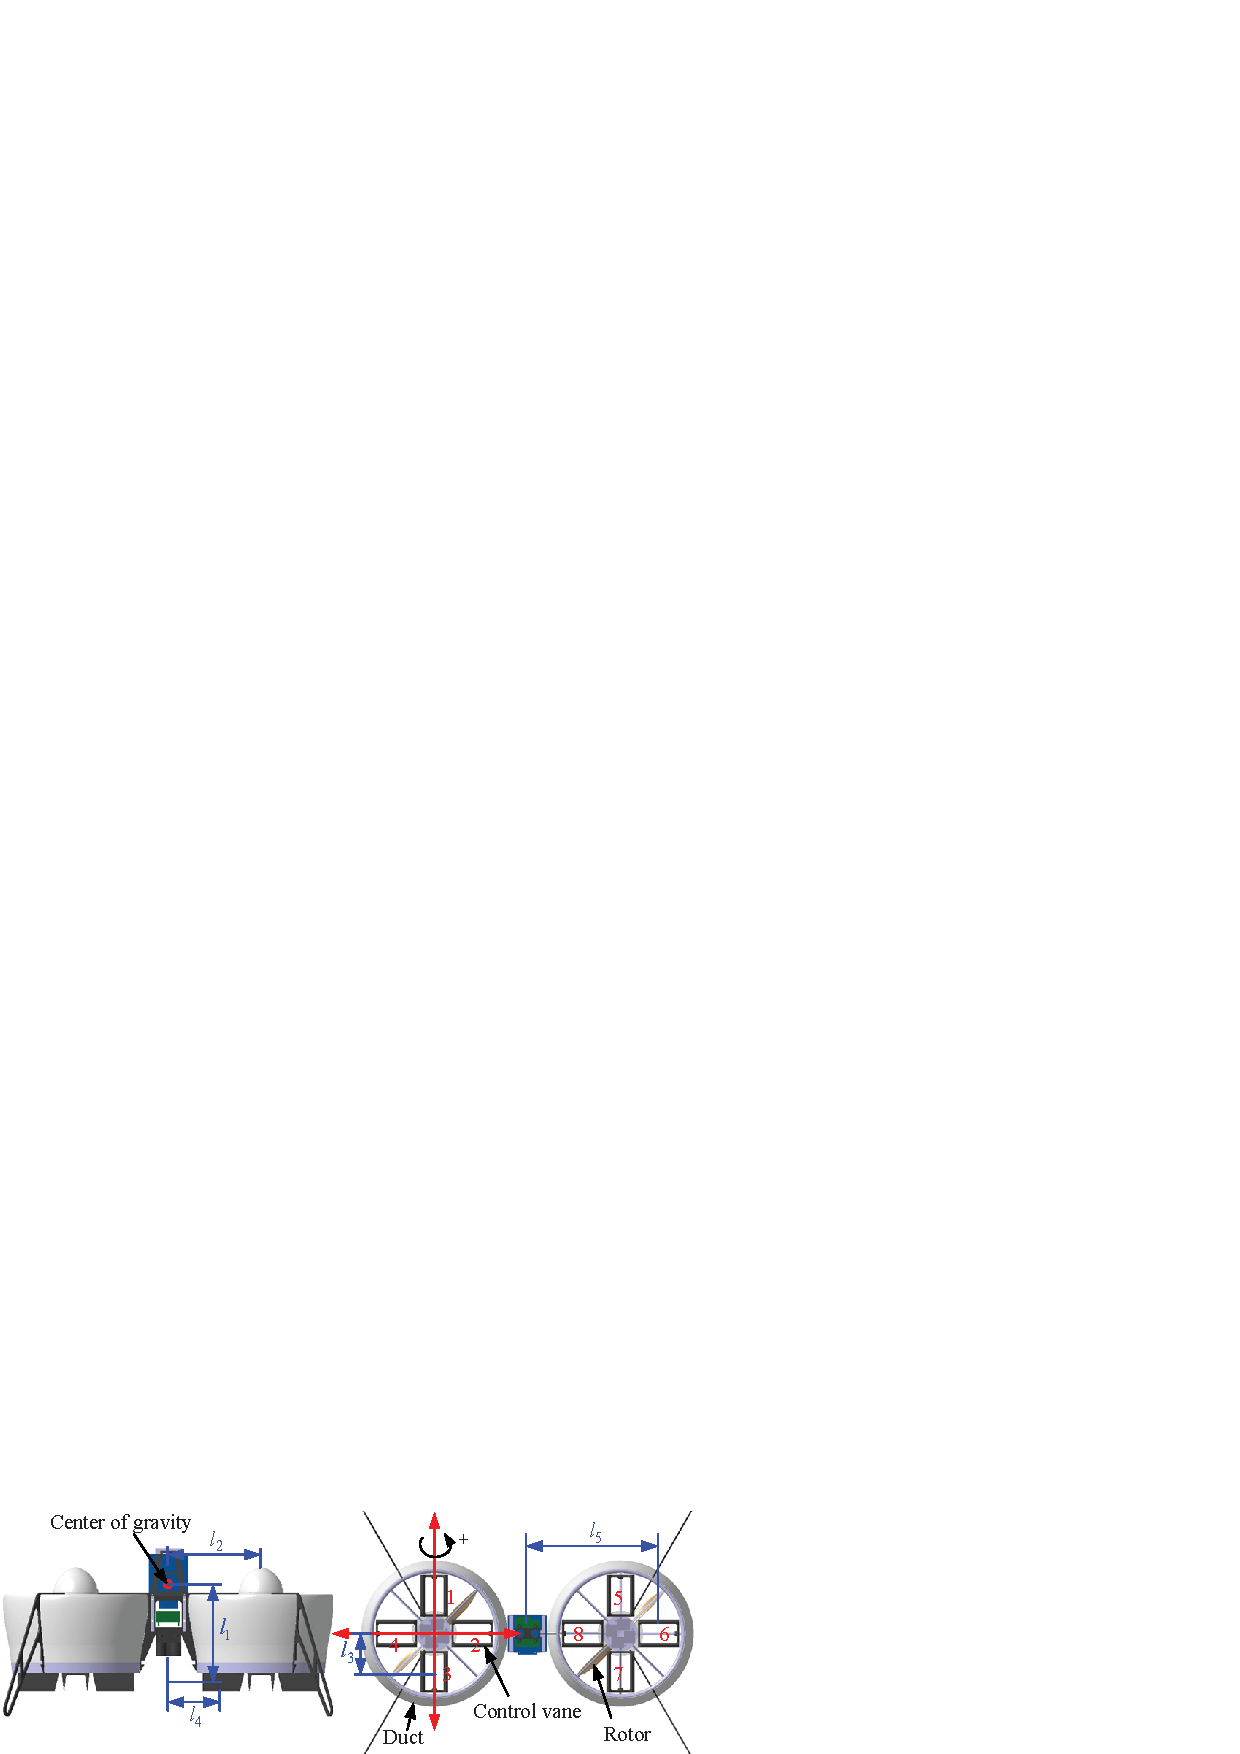
\includegraphics[scale=1]{Fig/Fig2.pdf}}
%		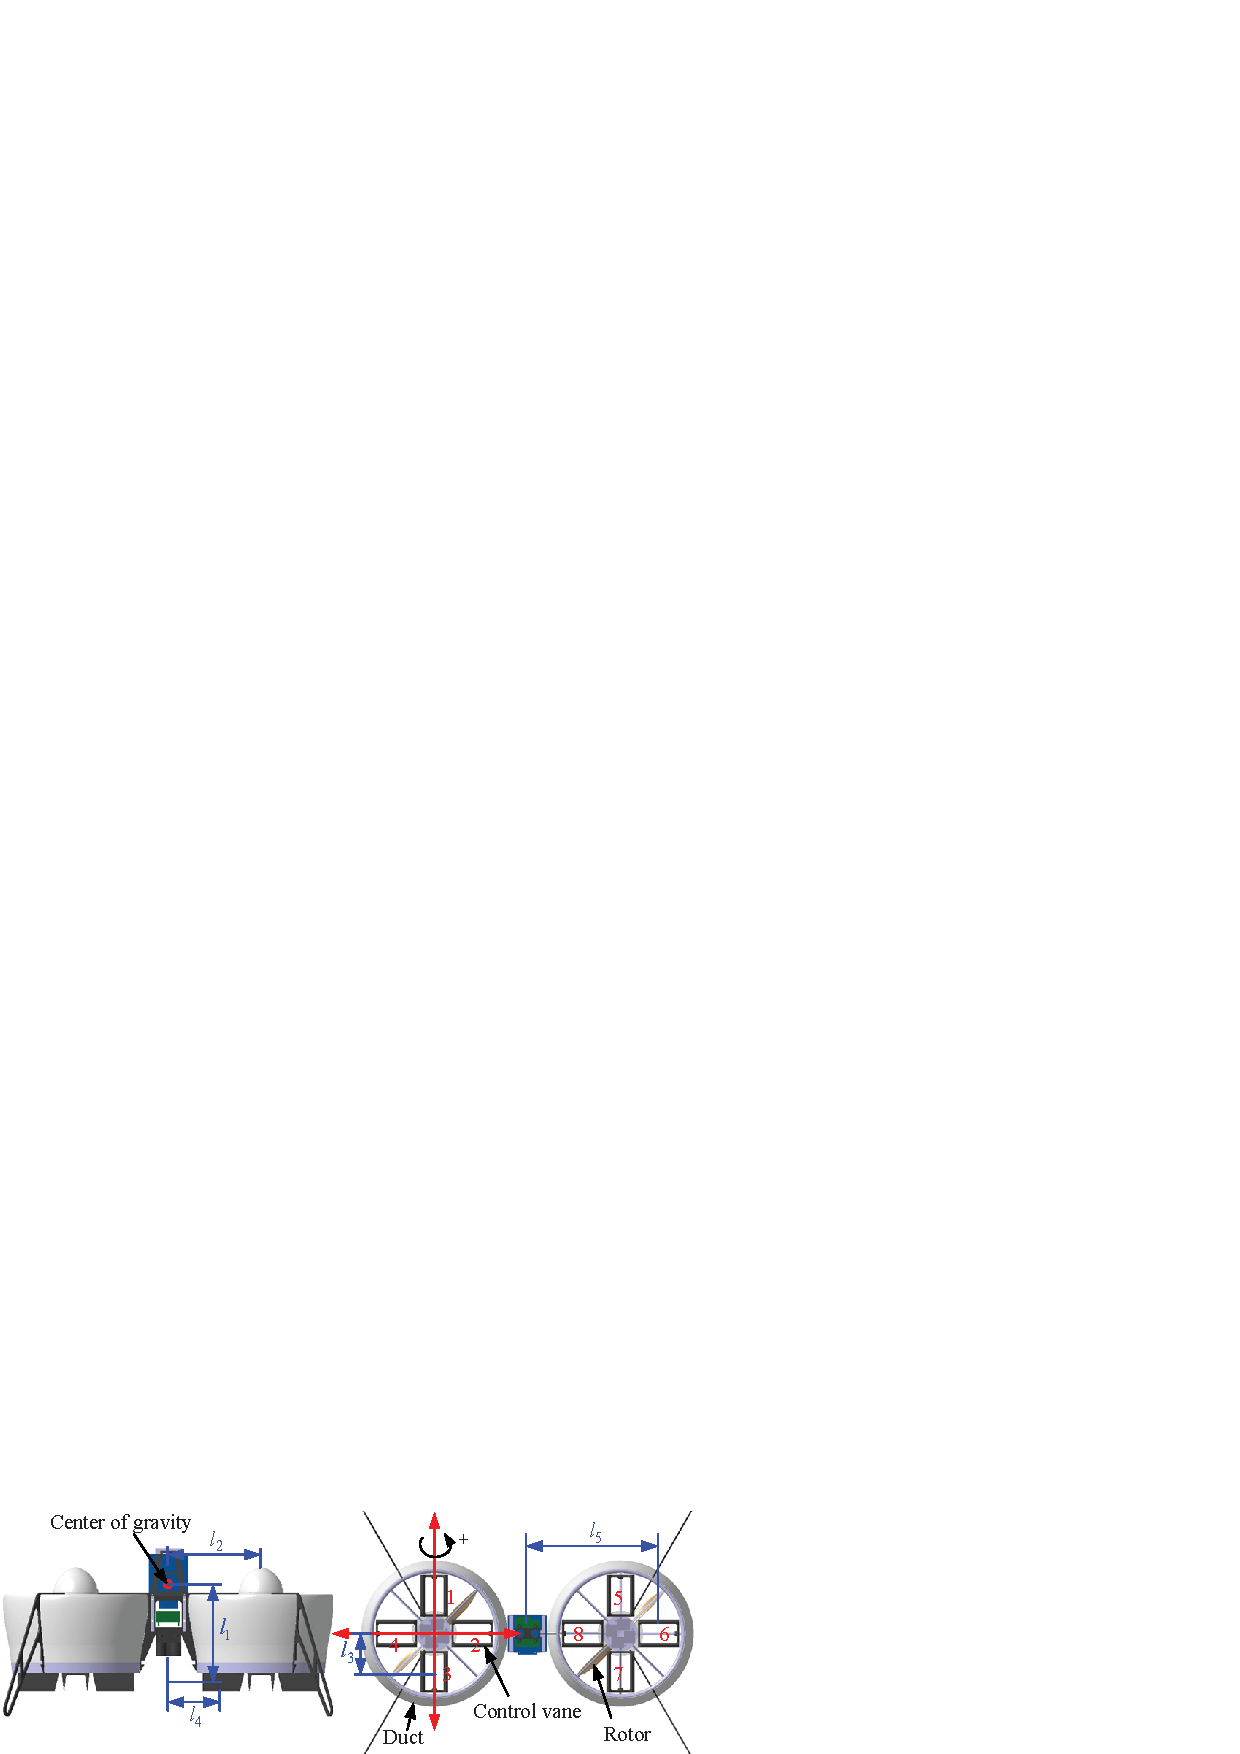
\includegraphics[scale=1]{Fig/Fig2.pdf}
%	\end{minipage}%
%	\begin{minipage}[c]{0.55\textwidth}
%		\centering
%%		\fbox{\includegraphics[scale=1.2]{Fig/Fig3.pdf}}
%		\includegraphics[scale=1.2]{Fig/Fig3.pdf}
%	\end{minipage}\\[1pt]
%	\begin{minipage}[t]{.45\textwidth}
%		\caption{\label{fig_euler}欧拉角及坐标系定义}
%	\end{minipage}%
%	\begin{minipage}[t]{.55\textwidth}
%		\caption{\label{arm}力臂示意图}
%	\end{minipage}%
%\end{figure}
定义操纵面旋转轴如图\ref{DFUAV_arm}所示,其中1号、2号操纵面旋转轴分别和机体系$ \bm{X}_b $轴和$ \bm{Y}_b $轴方向相同,1、3号操纵面产生滚转力矩,2、4号操纵面产生俯仰力矩。所有操纵面用于产生偏航力矩。规定操纵面旋转符合右手系则操纵面偏转角$\delta_i  $,$ i=1,2,3,4 $为正值,否则为负值。零偏转定义在操纵面平行于${{\bm{Z}}_{B}}$轴的位置。每个操纵面最大转动角度均为$\pm {{20}^{{}^\circ }}$。力臂${{l}_{1}}$、${{l}_{2}}$如图\ref{DFUAV_arm}所示。则每个操纵面上产生的升力可表示为\cite{Wu_2011,Zhao_2015,Graf_2008}
\begin{align}\begin{array}{l}
%F_{i}=\dfrac{1}{2} \rho S_{v} (V_i+V_c)^{2} C_{v} 
F_{i}=  k_{\delta} (V_i+V_c)^{2} \delta_{i} 
\end{array}	\label{F_i}
\end{align}
%\begin{align}\begin{array}{l}
%D_{\delta i}=  k_{D} F_{i}^{2}
%\end{array}\end{align}
其中$  k_{\delta} $为操纵面气动升力系数,和攻角$ \alpha_d $有关,$ V_i+V_c $为涵道出口气流流速。由操纵面产生的作用于机体的力和力矩可分别表示为\cite{Pflimlin_2007a}
\begin{align}
\bm{F}_{c}=\begin{bmatrix}
F_4-F_2	\\
F_1-F_3 \\
0
%D_{\delta 1}+D_{\delta 2}+D_{\delta 3}+D_{\delta 4}
\end{bmatrix}
\end{align}
\begin{align}\bm{M}_{c}=
\begin{bmatrix}
\tau_{x } \\
\tau_{y } \\
\tau_{z }
\end{bmatrix}
=
\begin{bmatrix}
-{{l}_{1}}\left(F_{1}-F_{3}\right) \\
{{l}_{1}}\left(F_{4}-F_{2}\right) \\
{{l}_{2}}\left(F_{1}+F_{2}+F_{3}+F_{4}\right)
\end{bmatrix}	\label{eq_M_c}
\end{align}
其中$ \bm{M}_{c} $又称驱动力矩,$ \tau_{x } $、$ \tau_{y } $、$ \tau_{z } $为驱动力矩在机体系坐标轴上的投影。在下一章控制系统设计中,控制律将给出期望的驱动力矩。
%\begin{align}
%%V_{e}=\frac{V_{0} \cos \alpha+\sqrt{\left(V_{0} \cos \alpha\right)^{2}+\frac{4 F_{t}}{\rho A_{d}}}}{2} \\
%C_{v}=C_{\delta}\left(\delta_{i}+\delta_{0}+\delta_{p}\right)
%\end{align}
%其中$ \rho $为流体密度,$ S_{v} $为操纵面面积,$ V_i+V_c $为涵道出口气流流速,$ C_{v} $为升力系数,$ C_{\delta} $为升力系数的斜率,$ \delta_{i} $、$ \delta_{0} $分别为操纵面偏转角和操纵面翼型的零升力偏转角度。当无人机向前飞行时,操纵面同时处于涵道风扇的尾流和前向飞行来流中。 合成气流方向和涵道的机体系$ z $轴成一个偏斜角$ \delta_{p} $,可表示为\cite{Tobias_2008a}
%\begin{align}\delta_{p}=\arctan \frac{\eta V_b \sin \alpha_d}{v_b+w \cos \alpha_d}\end{align}

%其中$\bm{\delta}$
% $k_{\delta}$为操纵面气动力系数, $V_d$为涵道底部吹出的气流速度。
%由于控制表面是可移动的平板提升表面,因此它们产生的提升力将取决于它们的有效攻角。 迎角是控制表面挠度,局部气流速度和由导管引起的向下冲洗的函数。 由于控制面的位置远离重心,因此包含了一些术语以说明由于车辆的角速度而引起的气流。 以下表达式指定这些影响如何影响升力,副翼和舵的迎角:
%\begin{align}\begin{array}{c}
%\alpha_{e}=\delta_{e}+\tan ^{-1}\left(-v_{x}-\omega_{y} l_{e}, v_{i}-v_{z}\right)-\gamma_{x} \\
%\alpha_{a}=-\delta_{a}+\tan ^{-1}\left(-v_{y}+\omega_{x} l_{a}, v_{i}-v_{z}\right)-\gamma_{y} \\
%\alpha_{r}=\delta_{r}+\tan ^{-1}\left(-\omega_{z} l_{r}, v_{i}-v_{z}\right)
%\end{array}\end{align}
%在这些表达式中,$ \delta $项表示控制面的挠度,而$ l $项表示控制面的空气动力学中心与车辆重心之间的距离。 术语“升降机”,“副翼”和“方向舵”在直升机模式下应用于控制面。 因此,舵表示风管流出的叶片,升降舵和副翼是位于机身末端的控制面。
%
%类似地,可以通过为每个控制面包括适当的速度分量来找到每个控制面所经历的动压力的表达式:
%\begin{align}\begin{array}{c}
%q_{e}=\dfrac{1}{2} \rho_{\infty}\left[\left(v_{i}-v_{z}\right)^{2}+\left(v_{x}+\omega_{y} l_{e}\right)^{2}\right] \\
%q_{a}=\dfrac{1}{2} \rho_{\infty}\left[\left(v_{i}-v_{z}\right)^{2}+\left(v_{y}-\omega_{x} l_{a}\right)^{2}\right] \\
%q_{r}=\dfrac{1}{2} \rho_{\infty}\left[\left(v_{i}-v_{z}\right)^{2}+\left(\omega_{z} l_{r}\right)^{2}\right]  \label{dynamic_pressure}
%\end{array}
%\end{align}
%
%使用式\eqref{dynamic_pressure}具有用于各种控制表面的适当参数,基于控制表面迎角提供了控制表面升力系数。这使我们能够找到与车身轴线垂直的提升力分量以及这些力产生的力矩。
%\begin{align}
%\begin{array}{c}
%\bm{F}_{\mathrm{cs}}=\left[\begin{array}{c}
%\operatorname{sgn}\left(v_{i}-v_{z}\right) C_{L, e} q_{e} \cos \left(\alpha_{e}-\delta_{e}\right) S_{e} \\
%\operatorname{sgn}\left(v_{i}-v_{z}\right) C_{L, a} q_{a} \cos \left(\alpha_{a}+\delta_{a}\right) S_{a} \\
%0
%\end{array}\right] \\
%\bm{M}_{\mathrm{cs}}=\left[\begin{array}{c}
%-\operatorname{sgn}\left(v_{i}-v_{z}\right) C_{L, a} q_{a} \cos \left(\alpha_{a}+\delta_{a}\right) S_{a} l_{a} \\
%\operatorname{sgn}\left(v_{i}-v_{z}\right) C_{L, e} q_{e} \cos \left(\alpha_{e}-\delta_{e}\right) S_{e} l_{e} \\
%\operatorname{sgn}\left(v_{i}-v_{z}\right) C_{L, r} q_{r} \cos \left(\alpha_{r}-\delta_{r}\right) S_{r} l_{r}
%\end{array}\right]
%\end{array}\end{align}
%S项代表每个控制表面的总面积。 请注意,对于操纵面,阻力和力矩的影响已被忽略。
\subsection{固定气动面动力学和陀螺力矩}
单涵道无人机内部设计固定气动面以平衡悬停状态下风扇反扭距的影响。如图\ref{F_af}所示,
%单个固定气动面上的力$ F_af $为:
%\begin{align}
%F_{a f}=\int d F \\
%d F=\frac{1}{2} \rho c_{a f} V_{a f}^{2} C_{L a f} \cdot d R
%\end{align}
%其中$ c_af $为单个气动面的弦长,$ R $为半径,$ V_{af} (R)=√((ω_w R)^2+(V_c+V_i )^2 ) $为入流速度,$ C_{Laf}=C_{laf} \alpha_{af} $为气动面的升力系数,$ C_{laf} $为翼型的升力线斜率,$ \alpha_{af} $为入流的有效迎角,满足:
%\begin{align}
%\alpha_{a f}=\varphi_{b}+\varphi_{0}
%\end{align}
%其中,$ φ_b $为旋转流场的入流角,
固定气动面对涵道轴的力矩可近似为:
\begin{align}\bm{M}_{a f}=\left(V_{c}+V_{i}\right)^{2} \varphi_{0}\left[\begin{array}{c}
0 \\
0 \\
d_{a f}
\end{array}\right]+\left(V_{c}+V_{i}\right) \varpi \left[\begin{array}{c}
0 \\
0 \\
d_{d s}
\end{array}\right]	\label{M_af}
\end{align}
其中$ d_{af} $ 、$ d_{ds} $为常系数,$ \varphi_0 $为气动面安装角。
\begin{figure}[htbp]
	\centering
	\includegraphics[scale=1]{Fig/F_af1.pdf}
	\caption{\label{F_af}固定气动面上的流场及气动力}
\end{figure}

在悬停点附近,涵道风扇转速几乎恒定,只有在剧烈的机动飞行中,转速变化才会比较明显。 为简单起见,假设风扇转速的变化可以忽略不计。 因此,由风扇的旋转产生陀螺力矩可表示为
\begin{align}
\bm{M}_{{g}}=-\bm{\omega} \times \bm{L}_{{r}}=b I_{b} \varpi
\begin{bmatrix}
-q \\
p \\
0
\end{bmatrix}
\end{align}
其中$ I_{b} $为风扇转动惯量,$ \bm{L}_{{r}} $为风扇角动量。
\section{双涵道动力学分析}
在悬停工作点附近,双涵道的动力学模型可以由单涵道推广而来,其左侧涵道和上述单涵道类似,右侧涵道是左侧的镜像,即风扇反向旋转且固定气动面反向安装。在双涵道中,总的气动力$ \bm{F} $是左右两个涵道所受气动力的矢量和,记为
\begin{align}
\bm{F}&=\bm{F}_{L}+\bm{F}_{R}
\end{align}
其中$ \bm{F}_{L} $为左边涵道所受气动力,$ \bm{F}_{R} $为右边涵道所受气动力。其表达式和单涵道类似,以$ \bm{F}_{L} $为例,可以表示为
\begin{align}
\bm{F}_{L} &=\bm{F}_{La}+\bm{F}_{Lr}+\bm{F}_{Ld}+\bm{F}_{Lc} 
\end{align}
$ \bm{F}_{R} $的表达式完全类似。类似的,总的气动力矩力矩$ \bm{M} $可表示为
\begin{align}
\bm{M}&=\bm{M}_{L}+\bm{M}_{R}
\end{align}
其中$ \bm{M}_{L} $为左边涵道所受气动力矩,$ \bm{M}_{R} $为右边涵道所受气动力矩。以左侧涵道为例,由力和力矩的关系,气动力矩可表示为
\begin{align}
\bm{M}_{L} &=\bm{l} \times \bm{F}_{L}  
\end{align}
其中矢量$ \bm{l} $力的作用点在机体系的坐标表示。本节仅讨论和本文主题相关双涵道操纵面动力学部分,详细的双涵道建模可参考\cite{Speck_2013,Speck_2013a}。
%\subsection{机身动力学}
%机身空气阻力产生的力可以写为:
%\begin{align}
%\bm{F}_{{a}} = \bm{F}_{{La}}+\bm{F}_{{Ra}}
%\end{align}
%其中$ \bm{F}_{{La}} $、$ \bm{F}_{{Ra}} $的表达式由式\eqref{eq_F_a}确定。对应的力矩为
%\begin{align}
%\bm{M}_{{a}} = \bm{M}_{{La}}+\bm{F}_{{Ma}}= \bm{l}_{aL} \times \bm{F}_{{La}}+ \bm{l}_{Ra} \times \bm{F}_{{Ra}}
%\end{align}
%其中$ \bm{l}_{aL} $、$ \bm{l}_{aR} $分别代表左、右侧涵道的机身气动力作用点在机体系的坐标表示。。
\subsection{涵道风扇动力学}
作用于无人机的推力
\begin{align}
\bm{F}_{r}=\bm{F}_{{Lr}}+\bm{F}_{{Rr}}=\begin{bmatrix}
0\\0\\
-T_{La}-T_{Ra}
\end{bmatrix}
\end{align}
其中$ T_{{La}} $、$ T_{{Ra}} $的表达式由上一节求解$ T_a $的方法确定。考虑到风扇上的升力差会产生一个滚转力矩,因此风扇产生的扭矩可表示为
\begin{align}
\bm{M}_{r}=\begin{bmatrix}
(T_{La}-T_{Ra})l_2\\0\\
Q_{L}-Q_{R}
\end{bmatrix}	\label{eq_prop}
\end{align}
其中$ Q_{R} $前的负号是由于右边的风扇是顺时针转动的,$ l_2 $为两个涵道风扇的旋转中心的距离,$ Q_{L}$、$Q_{R} $类似的由式\eqref{eq_Q}确定。
%\subsection{涵道动力学}
%左右两侧的动量阻力完全类似,总的动量阻力表示为
%\begin{align}
%\bm{F}_{m}=\bm{F}_{{Lm}}+\bm{F}_{{Rm}}
%\end{align}
%测风产生的力矩为
%\begin{align}
%\bm{M}_{{l}}=\bm{l}_{Lm} \times \bm{F}_{{Lm}}+\bm{l}_{Rm} \times \bm{F}_{{Rm}}
%\end{align}
%其中$ \bm{l}_{Lm} $、$ \bm{l}_{Rm} $为力臂矢量。
%
%参照上一节,涵道产生的力和力矩可分别表示为
%\begin{align}
%\bm{F}_{{d}}=
%\begin{bmatrix}
%L_{Lx}+L_{Rx}+D_{Lx}+D_{Rx} \\
%L_{Ly}+L_{Ry}+D_{Ly}+D_{Ry} \\
%L_{Lz}+L_{Rz}+D_{Lz}+D_{Rz}
%\end{bmatrix}
%+\bm{F}_{{m}} 
%\end{align}
%\begin{align}
%\bm{M}_{{d}}=
%\begin{bmatrix}
%(L_{Lx}+L_{Rx}) l_{d} \\
%(L_{Ly}+L_{Ry}) l_{d} \\
%0
%\end{bmatrix}
%+\bm{M}_{{l}}
%\end{align} 
\subsection{操纵面动力学}
类似单涵道,定义操纵面旋转轴如图\ref{TDFUAV_arm}所示,其中1号、2号操纵面旋转轴分别和机体系$ \bm{X}_b $轴和$ \bm{Y}_b $轴方向相同,1、3、5和7号操纵面产生滚转力矩,2、4、6和8号操纵面产生俯仰力矩。所有操纵面用于产生偏航力矩。零偏转定义在操纵面平行于${{\bm{Z}}_{B}}$轴的位置。操纵面偏转角$\delta_i  $,$ i=1,2,\ldots,8 $最大转动角度均为$\pm {{20}^{{}^\circ }}$。力臂如图\ref{DFUAV_arm}所示。每个操纵面上的升力$ F_i $由式\eqref{F_i}给出,为简单起见,忽略操纵面阻力,则操纵面气动力和驱动力矩可表示为
\begin{figure}[htbp]
	\centering	
	\includegraphics[scale=1]{Fig/TDFUAV_arm.pdf}%
	\caption{\label{TDFUAV_arm}双涵道力臂示意图}
\end{figure}
\begin{align}
\bm{F}_{c}=\begin{bmatrix}
-F_2+F_4-F_6+F_8	\\
F_1-F_3+F_5-F_7 \\
0
%D_{\delta 1}+D_{\delta 2}+D_{\delta 3}+D_{\delta 4}
\end{bmatrix}
\end{align}
\begin{align}\bm{M}_{c}=
\begin{bmatrix}
\tau_{x } \\
\tau_{y } \\
\tau_{z }
\end{bmatrix}
=
\begin{bmatrix}
-{{l}_{1}}\left(F_1-F_3+F_5-F_7\right) \\
{{l}_{1}}\left(-F_2+F_4-F_6+F_8\right) \\
\left(l_3 F_{1} - l_4 F_{2} + l_3 F_{3} + l_5 F_{4} + l_3 F_5 + l_5 F_6 + l_3 F_7 + -l_4 F_8 \right)
\end{bmatrix}	\label{eq_TDF_M_c}
\end{align}	
%\subsection{固定气动面动力学和陀螺力矩}
%双涵道内部的固定气动面完全类似单涵道,并且左右两边互为镜像,即旋翼(风扇)转动方向相反,固定气动面安装方向相反。双涵道固定气动面对涵道轴的力矩可表示为:
%\begin{align}
%\bm{M}_{a f}=\bm{M}_{Laf}+\bm{M}_{Raf}
%\end{align}
%其中$ \bm{M}_{Laf} $ 、$\bm{M}_{Raf} $分别与左右两侧涵道的旋翼转速相关,由式\eqref{M_af}确定。旋翼的旋转产生陀螺力矩表示为
%\begin{align}
%\bm{M}_{{g}}=-\bm{\omega} \times (\bm{L}_{{Lr}}-\bm{L}_{{Rr}})=b (I_{Lb}\varpi_L-I_{Rb}\varpi_R)
%\begin{bmatrix}
%-q \\
%p \\
%0
%\end{bmatrix}
%\end{align}
%其中$ I_{Lb} $、$ I_{Rb} $为左右两侧旋翼转动惯量,$ \varpi_L $、$ \varpi_R $为左右两侧旋翼转速。
\section{涵道无人机仿真模型}
利用CDF计算得涵道模型参数如表\ref{DF_para}、表\ref{TDF_para}所示,其中表\ref{TDF_para}仅列出和单涵道不同的参数。将上述与力和力矩有关的方程用借助MATLAB$^\circledR$/Simulink$^\circledR$的S-函数实现,式\eqref{eq_nonlinear_model}用Simulink$^\circledR$库自带的六自由度刚体模块实现,被控对象的仿真图如图\ref{fig_plant_simulink}所示。其中“Actuators”表示操纵面偏转角$ \bm{\delta} $信号输入,“Environment”表示状态反馈和环境变量(重力,风扰等)。“Calculate Force”表示计算作用于无人机的力,“Calculate Torque”表示计算作用于无人机的力矩,这两个模块内部分别如图\ref{fig_force_simulink}、图\ref{fig_moment_simulink}所示,其中$\mathrm{R}^{\wedge} \mathrm{T}$ 表示$ R^T $,“$ \mathrm{s\_{}Force} $”是计算作用于无人机的气动力的S-函数,“$ \mathrm{s\_{}Torque} $”是计算作用于无人机的气动力矩的S-函数。

\begin{table}
\caption{\label{DF_para}单涵道模型参数}
	\centering{}%
	\small 
	\begin{tabular}{cccccc}
		\hline 
		参数符号 & 数值&参数符号 & 数值&参数符号 & 数值\tabularnewline
		\hline 
		$ A_x,A_y,A_z $  & $ 0.04082\,\text{m}^2 $ &$ \rho $        &$1.225\,\text{kg}/\text{m}^3$&$ I_b $           & $ 0.000029 $               \tabularnewline
		$ k_{\varpi} $   & $1.13342 \times 10^{-6}$& $ d_{\varpi} $ & $1.13342 \times 10^{-7}$ 	  &$k_{\delta} $     & $ 0.01495 $ 			      \tabularnewline
		$C_{D,x},C_{D,y}$& $ 0.43213 $             &$ C_{D,z} $     & $ 0.13421 $             	  &	$ q_a $ 	     & $ 1.49 $ 				  \tabularnewline
	    $ l_{a} $        & $ -0.1121\,\text{m} $   & $ d_{ds} $     & $ 0.01495 $			  	  &$ d_{af} $        & $ 0.01495 $    			  \tabularnewline
		$ R $            & $ 0.11\,\text{m} $      &$ b $           & $ 2 $       			   	  &$ S $ 			 & $ 0.04082\,\text{m}^2 $    \tabularnewline
		$C_{l_{\alpha}}$ & $ 2.212\,/\text{rad} $  &$C_{l, \max } $ & $ 1.05 $ 				   	  &$ C_{l, \min } $  & $ -1.05 $ 				  \tabularnewline
		$ l_2 $          & $ 0.06647\,\text{m} $   &$ l_1 $         & $ 0.17078\,\text{m} $    	  &	$ m $ 		     & $ 1.53\,\text{kg} $ 		  \tabularnewline
		$ C_{d, o } $    & $ 0.9 $                 &$ C_{d, g } $   & $ 0.9 $					  &$ C_{duct} $      & $ 0.78497 $	 			  \tabularnewline
		$ I_x $          & $ 0.02548 $ 			   &$ I_y $         & $ 0.02550 $                 &$ I_z $			 & $ 0.00562 $ 				  \tabularnewline
		\hline 
	\end{tabular}	
\end{table}

\begin{table}
	\caption{\label{TDF_para}双涵道模型参数}
	\centering{}%
	\small 
%	\resizebox{\textwidth}{!}{
	\begin{tabular}{cccccc}
		\hline 
		参数符号 & 数值&参数符号 & 数值&参数符号 & 数值\tabularnewline
		\hline 
		$ I_x $ & $ 054593 $ &$ I_y $ & $ 0.017045 $& $ I_z$ & $ 0.049226 $ \tabularnewline
	    $ l_{1} $ & $ 0.0808\,\text{m} $&$ l_{2} $ & $ 0.175\,\text{m} $ &$ l_3 $ & $ 0.06647\,\text{m} $ \tabularnewline 
		$ l_4 $ & $ 0.2415\,\text{m} $ &$ l_5 $ & $ 0.1085\,\text{m} $& $ m $ & $ 3.7\,\text{kg} $ \tabularnewline
		\hline 
	\end{tabular}	%}
\end{table}
\begin{figure}[htbp]
	\centering
	\includegraphics[scale=0.35]{Fig/Fig_model.png}
	\caption{\label{fig_plant_simulink}被控对象simulink}
\end{figure}
\begin{figure}[htbp]
	\centering
	\includegraphics[scale=0.3]{Fig/Fig_Force.png}
	\caption{\label{fig_force_simulink}Calculate Force模块}
\end{figure}
\begin{figure}[htbp]
	\centering
	\includegraphics[scale=0.32]{Fig/Fig_Torque.png}
	\caption{\label{fig_moment_simulink}Calculate Torque模块}
\end{figure}
\section{本章小结}
本章建立了涵道风扇式无人机的数学模型。首先对无人机的运动进行参数化,定义了坐标系。然后推导了运动方程,再对运动方程中涉及的气动力和气动力矩进行分析。最后根据所建立的模型建立MATLAB$^\circledR$/Simulink$^\circledR$仿真,仿真中将该模块作为被控对象,然后针对该对象设计控制器以及分配器。





%\subsection{旋翼模型}
%旋翼模型基于基本动量理论和叶片元素理论进行推导的,这里的推导类似直升机的旋翼模型的推导,虽然并不能解决管道中的不稳定气流的建模问题,但有证据表明这种模型确实提供了对旋翼性能的足够准确的刻画\cite{Johnson_2005}。经过旋翼的气流流速受沿机体$ z $轴的速度$ w$以及旋翼叶片的转速和旋翼叶片的几何形状影响,可表示为\cite{Heffley_1988}
%\begin{align}
%V_i+V_c=w+\dfrac{2}{3} \varpi r\left(\dfrac{3}{4} K_{t w i s t}\right)
%\end{align}
%其中$ \varpi $代表旋翼转速,$ r $是旋翼半径,而$ K_{t w i s t} $是叶片的扭转。 推力现在可以写成\cite{Heffley_1988}
%\begin{align}
%F_T=\dfrac{1}{4}\left(V_i+V_c-v_{i}\right) \varpi r^{2} \rho_{\infty} a_{0} b c_{r}
%\end{align}
%其中,$ v_{i} $表示通过旋翼处气流的的诱导速度,$ a_{0} $表示旋翼升力曲线斜率,$ b $表示旋翼的叶片数,$ c_{r} $是旋翼叶片的弦长。 涵道远端的气流速度可以表示为\cite{Stepniewski_2013}
%\begin{align}
%v^{\prime}=\sqrt{u^{2}+v^{2}+\left(w-v_{i}\right)^{2}}
%\end{align}
%现在可以将诱导速度表示为\cite{Stepniewski_2013}
%\begin{align}
%v_{i}=\dfrac{F_T}{2 \rho_{\infty} \pi r^{2} v^{\prime}}
%\end{align}
%这些方程是迭代求解的。 综上,作用在无人机上的旋翼产生的推力可以表示为
%\begin{align}
%\bm{F}_{r}=\begin{bmatrix}
%0\\0\\
%-F_T
%\end{bmatrix}
%\end{align}
%
%施加在旋翼上的反扭矩表达式需要功率来计算。 诱导功率和翼型功率为\cite{Heffley_1988}
%\begin{gather}
%P_{i}=\tau\left(v_{i}-w\right) \\
%P_{p}=\dfrac{1}{8} \rho_{\infty} f_{r} r \varpi\left[\left(r \varpi\right)^{2}+4.6\left(u^{2}+v^{2}\right)\right]
%\end{gather}
%$ f_{r} $代表旋翼摩擦项,有\cite{Heffley_1988}
%\begin{align}
%f_{r}=C_{D_{o}} r b c_{r_{r}}
%\end{align}
%空气施加在旋翼上的力矩可以表示为\cite{Johnson_2005}
%\begin{align}M_{r}=\dfrac{P_{i}+P_{p}}{\omega_{r}}\end{align}
%发动机功率与旋翼转速和油门位置的关系可表示为\cite{Johnson_2005}
%\begin{align}
%P_{e}=\dfrac{x_{thr} K_{b} \eta_{e} \min \left(\varpi K_{d}, K_{r }\right)}{K_{r }}
%\end{align}
%其中$ x_{t}  $表示油门位置,$ K_{b} $是发动机的马力,$ \eta_{e} $是发动机效率,$ K_{d} $是主风扇齿轮比,而$ K_{r} $是发动机每秒的最大转数。 控制油门状态的微分方程为
%\begin{align}
%\dot{x}_{t}=\dfrac{\delta_{t}-x_{t}}{K_{t}}
%\end{align}
%其中$ \delta_{t} $表示油门输入,$ K_{t} $是发动机时间常数。 从顶部看时旋翼是逆时针旋转的,发动机施加的力矩可表示为
%\begin{align}
%M_{e}=\dfrac{P_{e}}{\varpi K_{d}} 
%\end{align}
%\begin{gather}
%\bm{M}_{{r}}=\begin{bmatrix}
%0 \\
%0 \\
%M_{e} K_{d}
%\end{bmatrix}	\label{M_rotor}
%\end{gather}
%最后,控制风扇转速的微分方程为
%\begin{align}
%\dot{\bar{\omega}}_{r}=\dfrac{M_{e} K_{d}-M_{r}}{b i_{b}}
%\end{align}
%其中$ i_{b} $表示单个叶片绕旋转轴的惯性矩。













	%\chapter{涵道风扇式无人机的控制分配问题}
\chapter{涵道风扇式无人机的自抗扰控制}
%
通过上一章的建模分析,从涵道飞行器的动力学模型可以看出,涵道无人机在飞行过程中受到复杂气动力和气动力矩的影响。对于姿态控制而言,不仅受舵面的驱动力矩作用,还受固定气动面的平衡扭矩、风扇扭矩、陀螺力矩、气动俯仰力矩的作用。这些力矩难以得到其解析形式,但却极大的影响飞机飞行性能。比如,飞机在进行高度控制的过程中需要改变螺旋桨转速,但这同时将因为转速的改变而直接改变系统受到的陀螺力矩、平衡扭矩、风扇扭矩。在存在外扰动时,如果不合理的转换控制力矩到各个舵面偏转角,那么舵面提供的驱动力矩很可能不能抵消这些扰动,从而使系统发散。要使姿态控制更为稳健,首先需要估计这些扰动,对扰动进行补偿之后将控制量转换成舵面偏转角。本节将介绍一种扰动抑制控制算法,将其改进后应用到涵道无人机的姿态控制中。
\section{从PID控制到自抗扰控制}
PID控制器根据系统输入和参考输入的误差进行控制,用误差来消除误差,而不需要知道系统的数学模型。因其参数调节过程简单,参数物理意义明确,在工程实践中得到广泛应用。然而随着科技的发展,工业界对控制器性能的要求越来越高,PID控制的缺点日益明显,主要有:
\begin{enumerate}
	\item PID控制律是基于参考信号与系统输出的误差进行计算的。物理系统的输出通常光滑的,但输入参考信号往往是不光滑的阶跃信号。这一矛盾导致误差的初始值往往比较大,进而使得系统受到较大的冲击产生超调和震荡。为了减小超调,通常是减小控制器增益,但又会使得调节时间变长。即PID控制器存在快速性和超调之间的矛盾。
	\item 实际系统中噪声的存在使得微分器难以实现。
	\item PID控制律是误差的比例、积分、微分的线性组合,组合方式并非最优。
	\item 积分器虽然可以消除静态误差,但会产生积分饱和导致大超调和震荡次数的增加,使系统不稳定。 
\end{enumerate}

针对PID控制的不足,ADRC做了如下改进:
\begin{enumerate}
	\item 为参考输入安排过渡过程:根据系统的阶次安排合适的过渡过程,解决超调和快速性之间的矛盾。使得误差反馈增益的取值范围更大,同时给定的反馈增益能适用于更多的系统,控制器鲁棒性增强。
	\item 提取微分信号:设计非线性微分跟踪器来提取参考输入的微分,降低噪声的影响。同时还设计扩张状态观测器提取反馈信号的微分。
	\item 非线性误差反馈:对误差的比例、微分应用非线性组合构建控制量,得到比线性组合更好的效果。
	\item 估计总和扰动:应用ESO实时估计系统的总和扰动,在控制律中包含扰动补偿,避免了积分反馈的副作用,同时提高了系统抗干扰能力。
\end{enumerate}
\section{自抗扰控制器原理}
自抗扰控制器由跟踪微分器(TD)、扩张状态观测器(ESO)以及非线性误差反馈(NLESF)组成。自抗扰控制技术不依赖于对象的数学模型,通过扩张状态观测器实时估计出包含系统内部模型不确定性和外部扰动不确定性的总扰动,通过动态补偿的方法,将实际系统补偿为积分串联型的标准结构。ADRC的收敛性最初由文献\parencite{HanJingQing_2008}给出分析。近年来,郭宝珠等人给出了更严格的数学证明,在文献\parencite{Guo_2010,Guo_2011b,Guo_2011c,Guo_2011d}给出了跟踪微分器的收敛性证明。文献\parencite{Guo_2011,Guo_2011a,Guo_2012,Zhao_2016}给出了扩张状态观测器的收敛性证明,文献\parencite{Guo_2013,Zhao_2016a,Guo_2013,Guo_2012a}分析了ADRC闭环系统的收敛性。本节将逐一介绍其原理,并不加证明地给出几条收敛性定理。
\subsection{跟踪微分器}
物理系统通常有一定的惯性,其状态一般不会突变,而参考输入却可能会是突变信号。因此在跟踪问题中,要求系统跟随突变信号是不合理的。利用跟踪微分器产生参考指令的过渡过程和提取微分信号,使得系统初始误差更为合理。借助微分跟踪器,系统可以使用更大的控制增益,可提高系统快速性。

可设计如下形式的二阶跟踪微分器
\begin{align}
\left\{\begin{array}{l}
\dot{v}_{1}(t)=v_{2}(t) \\
\dot{v}_{2}(t)=R^{2}\left(-\zeta_{1}\left[v_{1}(t)-v_c(t)\right]^{\alpha}-\zeta_{2}\left[\dfrac{v_{2}(t)}{R}\right]^{\beta}\right)
\end{array}\right.	\label{eq_sec_TD}
\end{align}
其中$ [r]^{\alpha}=\operatorname{sign}(r)\left|r\right|^{\alpha} $,且
\begin{align}
\zeta_{1}, \zeta_{2}>0, \alpha=\dfrac{b-1}{a}, \beta=\dfrac{b-1}{b}, a=b+1, b>1	\label{eq_para_sec_TD}
\end{align}
若选取适当参数,则TD的状态$ {v}_{1}(t) $即为所安排的过渡过程,$ v_{2}(t) $为参考输入$ v_c(t) $的微分信号。其收敛性可由如下定理给出\cite{Guo_2011b}:
\begin{theorem}
	如果待处理信号满足$ \sup\limits_{t \in[0, \infty ) }\left|v^{(i)}_c(t)\right|<\infty, i=1,2.$则跟踪微分器\eqref{eq_sec_TD}是收敛的,即对于任意的初始值和$\forall T_1 >0 $, $\exists R_0 >0 $使得对$\forall R>R_0 $及$ t>T_1 $,有
	\begin{align}
	\left|v_{1}(t)-v_c(t)\right| \leq M_{1}\left(\dfrac{1}{R}\right)^{\beta {\frac{1-\gamma}{\gamma}}}, \quad\left|v_{2}(t)-\dot{v}_c(t)\right| \leq M_{2}\left(\dfrac{1}{R}\right)^{\beta \frac{1-\gamma}{\gamma}-1}
	\end{align}
	其中$\gamma=\frac{l-1}{l}, l>\max \{1, a, b\}$,$ M_1 $、$M_2$是依赖于初始值的常数,$ \alpha $、$\beta$是满足式\eqref{eq_para_sec_TD}的参数。		\label{the_sec_TD}
\end{theorem}
\subsection{扩张状态观测器}
自抗扰控制的核心是设计扩张状态观测器,对系统未建模动态和外部扰动进行估计。通过在系统中实时补偿该“总和扰动”,使对象模型变成“积分器串联型”线性系统。考虑更具一般性的$ n $阶的情况,针对如下系统
\begin{align}\left\{\begin{array}{l}
x^{(n)}(t)=f\left(t, x(t), \dot{x}(t), \ldots, x^{(n-1)}(t)\right)+w(t)+bu(t) \\
y(t)=x(t)
\end{array}\right.	\label{eq_sys}
\end{align}
其中$ w(t) $为系统的外部扰动,简记为$ w $,$ f\left(t, x_{1}(t), x_{2}(t), \ldots, x_{n}(t)\right) $为系统内部不确定函数,简记为$ f $。将上式改写为
\begin{align}\left\{\begin{array}{l}
\dot{x}_{1}(t)=x_{2}(t),\quad
\dot{x}_{2}(t)=x_{3}(t)  \\
\vdots \\
\dot{x}_{n}(t)=f\left(t, x_{1}(t), x_{2}(t), \ldots, x_{n}(t)\right) +w(t)+bu(t)	\\
y(t)=x_{1}(t)
\end{array}\right.	\label{eq_n_diff}
\end{align}
并将$ f+w $扩充为新的状态,可设计扩张状态观测器\cite{Guo_2012}
\begin{align}\left\{\begin{array}{l}
\dot{\hat{x}}_{1}(t)=\hat{x}_{2}(t)+\varepsilon^{n-1} g_{1}\left(\dfrac{y(t)-\hat{x}_{1}(t)}{\varepsilon^{n}}\right)\\[3mm]
\dot{\hat{x}}_{2}(t)=\hat{x}_{3}(t)+\varepsilon^{n-2} g_{2}\left(\dfrac{y(t)-\hat{x}_{1}(t)}{\varepsilon^{n}}\right) \\
\vdots \\
\dot{\hat{x}}_{n}(t)=\hat{x}_{n+1}(t)+g_{n}\left(\dfrac{y(t)-\hat{x}_{1}(t)}{\varepsilon^{n}}\right)+bu(t) \\[3mm]
\dot{\hat{x}}_{n+1}(t)=\dfrac{1}{\varepsilon} g_{n+1}\left(\dfrac{y-\hat{x}_{1}(t)}{\varepsilon^{n}}\right)
\end{array}\right.  	\label{eq_NLESO}
\end{align}
使观测器状态$ \hat{x}_i,i=1,2,\dots,n+1 $分别收敛于系统状态$ x_1,x_2,\dots,x_n $以及$ f+w $。该观测器的收敛性结论需要如下几个假设\cite{Guo_2012,Guo_2011}:
\begin{assumption}
	函数$ f $,$ w $对所有自变量都是连续可微的,且满足
	\begin{align}|u|+|f|+|\dot{w}|+\left|\dfrac{\partial f}{\partial t}\right|+\left|\dfrac{\partial f}{\partial x_{i}}\right| \leq c_{0}+\sum_{j=1}^{n} c_{j}\left|x_{j}\right|^{k}\end{align}
	其中$c_{j}, j=0,1, \cdots, n$是正实数, $ k $是正整数。	\label{H1}
\end{assumption}	
\begin{assumption}
	外部扰动$w$和式\eqref{eq_n_diff}所示系统的解满足
	\begin{align}
	|w|+\left|x_{i}(t)\right| \leq \bm{B}
	\end{align}
	其中$ B>0 $,$ i=1,2,\cdots,n $,$ t>0 $。	\label{H2}
\end{assumption}
\begin{assumption}
	存在常数$ \lambda_i,i=1,2,3,4 $、$ \alpha $、$ \beta $以及连续的正定函数$ V,W:\mathbb{R}^{n+1} \rightarrow \mathbb{R} $满足下面三个条件
	\begin{enumerate}
		\item $ \lambda_{1}\|\bm{y}\|^{2} \leq V(\bm{y}) \leq \lambda_{2}\|\bm{y}\|^{2}, \quad \lambda_{3}\|\bm{y}\|^{2} \leq W(\bm{y}) \leq \lambda_{4}\|\bm{y}\|^{2} $ 
		\item $ \sum_{i=1}^{n} \frac{\partial V}{\partial y_{i}}\left(y_{i+1}-g_{i}\left(y_{1}\right)\right)-\frac{\partial V}{\partial y_{n+1}} g_{n+1}\left(y_{1}\right) \leq-W(\bm{y}) $ 
		\item $ \left|\frac{\partial V}{\partial y_{n+1}}\right| \leq \beta\|\bm{y}\| $		
	\end{enumerate}
	其中$\bm{y}=[y_{1} \quad y_{2} \quad \ldots \quad y_{n+1}]^{\top}$,$\|\cdot\|$表示$ \mathbb{R}^{n+1} $中的欧几里得范数	\label{H3}
\end{assumption}
\begin{theorem}
	若假设\ref{H1}、\ref{H2}以及\ref{H3}成立,那么有
	\begin{enumerate}
		\item 对于任意给定的$ a>0 $,$ \lim\limits_{\varepsilon \rightarrow 0}\left|x_{i}(t)-\hat{x}_{i}(t)\right|=0 $在$t \in [a, \infty)$上—致地成立	
		\item $ \lim\limits_{t \rightarrow \infty}\left|x_{i}(t)-\hat{x}_{i}(t)\right| \leq O\left(\varepsilon^{n+2-i}\right)  $
	\end{enumerate}
	其中$x_{i}$,$ \hat{x}_{i}$分别为式\eqref{eq_n_diff}所示系统和式\eqref{eq_NLESO}所示ESO的解,$i=1,2, \ldots, n+1$,$ x_{n+1}=f+w$是式\eqref{eq_n_diff}所示系统的扩张状态	\label{the_NLESO}
\end{theorem}
\subsection{非线性误差反馈}
在ADRC控制技术中,延拓了“基于误差来消除误差”的思想。将跟踪微分器得到的跟踪信号以及微分信号与ESO中得到的系统状态的估计信号做差,通过特定的组合产生误差反馈。与PID不同的地方在于,最终的控制量是在误差反馈的基础上添加一个扰动补偿项,将非线性系统线性化。误差反馈使线性化后的系统跟踪给定输入。

以$ n=2 $即二阶系统为例,由上文可知参考输入$ v_c $经过跟踪微分器得到的过渡过程及其微分信号为$ v_1 $、$ v_2 $,ESO估计的系统状态为$ \hat{x}_1 $和$ \hat{x}_2 $,由此定义状态误差
\begin{align}\begin{array}{l}
e_{1}=v_{1}-\hat{x}_{1} \\
e_{2}=v_{2}-\hat{x}_{2}
\end{array}\end{align}
误差反馈定义为$ u_{0}=\Phi (e_1,e_2) $,常见的误差反馈有
\begin{align}
u_{0} &=k_1 e_{1}+k_2 e_{2} \label{eq_LEF}	\\	
u_{0} &=k_{1} fal\left(e_{1}, \alpha_{1}, \delta\right)+k_{2} fal\left(e_{2}, \alpha_{2}, \delta\right)	\label{eq_NLEF}
\end{align}
其中$ 0<\alpha_{1}<1<\alpha_{2} $,且
\begin{align}
fal(e, \sigma, \xi)=
\begin{cases}
|e|^{\sigma} \operatorname{sgn}(e) &  |e|>\xi,\\
e / \xi^{1-\sigma} &  |e| \leq \xi.
\end{cases}\quad \xi >0
\end{align}
结合扩张状态观测器估计到的总和扰动$ z_{3} $,则总的控制律为
\begin{align}
u=\dfrac{u_{0}-z_{3}}{\hat{b}}=\dfrac{1}{\hat{b}}(\Phi (e_1,e_2) -z_{3})
\end{align}
此时式\eqref{eq_sys}所示被控对象对应的闭环系统变为积分串联型系统
\begin{align}\left\{\begin{array}{l}
\dot{x}_{1}=x_{2} \\
\dot{x}_{2}=\Phi(e_1,e_2) \\
y=x_{1}
\end{array}\right.\end{align}
整个闭环系统结构框图如图\ref{fig_ADRC}所示
\begin{figure}[htbp]
	\centering	
	\includegraphics[scale=1]{Fig/Fig_ADRC.pdf}
	\caption{\label{fig_ADRC}自抗扰控制器结构框图}
\end{figure}
\section{自抗扰控制的收敛性}
%闭环系统的稳定性和输入无关,因此分析ADRC闭环系统的稳定性仅考虑在非线性扩张状态观测器\eqref{eq_NLESO}和非线性反馈  eq_h_TD  eq_NLESO 
针对式\eqref{eq_n_diff}所示$ n $阶SISO系统,所设计的ADRC由TD、ESO、NLESF三部分组成,在给出自抗扰控制的收敛性证明之前先简单回顾其主要思想。

%针对式\eqref{eq_n_diff}所示$ n $阶SISO系统,ADRC的目的是使该系统的观测输出$y$跟踪参考之类$v$,同时系统状态$ x_{i}(t) $跟踪参考输入的微分信号$v^{i-1},i=2,\ldots,n$。

假设如下参照系统的零平衡点是全局渐近稳定的
\begin{align}\left\{\begin{array}{l}
\dot{x}_{1}^{*}(t)=x_{2}^{*}(t) \\
\dot{x}_{2}^{*}(t)=x_{3}^{*}(t) \\
\vdots \\
\dot{x}_{n}^{*}(t)=\Phi\left(x_{1}^{*}(t), \ldots, x_{n}^{*}(t)\right), \Phi(0,0, \ldots, 0)=0
\end{array}\right.	\label{eq_ref_sys}
\end{align}
自抗扰控制首先是设计式\eqref{eq_sec_TD}所示跟踪微分器,由参考输入$ v_c $,得到其过渡过程$v_1$及估计到其导数$v_2,v_3,\ldots,v_n$。控制目标是使即$x_i$按照参照系统的状态$ x^*_i $收敛于零的方式收敛于$v_i$。其次设计如式\eqref{eq_NLESO}的扩张状态观测器,得$\hat{x}_1,\hat{x}_2,\ldots,\hat{x}_{n+1}$用以估计系统状态$x_i,i=1,2,\ldots,n$以及扩张状态$x_{n+1}=f+(b-\hat{b}) u$。最后设计如下包含扰动补偿的非线性误差反馈控制律:
\begin{align}
u(t)=\dfrac{1}{\hat{b}}\left[\Phi\left(\bm{v}(t)-\hat{\bm{x}}(t)\right)-\hat{x}_{n+1}(t)\right]	\label{eq_feefback}
\end{align}
其中$\hat{\bm{x}}=[\hat{x}_{1} \quad \hat{x}_{2} \quad \ldots \quad \hat{x}_{n}]^\top $,$ \bm{v}=[ v_1 \quad v_2 \quad \ldots \quad v_n]^\top  $。括号中第一项用于使系统状态跟踪参照系统,第二项$ \hat{x}_{n+1}(t) $则用于补偿总和扰动$ f+(b-\hat{b}) $。在给出收敛性结论之前,先给出如下收敛性定义。
\begin{definition}
%	令$x_i,i=1,2,\ldots,n$和$\hat{x}_i,i=1,2,\ldots,n+1$
对于任意给定系统\eqref{eq_n_diff},\eqref{eq_sec_TD},\eqref{eq_NLESO}的初始状态,$ \exists R_0 >0 $使得对$ \forall R>R_0 $,有
\begin{equation}
\begin{aligned}
\lim_{\varepsilon \rightarrow 0, t \rightarrow \infty}\left[x_{i}(t)-\hat{x}_{i}(t)\right]=0,1 \leq i \leq n+1 \\
\lim_{\varepsilon \rightarrow 0, t \rightarrow \infty}\left[x_{i}(t)-v_{i}(t)\right]=0,1 \leq i \leq n
\end{aligned}
\end{equation}
且对$ \forall a>0 $,在$t \in [a,\infty)$上$\lim\limits_{R \rightarrow \infty}\left|v_{1}(t)-v_c(t)\right|=0$一致成立,则称自抗扰控制是收敛的。
\end{definition}

考虑由扩张状态观测器\eqref{eq_NLESO}、反馈控制\eqref{eq_feefback}构成的的闭环系统
\begin{align}
\left\{\begin{array}{l}
\dot{x}_{1}(t)=x_{2}(t),\,\dot{x}_{2}(t)=x_{3}(t) \\
\vdots \\
\dot{x}_{n}(t)=f(\bm{x}(t), w(t))+\left(b-\hat{b}\right) u(t)+\hat{b} u(t) \\
\dot{\hat{x}}_{1}(t)=\hat{x}_{2}(t)+\varepsilon^{n-1} g_{1}\left(\theta_{1}(t)\right) \\
\vdots \\
\dot{\hat{x}}_{n}(t)=\hat{x}_{n+1}(t)+g_{n}\left(\theta_{1}(t)\right)+\hat{b} u(t) ,\,
\dot{\hat{x}}_{n+1}(t)=\dfrac{1}{\varepsilon} g_{n+1}\left(\theta_{1}(t)\right) \\
u(t)=\dfrac{1}{\hat{b}}\left[\Phi\left(\bm{v}(t)-\hat{\bm{x}}(t)\right)-\hat{x}_{n+1}(t)\right]
\end{array}\right.	\label{eq_close}
\end{align}
其中${\bm{x}}=\left[{x}_{1} \quad {x}_{2} \quad \ldots \quad {x}_{n}\right]^\top $,$\hat{\bm{x}}=\left[\hat{x}_{1} \quad \hat{x}_{2} \quad \ldots \quad \hat{x}_{n}\right]^\top $。上式系统的收敛性依赖于如下假设条件\cite{Guo_2012a}:

\begin{assumption}
	$f \in C^{1}\left(\mathbb{R}^{n+1}\right)$,$ w \in C^{1}(\mathbb{R})$,$ w$,$\dot{w}$在$ \mathbb{R} $上有界,$f$偏导数在$\mathbb{R}^{n+1}$上有界。	\label{A1}
\end{assumption}

\begin{assumption}
	对$ i=1,2,\ldots,n+1 $存在正常数$ k_i >0 $使得$\left|g_{i}(r)\right| \leq k_{i} r$。存在常数$\lambda_{1 i}$,$i=1,2,3,4$,$\beta_{1}$以及正定连续函数$V_1, W_1: \mathbb{R}^{n+1} \rightarrow \mathbb{R}$使得
	\begin{enumerate}
		\item $ \lambda_{11}\|\bm{y}\|^{2} \leq V_{1}(\bm{y}) \leq \lambda_{12}\|\bm{y}\|^{2}, \quad \lambda_{13}\|\bm{y}\|^{2} \leq W_{1}(\bm{y}) \leq \lambda_{14}\|\bm{y}\|^{2}, \forall \bm{y} \in \mathbb{R}^{n+1} $
		\item $ \sum_{i=1}^{n}\left(y_{i+1}-g_{i}\left(y_{1}\right)\right) \frac{\partial V_{1}}{\partial y_{i}}(\bm{y})-g_{n+1}\left(y_{1}\right) \frac{\partial V_{1}}{\partial y_{n+1}}(\bm{y}) \leq-W_{1}(\bm{y}),\quad \forall \bm{y} \in \mathbb{R}^{n+1} $
		\item $ \left|\frac{\partial V_{1}}{\partial y_{n+1}}(\bm{y})\right| \leq \beta_{1}\|\bm{y}\|,\quad \forall \bm{y}=[y_{1} \quad y_{2} \quad \ldots \quad y_{n+1}]^\top \in \mathbb{R}^{n+1} $	
	\end{enumerate}	\label{A2}
且$ b $满足$\frac{\left|b-\hat{b}\right|}{\hat{b}} k_{n+1}<\frac{\lambda_{13}}{\beta_{1}}$
\end{assumption}

\begin{assumption}
$ \Phi $满足$L:|\Phi(\bm{x})-\Phi(\bm{y})| \leq L\|\bm{x}-\bm{y}\|$,$ \forall \bm{x},\bm{y} \in \mathbb{R}^{n} $,即Lipschitz连续。存在常数$\lambda_{2 i}$,$i=1,2,3,4$,$\beta_{2}$以及正定连续函数$V_2, W_2: \mathbb{R}^{n} \rightarrow \mathbb{R}$使得
\begin{enumerate}
	\item $ \lambda_{21}\|\bm{y}\|^{2} \leq V_{2}(\bm{y}) \leq \lambda_{22}\|\bm{y}\|^{2}, \quad \lambda_{23}\|\bm{y}\|^{2} \leq W_{2}(\bm{y}) \leq \lambda_{24}\|\bm{y}\|^{2} $
	\item $ \sum_{i=1}^{n-1} y_{i+1} \frac{\partial V_{2}}{\partial y_{i}}(\bm{y})+\Phi\left(y_{1}, y_{2}, \ldots, y_{n}\right) \frac{\partial V_{2}}{\partial y_{n}}(\bm{y}) \leq-W_{2}(\bm{y}) $
	\item $|\frac{\partial V_{2}}{\partial y_{n}}| \leq \beta_{2}\|\bm{y}\|, \quad \forall \bm{y}=[y_{1} \quad y_{2} \quad \ldots \quad y_{n+1}]^\top \in \mathbb{R}^{n} $	
\end{enumerate}	\label{A3}
\end{assumption}

\begin{assumption}
$ v_c $和$ \dot{v}_c $在$ [0,\infty) $上有界,$ \Psi $是局部Lipschitz连续的,在跟踪微分器\eqref{eq_sec_TD}的原系统,即$ v_c=0,R=1 $时的系统全局渐进稳定。\label{A4}
\end{assumption}
其中假设\ref{A1}和系统扰动相关,假设\ref{A2}和ESO选取的$ g_i $函数相关,假设\ref{A3}和系统误差反馈相关,假设\ref{A4}和输入信号相关。关于其收敛性有如下定理\cite{Guo_2012a}:
\begin{theorem}
	若假设\ref{A1}、\ref{A2}、\ref{A3}、\ref{A4}都成立,那么对任意给定的跟踪微分器\eqref{eq_sec_TD}和闭环系统\ref{eq_close}的初始值,有
	\begin{enumerate}
		\item 对$ \forall \rho >0 $和$ \forall \tau >0 $,$ \exists R_0>0 $使得对$\forall t \in [a,\infty)$以及$ \forall R>R_0 $,$\left|v_{1}(t)-{v_c}(t)\right|<\sigma $成立。
		\item 对$ \forall R>R_0 $,$ \exists \epsilon_0>0 $,对$\forall \epsilon \in (0,\epsilon_0)$,$ \exists t_\epsilon >0 $,使得对$ \forall R>R_0 , t>t_\epsilon $有
		\begin{align}\left|x_{i}(t)-\hat{x}_{i}(t)\right| \leq \Gamma_{1} \varepsilon^{n+2-i}, i=1 \cdot 2, \ldots . n+1\end{align}
		\begin{align}\left|x_{i}(t)-z_{i R}(t)\right| \leq \Gamma_{2} \varepsilon, i=1,2, \ldots, n\end{align}
		其中$ \Gamma_{1} $和$ \Gamma_{2} $是依赖于$ R $的常数。
		\item 对$ \forall \rho >0 $,$\exists R_1>R_0$以及$ \epsilon_1 \in (0,\epsilon_0)$,使得对$  \forall R>R_1 $以及$ \epsilon \in (0,\epsilon_1) $,存在$ t_{R\epsilon}>0 $。此时对任意$ R>R_1 $,$ t> t_{R\epsilon} $,都有$\left|x_{1}(t)-v_c(t)\right|<\sigma$。
	\end{enumerate}	\label{the_close}
\end{theorem}
\section{涵道风扇式无人机的自抗扰控制系统设计}
在本文研究的涵道式无人机中应用ADRC算法进行姿态控制,首先联立式\eqref{eq_k_euler}、式\eqref{eq_d_euler}和操纵面动力学式\eqref{eq_M_c},将姿态子系统改写为
\begin{align}
\left\{\begin{array}{l}
\ddot{\varphi}=f_{1}( \varphi, \theta, \psi, \dot{\varphi}, \dot{\theta}, \dot{\psi}) +w_{1}+I_{x}^{-1} \tau_{x} \\
\ddot{\theta}=f_{2}(\varphi, \theta, \psi, \dot{\varphi}, \dot{\theta}, \dot{\psi})+w_{2}+I_{y}^{-1} \tau_{y} \\
\ddot{\psi}=f_{3}(\varphi, \theta, \psi, \dot{\varphi}, \dot{\theta}, \dot{\psi})+w_{3}+I_{z}^{-1} \tau_{z} \\
\bm{y}=[\varphi \quad \theta \quad \psi]^\top
\end{array}\right.	\label{eq_attitude_sys}
\end{align}
其中$ [\tau_{x} \quad \tau_{y} \quad \tau_{z}] ^\top $ 为由操纵面产生的作用于无人机的气动力矩,在这里作为系统的驱动力矩, $  [w_{1} \quad w_{2} \quad w_{3}]^\top $为外部扰动,$f_{i}( \varphi, \theta, \psi, \dot{\varphi}, \dot{\theta}, \dot{\psi}),i=1,2,3. $ 表示内扰,包含了除驱动力矩外其余气动力矩产生的加速度项、由旋转产生的非线性耦合项等未建模动态,简记为$ f_{i} $ 。姿态子系统是二阶系统,通常其外部扰动是风扰,通常可以认为是有界且导数有界的信号,因而该系统满足假设\ref{A1}、假设\ref{A4}。下面以滚转通道为例,设计二阶ADRC姿态控制。
\subsection{跟踪微分器设计}
在涵道无人机中,滚转角给定通常是一定范围内的角度值。假定参考输入可导,其各阶导数显然有界,因而满足$ \sup\limits_{t \in[0, \infty ) }\left|v^{(i)}_c(t)\right|<\infty, i=1,2$。由式\eqref{eq_sec_TD},选取参数$a=4$,$b=3$,$ k_{1}=k_{2}=2$,$\alpha=\dfrac{1}{2}$,$ \beta=\dfrac{2}{3}$,容易验证其满足定理\ref{the_sec_TD}的条件,即式\eqref{eq_sec_TD}收敛。进一步得其离散形式为
\begin{align}
{\left\{\begin{aligned}
	v_{r1}(k+1)=&  v_{r1}(k) +T v_{r2}(t) \\
	v_{r2}(k+1)=& v_{r2}(k) + TR^{2}\left(-\zeta_{1}\left[v_{r1}(k)-\varphi_c(k)\right]^{\alpha}-\zeta_{2}\left[\dfrac{v_{r2}(k)}{R}\right]^{\beta}\right)
	\end{aligned}\right.}	\label{eq_roll_TD}	
\end{align}
其中$ \varphi_c $为滚转角参考指令,$ T $为控制周期。
\subsection{扩张状态观测器设计}	
针对滚转通道子系统,记$ x_{r1}=\varphi $,$ x_{r2}=\dot{\varphi} $,并简记$ f=f_1 $,$ w=w_1 $,$ I= I_{x}$,有
\begin{align}
\left\{\begin{array}{l}
\ddot{\varphi}=f +w+I^{-1} \tau_{x}	\\
{y}=\varphi
\end{array}\right.
\end{align}
将其改写为
\begin{align}
\left\{\begin{array}{l}
\dot{x}_{r1}=x_{r2} \\
\dot{x}_{r2}=f+w+I^{-1} \tau_{x} \\
y=x_{r1}
\end{array}\right.	\label{eq_roll_sys}
\end{align}
为简单起见,取式\eqref{eq_NLESO}的函数$ g_{i}(e)=\alpha_{i}e, i=1,2,3$为线性函数,由$ n=2 $设计如下扩张状态观测器
\begin{align}\left\{\begin{array}{l}
\dot{\hat{x}}_{1}(t)=\hat{x}_{2}(t)+\dfrac{\alpha_{1}}{\varepsilon}\left(y(t)-\hat{x}_{1}(t)\right) \\
\dot{\hat{x}}_{2}(t)=\hat{x}_{3}(t)+\dfrac{\alpha_{2}}{\varepsilon^{2}}\left(y(t)-\hat{x}_{1}(t)\right)+I^{-1} \tau_{x}(t) \\
\dot{\hat{x}}_{3}(t)=\dfrac{\alpha_{3}}{\varepsilon^{3}}\left(y(t)-\hat{x}_{1}(t)\right)	
\end{array}\right.	\label{eq_roll_ESO}
\end{align}
将参数取为$ \alpha_{1}=3 $,$ \alpha_{2}=3 $,$ \alpha_{3}=1 $,此时由$ \alpha_{i} $组成的矩阵
\begin{align}
\bm{E}=\begin{bmatrix}
-\alpha_{1} & 1 & 0  \\
-\alpha_{2} & 0 & 1  \\
-\alpha_{3} & 0 & 0 
\end{bmatrix}	\label{eq_roll_Hur}
\end{align}
是Hurwitz的。令正定阵$ \bm{P} $是Lyapunov方程$\bm{P} \bm{E}+\bm{E}^{\top} \bm{P}=-\bm{I}$的解,其中$ \bm{I} $为$ n+1 $维单位矩阵,定义函数$V, W: \mathbb{R}^{n+1} \rightarrow \mathbb{R}$
\begin{align}V(\bm{\eta})=\langle \bm{P} \bm{\eta}, \bm{\eta}\rangle, W(\bm{\eta})=\langle\bm{\eta}, \bm{\eta}\rangle, \forall \bm{\eta} \in \mathbb{R}^{n+1}\end{align}
那么有
\begin{align}\lambda_{\min }(\bm{P})\|\bm{\eta}\|^{2} \leq V(\bm{\eta}) \leq \lambda_{\max }(\bm{P})\|\bm{\eta}\|^{2}\end{align}
\begin{align}\sum_{i=1}^{n} \dfrac{\partial V}{\partial \eta_{i}}\left(\eta_{i+1}-\alpha_{i} \eta_{1}\right)-\dfrac{\partial V}{\partial \eta_{n+1}} \alpha_{n+1} \eta_{1}=-\bm{\eta}^{\top} \bm{\eta}=-\|\bm{\eta}\|^{2}=-W(\bm{\eta})\end{align}
\begin{align}\left|\dfrac{\partial V}{\partial \eta_{n+1}}\right| \leq\left\|\dfrac{\partial V}{\partial \bm{\eta}}\right\|=\left\|2 \bm{\eta}^{\top} \bm{P}\right\| \leq 2\|\bm{P}\|\|\bm{\eta}\|=2 \lambda_{\max }(\bm{P})\|\bm{\eta}\|\end{align}
其中$ \lambda_{\min }(\bm{P}) $、$ \lambda_{\max }(\bm{P}) $表示矩阵尸的最小特征值和最大特征值。易知$ V $和$ W $的定义满足假设\ref{H3},因此式\eqref{eq_roll_ESO}收敛。
\subsection{误差反馈设计}	
最后,根据跟踪误差
\begin{align}
e_{1} =& v_{r1}(t)-\hat{x}_{r1}(t) \\
e_{2} =& v_{r2}(t)-\hat{x}_{r2}(t)
\end{align}
设计误差反馈
\begin{align}
\Phi_r (e_1,e_2)= k_{1} e_{1}+k_{2} e_{2} 	\label{NLSEF}
\end{align}
记$u_{r0} =I \Phi_r (e_1,e_2) $,在不混淆的情况下仍称为误差反馈。滚转通道ADRC控制律可取为
\begin{align}
\tau_{xc} = u_{r0} -I\hat{x}_{3}(t)	\label{eq_roll_cl}
\end{align}
%u=\dfrac{u_{0}-z_{3}}{\hat{b}}=\dfrac{1}{\hat{b}}(\Phi (e_1,e_2) -z_{3})
选取参数$ k_{1}=1 $,$ k_{2}=1 $,使矩阵
\begin{align}
\bm{A}=\begin{bmatrix}
0 & 1 \\
-k_{1} & -k_{2}
\end{bmatrix}
\end{align}
是Hurwitz的,则对应的参照系统
\begin{align}\left\{\begin{array}{l}
\dot{x}_{r1}^{*}(t)=x_{2}^{*}(t) \\
\dot{x}_{r2}^{*}(t)= \Phi_r\left(x_{1}^{*}(t), x_{2}^{*}(t)\right), \Phi_r(0,0)=0
\end{array}\right.	\label{eq_sec_ref_sys}
\end{align}
是全局渐近稳定的。易知$ \Phi_r $满足假设\ref{A3}。又由式\eqref{eq_roll_Hur}所示矩阵$ \bm{E} $是Hurwitz的。因此只要构造出满足假设\ref{A2}、\ref{A3}的李雅普诺夫函数$ V_1 $、$ V_2 $,即可证明所设计的自抗扰控制是收敛的,令
\begin{align}V_{1}(\bm{e})=\left\langle P_{E} \bm{e}, \bm{e}\right\rangle, W_{1}(\bm{e})=\|\bm{e}\|, \quad \forall \bm{e}=\left(e_{1}, e_{2}, \ldots, e_{n+1}\right)^{\top} \in \mathbb{R}^{n+1}\end{align}
其中$ n=2 $,$ P_{E} $为李雅普诺夫方程$P_{E} E+E^{\top} P_{E}=-I_{n+1}$的解。进一步可得
\begin{gather}
\lambda_{\min }\left(P_{E}\right)\|\bm{e}\|^{2} \leq V_{1}(\bm{e}) \leq \lambda_{\max }\left(P_{E}\right)\|\bm{e}\|^{2} \\
\sum_{i=1}^{n-1}\left(e_{i+1}-k_{i} e_{1}\right) \dfrac{\partial V_{1}}{\partial e_{i}}(\bm{e})-k_{n+1} e_{1} \dfrac{\partial V_{1}}{\partial e_{n+1}}(\bm{e})=-\langle \bm{e}, \bm{e}\rangle=-W_{1}(\bm{e}) \\
\left|\dfrac{\partial V_{1}}{\partial e_{n+1}(\bm{e})}\right| \leq 2 \lambda_{\max }\left(P_{E}\right)\|\bm{e}\|
\end{gather}
其中$\lambda_{\max }\left(P_{E}\right)$是$ P_E $的最大特征值,$ \lambda_{\min }\left(P_{E}\right) $是$ P_E $的最小特征值。显然$ V_1 $、$ W_1 $满足假设\ref{A2}。

又令
\begin{align}V_{2}(\bm{x})=\left\langle P_{A} \bm{x}, \bm{x}\right\rangle, \quad W_{2}(\bm{x})=\|\bm{x}\|, \forall \bm{x}=\left(x_{1}, x_{2}, \ldots, x_{n}\right)^{\top} \in \mathbb{R}^{n}\end{align}
其中$ P_{A} $为李雅普诺夫方程$P_{A} A+A^{\top} P_{A}=-I_{n}$的解。同样可得
\begin{gather}
\lambda_{\min }\left(P_{A}\right)\|\bm{x}\|^{2} \leq V_{2}(\bm{x}) \leq \lambda_{\max }\left(P_{A}\right)\|\bm{x}\|^{2} \\
\sum_{i=1}^{n} x_{i+1} \dfrac{\partial V_{1}}{\partial x_{i}}-\left(\alpha_{1} x_{1}+a_{2} x_{2}+\cdots+\alpha_{n} x_{n}\right) \dfrac{\partial V_{2}}{\partial x_{n}}=-\langle \bm{x}, \bm{x}\rangle=-W_{2}(\bm{x}) \\
\left|\dfrac{\partial V_{2}}{\partial x_{n}}\right| \leq 2 \lambda_{\max }\left(P_{A}\right)\|\bm{x}\|
\end{gather}
其中$\lambda_{\max }\left(P_{A}\right)$是$ P_A $的最大特征值,$ \lambda_{\min }\left(P_{A}\right) $是$ P_A $的最小特征值。显然$ V_2 $、$ W_2 $满足假设\ref{A3}。综上,所设计的控制器满足定理\ref{the_close}的所有假设条件,因此所设计的自抗扰控制收敛。
\subsection{姿态控制闭环系统}	
类似的方法应用在俯仰、偏航通道,分别得TD输出$ v_{p1} $、$ v_{y1} $、$ v_{p2} $、$ v_{y2} $,ESO输出$ \hat{x}_{p1} $、$ \hat{x}_{y1} $、$ \hat{x}_{p2} $、$ \hat{x}_{y2} $、$ \hat{x}_{p3} $、$  \hat{x}_{y3}  $,误差反馈$ u_{p0} $、$ u_{y0} $、控制律$\tau_{yc}$、$\tau_{zc}$,则总的控制律为
\begin{align}
\bm{\tau}_c =  \begin{bmatrix}
\tau_{x c} &
\tau_{y c} &
\tau_{z c}
\end{bmatrix}&\top	\label{eq_attitude_cpntrol_law}
\end{align}

将上述方程用MATLAB$^\circledR$/Simulink$^\circledR$搭建控制器,其中TD、ESO用S-函数实现,误差反馈用MATLAB Function实现,仿真如图\ref{fig_controller_simulink}所示。注意,图中ESO模块的输入只有控制向量$ \bm{\delta} $和欧拉角是必须的,角速度$ \omega $用作对比。
\begin{figure}[htbp]
	\centering
	\includegraphics[scale=0.36]{Fig/Fig_Controller.png}
	\caption{\label{fig_controller_simulink}ADRC控制器仿真}
\end{figure}
\section{本章小结}
本章简要阐述了PID控制的诸多不足,结合所研究对象的特性,考虑使用ADRC对涵道无人机进行姿态控制。第二节介绍了ADRC的主要思想,紧接着讨论了其收敛性条件并不加证明地给出几条定理。最后,第三节针对涵道无人机的姿态系统设计了ADRC控制器,应用第二节给出的定理说明了所设计的自抗扰控制收敛,并借助MATLAB$^\circledR$/Simulink$^\circledR$搭建控制器仿真。









	\chapter{涵道风扇式无人机的控制分配}
由涵道无人机的非线性数学模型\eqref{eq_nonlinear_model}可知,该系统需要控制六个自由度但操纵面只有四个,因而该系统是一个欠驱动系统。但对于姿态子系统而言,被控量变为三自由度的旋转运动,操纵面数大于被控量自由度,因此姿态子系统是过驱动系统。过驱动系统的控制分配解决的是如何将控制量映射到冗余配置的操纵面(或执行器),使操纵面产生的控制效应等于或者尽可能接近于期望的控制量。该控制量又称伪控制输入或虚拟控制,其物理意义通常是力或者力矩,亦或是力和力矩的组合,因而又称广义力矩。本章先介绍控制分配基础,再别分析单涵道和双涵道的控制分配问题,并给出求解方法。
\section{控制分配基础}
%
\subsection{控制分配问题}
%
引入伪控制输入后,过驱动系统可以用如下所示的两个子系统描述
\begin{align}
&\left\{\begin{array}{l}
\dot{\bm{x}}= \bm{f}\left( \bm{x} \right) + \bm{G} \bm{\tau} \\
\bm{y} = \bm{h}\left( \bm{x} \right)
\end{array}\right. \label{eq_intro_v_sys}	\\
%\end{align}
%\begin{align}
&\left\{\begin{array}{l}
\dot{\bm{x}}_{\delta}  = \bm{f}_{\delta} \left( \bm{x}_{\delta},\bm{\delta}_c \right)  \\
\bm{\delta}=h_{\delta}\left( \bm{x}_{\delta} \right) 
\end{array}\right. \label{eq_atuacor}
\end{align}
其中式\eqref{eq_intro_v_sys}为被控过程的动力学模型$\bm{x}\in {\mathbb{R}}^{\text{n}}$为过程状态,如飞行器状态,$\bm{\tau}$表示伪控制输入,$\bm{y} \in \mathbb{R}^{m}$为系统输出,${\bm{\delta}}\in{\bm{\Omega}}\subset\mathbb{R}^{p}$ 为操纵面偏转角,同时是执行器的输出,$\bm{G}\in {\mathbb{R}}^{\text{m}}$,映射$\bm{f}: \mathbb{R}^{n} \rightarrow \mathbb{R}^{n}$,$\bm{g}: \mathbb{R}^{n} \times \mathbb{R}^{p} \rightarrow \mathbb{R}^{n}$,$\bm{h}: \mathbb{R}^{n} \rightarrow \mathbb{R}^{m}$。式\eqref{eq_atuacor}为执行器动力学模型,其中$\bm{x}_{\delta} \in \mathbb{R}^{q} $为执行器状态,${\bm{\delta}_c} \in {\bm{\Omega}}$ 为执行器指令,是整个系统的控制输入,又称为控制向量。映射$\bm{f}_{\delta}: \mathbb{R}^{q} \rightarrow \mathbb{R}^{q}$,$\bm{h}_{\delta}: \mathbb{R}^{q} \rightarrow \mathbb{R}^{p}$。为简单起见,假定系统输出的维数即为系统的自由度,$\bm{\tau}\in \bm{\Phi} \subset \mathbb{R}^{m}$,对过驱动系统有$m<p$。设操纵面模型为
\begin{align}
\bm{\tau} =\bm{M}(\bm{x}, \bm{\delta})  \label{eq_effetor_model}
\end{align}
其中,映射$\bm{M}: \mathbb{R}^{n} \times \mathbb{R}^{p} \rightarrow \mathbb{R}^{m}$,伪控制输入通常为$m$维广义力或力矩,在本文中统一称$\bm{\tau}$为力矩。

由于操纵面存在约束,$\bm{\Omega}$是$\mathbb{R}^{p}$的子集,称为容许控制集,属于$\bm{\Omega}$的$\bm{\delta}$称为容许控制。容许控制集通过$\bm{M}$从$\mathbb{R}^{p}$空间映射到$\mathbb{R}^{m}$空间得到系统的可达力矩集$\bm{\Phi}$,若$\bm{\tau}\in \bm{\Phi} $则称$\bm{\tau}$可达(Attainable)。

引入伪控制输入后,控制系统的设计可分为两步:首先由上层控制算法针对式\eqref{eq_intro_v_sys}设计的控制律${\bm{\tau}_c} \in {{\mathbb{R}}^m}$,然后控制分配环节将$\bm{\tau}_c$作为期望力矩,对给定$\bm{\tau}_c$,根据式\eqref{eq_effetor_model}、式\eqref{eq_atuacor}求解控制输入${\bm{\delta}_c} \in {\bm{\Omega}}$,使得$ \bm{\tau} $尽可能接近${\bm{\tau}_c}$。注意到,使式\eqref{eq_intro_v_sys}渐近稳定的控制律 不一定可达。

实际中更实用的是线性化的操纵面模型。当操纵面偏转角$\bm{\delta}$为零向量时称为零偏转,记为$\bm{\delta}_0$,将式\eqref{eq_effetor_model}在某系统状态下在$\bm{\delta}_0$处做泰勒展开
\begin{gather}
\bm{\tau} =\bm{B}\left(\bm{\delta}-\bm{\delta}_{0}\right)+\bm{\tau}_{0} \label{eq_tayler} \\
\bm{\tau}_{0} \triangleq \bm{M}\left(\bm{x}, \bm{\delta}_{0}\right) \\
\bm{B} \triangleq \dfrac{\partial \bm{\tau}}{\partial \bm{\delta}}=\left[\begin{array}{cccc}
\dfrac{\partial \tau_{1}}{\partial \delta_{1}} & \dfrac{\partial \tau_{1}}{\partial \delta_{2}} & \cdots & \dfrac{\partial \tau_{1}}{\partial \delta_{p}} \\
\dfrac{\partial \tau_{2}}{\partial \delta_{1}} & \dfrac{\partial \tau_{2}}{\partial \delta_{2}} & \cdots & \dfrac{\partial \tau_{2}}{\partial \delta_{p}} \\
\vdots & \vdots & \ddots & \vdots \\
\dfrac{\partial \tau_{m}}{\partial \delta_{1}} & \dfrac{\partial \tau_{m}}{\partial \delta_{2}} & \cdots & \dfrac{\partial \tau_{m}}{\partial \delta_{p}}
\end{array}\right]
\end{gather}
其中$\bm{B}\in {{\mathbb{R}}^{m\times p}}$称为控制效率矩阵,$\bm{B}$、$\bm{\tau}_{0}$都与系统状态相关。零偏转是认为定义的\cite{Durham_2017},$\bm{\delta}_0$还可以取为使$\bm{\tau}_{0}$为零向量时的操纵面偏转角。另外在具体实现中,控制系统以较高的频率运行,$\bm{\delta}_0$也可以取为上一采样时刻的值,因此式\eqref{eq_tayler}相当于将式\eqref{eq_effetor_model}在上一采样时刻做泰勒展开。通常将曲线$\bm{M}(\bm{x}, \bm{\delta}) $的离散数据存在计算机中,通过查表可求得曲线斜率进而求得$\bm{B}$,即使$\bm{\tau}_{0}$不为零向量时同样可以查表获得。将式\eqref{eq_tayler}改写为
\begin{align}
\bm{\tau}=\bm{B}\bm{\delta}+ \bm{\eta}
\end{align}
其中$ \bm{\eta}=\bm{\tau}_{0}-\bm{B}\bm{\delta}_{0} $称为截距项。重定义伪控制输入为$\bm{\tau} = \bm{\tau}_c-\bm{\eta}$,得到线性操纵面模型
\begin{align}
\bm{\tau}=\bm{B\delta} \label{eq_linear_model}
\end{align}
并基于式\eqref{eq_linear_model}讨论控制分配问题。

另一方面,控制分配算法求解得$\bm{\delta}_c$后,将作为执行器的指令,执行器使操纵面跟踪该指令。这部分通常集成在一些机电设备中,如无人直升机中所用的力矩舵机。相比于被控对象,通常执行器的动态响应时间非常短,因此在控制分配中通常假设操纵面偏转角等于执行器指令,即忽略执行器动态\eqref{eq_atuacor},有$\bm{\delta}=\bm{\delta}_c$,并且在控制分配中不做区分,统一记为$ \bm{\delta} $,并统一称为控制输入。

经过上述线性化以及忽略执行器动态的简化之后,控制分配问题描述为:对给定$\bm{\tau}= \bm{\tau}_c-\bm{\eta}$、$\bm{B}$及$\bm{\Omega}$,求$\bm{\delta}$,使得$\bm{\tau}=\bm{B}\bm{\delta}$且$\bm{\delta} \in \bm{\Omega}$。显然,对过驱动系统,式\eqref{eq_linear_model}是一个欠定方程,已知$ \bm{\tau} $求解$ \bm{\delta } $将出现多解。引入控制分配环节后,闭环控制系统如图\ref{fig_system}所示。
\begin{figure}[htbp]
	\centering	
	\includegraphics[scale=1]{Fig/Fig1.pdf}%
	\caption{\label{fig_system}基于控制分配的控制系统}
\end{figure}

容许控制集$\bm{\Omega}$通常是$\mathbb{R}^p$空间中的凸集。记
\begin{align}
\underline{\bm{\delta}}=\begin{bmatrix}
\delta_{1, \min } \\
\delta_{2, \min } \\
\vdots \\
\delta_{p, \min }
\end{bmatrix}, \quad \overline{\bm{\delta}}=\begin{bmatrix}
\delta_{1, \max } \\
\delta_{2, \max } \\
\vdots \\
\delta_{p, \max }
\end{bmatrix}, \quad \bm{\delta}=\begin{bmatrix}
\delta_{1} \\
\delta_{2} \\
\vdots \\
\delta_{p}
\end{bmatrix}
\end{align}
其中对$\forall i = 1, 2, \ldots, p$,若$\delta_{i,min} \leq {\delta }_i \leq {\delta}_{i,max}$,记为$\underline{\bm{\delta}} \leq \bm{\delta} \leq \overline{\bm{\delta}}$,则容许控制集为
\begin{align}
\bm{\Omega}=\left\lbrace   \bm{\delta} | \underline{\bm{\delta}} \leq \bm{\delta} \leq \bar{\bm{\delta}}\right\rbrace   \label{eq_effetor_limit}
\end{align}
式\eqref{eq_linear_model}所示操纵面的静态线性模型的重要性在于,可以在一个全局的范围观察一个系统的AMS,AMS是系统的属性,和控制分配算法无关。在具体实现中,在系统的每一个控制周期,控制分配采用的是式\eqref{eq_linear_model},除幅值约束外,还要考虑操纵面的速率约束。容许控制集变为幅值约束和速率约束的交集,相当于在每一个控制周期都有一个局部的幅值约束\cite{Durham_2017}。若记上一控制周期的控制输入为$\bm{\delta}_0$,控制周期为$T$,操纵面最大执行速率为$\bm{u}_m$,有局部约束
\begin{align}
-T\bm{u}_m \leq \bm{\delta}-\bm{\delta}_0 \leq T\bm{u}_m 
\end{align}
考虑式(13),取交集
\begin{align}
\overline{\bm{\delta}}^{\prime}=\min \left\lbrace \overline{\bm{\delta}}-\bm{\delta}_0, T\bm{u}_m\right\rbrace  \\
\underline{\bm{\delta}}^{\prime}=\max \left\lbrace \underline{\bm{\delta}}-\bm{\delta}_0,-T\ \right\rbrace
\end{align}
记$\Delta\bm{\delta}  = \bm{\delta}-{\bm{\delta}}_0$,则在每一控制周期进行控制分配时,容许控制集为
\begin{align}
\bm{\Omega}=\left\lbrace  \bm{\delta} | \underline{\bm{\delta}} \leq \bm{\delta} \leq \overline{\bm{\delta}}\right\rbrace \label{eq_effetor_limit_v}
\end{align}
结合式\eqref{eq_linear_model},控制分配问题和仅存在幅值约束的情形类似,区别是前者分配的起点是上一控制周期的控制输入 ,而后者分配的起点是$\bm{\delta}_0$空间的原点。考虑速率约束是系统的具体实现问题,仅考虑幅值约束得到的结论可应用到考虑速率约束的情形,因此在本文的讨论中不提及操纵面的速率约束,而在具体实现中默认考虑了速率约束。

应当指出,本文求解控制分配问题时,是在如下假设下进行:
\begin{enumerate}
	\item 假设已经获得系统的控制律,并且在控制律下子系统稳定。
	\item 假设执行器动态响应时间远远小于被控过程。
	\item 假设各个状态下的控制效率矩阵$\bm{B}$行满秩即$rank(\bm{B})=m$。
\end{enumerate}
%为简单起见,本文讨论涵道风扇式无人机的控制分配问题时,是在如下假设下进行:
%\begin{enumerate}
%	\item 假设已经获得系统的控制律,并且在控制律\eqref{eq_attitude_cpntrol_law}下姿态子系统\eqref{eq_attitude_sys}稳定。
%	\item 假设执行器动态响应时间远远小于被控对象。该无人机所用的力矩舵机带宽远大于被控对象,因此假设是合理的。
%	\item 假设各个状态下的控制效率矩阵$\bm{B}$已经通过仿真或试验数据获得。控制向量和力/力矩曲线$\bm{M}(\bm{x}, \bm{\delta})$亦即$ \bm{M}_{c} $随操纵面偏转角变化的曲线以离散数据的形式保存在计算机中,系统运行时将通过查表,利用插值法获取$\bm{B}$矩阵的元素。
%\end{enumerate}
%
\subsection{控制分配常用算法}
%
在控制分配问题中,式\eqref{eq_linear_model}可能无解,若有解则可能解不唯一。因此考虑将控制分配问题化为约束最优化问题求解,引入最优化指标。通常,代价函数的选择以尽量减少能量消耗或使执行器/执行器的磨损最小化等为标准。将控制分配问题归结为一个带约束的最优化问题,其形式通常为\cite{Johansen_2013}
\begin{alignat}{2}
\begin{split}
\mathop {{\text{minimize}}}\limits_{\bm{\delta},\bm{s}}\quad&{\|\bm{Q} s\|+J(\bm{x},\bm{\delta})} \\
\mbox{subject to}\quad
&\bm{\tau} -\bm{M}(\bm{x}, \bm{\delta})=\bm{s} \\
&\bm{\delta} \in \bm{\Omega }
\end{split} \label{eq_allo}
\end{alignat}
其中$ J(\bm{x},\delta) $为代价函数,$ s $为松弛变量。控制分配中常见的代价函数为
\begin{align}
J(\bm{x},\bm{\delta}) & =\frac{1}{2}\left(\bm{\delta}-\bm{\delta}_{p}\right)^{T} \bm{W}\left(\bm{\delta}-\bm{\delta}_{p}\right) \\
J(\bm{x},\bm{\delta}) & =\|\bm{W} \bm{\delta}\|
\end{align}
其中$\bm{W} \in \mathbb{R}^{p \times p}$为正定的加权矩阵,$ \bm{\delta}_{p} $是控制输入的首选值。为了反映分配误差最小化(松弛变量)作为首要优化目标,而代价函数作为次要优化目标,$ \bm{W} $通常选远小于
$ \bm{Q} $。

本节介绍几种常用于飞行器控制中的控制分配算法。
\subsubsection{伪逆法}
%
若不考虑任何操纵面约束,则对给定$ \bm{\tau} $,线性方程组$ \bm{\tau}=\bm{B}\bm{\delta} $总是有解,控制分配问题可描述为
\begin{alignat}{2}
\begin{split}
\mathop {{\text{minimize}}}\limits_{\bm{\delta}}\quad&{\frac{1}{2}\left\|\bm{W}\left(\bm{\delta}-\bm{\delta}_{p}\right)\right\|^{2} } \\
\mbox{subject to}\quad
&\bm{\tau}=\bm{B} \bm{\delta} 
\end{split} \label{inv}
\end{alignat}
注意到$ \bm{B} $是行满秩矩阵,因此问题有闭解\cite{Boyd_2004a}
\begin{align}\bm{\delta}=(\bm{I}-\bm{C B}) \bm{\delta}_{p}+\bm{C \tau}\end{align}
其中$\bm{C}=\bm{W}^{-1} \bm{B}^\top \left(\bm{B} \bm{W}^{-1} \bm{B}^\top \right)^{-1}$。若取加权矩阵为单位阵$ \bm{W}=\bm{I} $,对给定$\bm{\tau }$,解为$ \bm{\delta}=\bm{B}^+ \bm{\tau} $
,其中$\bm{B}^+$为$\bm{B}$的伪逆(pseudo-inverse),即$ \bm{B}^+= \bm{B}^\top (\bm{B} \bm{B}^\top)^{-1} $。这种控制分配称为伪逆法。

\subsubsection{加权最小二乘法}
考虑执行器受限的控制分配可以描述为\cite{Harkegard_2002}:根据伪控制输入$ \bm{\tau} $计算舵机偏角$\bm{\delta } \in \bm{\Omega} $,如果$ \bm{\tau}=\bm{B}\bm{\delta} $有解,则选一个最佳的解。如果由于执行器幅值和速度约束,$ \bm{\Omega} $中无法找到满足等式$ \bm{\tau}=\bm{B}\bm{\delta} $的解,则希望降低一点性能并最小化分配误差\cite{Harkegard_2002},即$ \bm{\tau}-\bm{B}\bm{\delta} $尽可能小。此时控制分配问题可以归结为一个含不等式约束的加权最小二乘(WLS)问题:
\begin{alignat}{2}
\begin{split}
\mathop {{\text{minimize}}}\limits_{\bm{\delta}}\quad&{\frac{1}{2}\left\|\bm{W}_{\delta}\left(\bm{\delta}-\bm{\delta}_{p}\right)\right\|^{2}+\frac{1}{2} \gamma^{2}\left\|\bm{W}_{\tau}\left(\bm{\tau}-\bm{B} \bm{\delta}\right)\right\|^{2} } \\
\mbox{subject to}\quad
&\underline{\bm{\delta}} \leq \bm{\delta} \leq \overline{\bm{\delta}}
\end{split} \label{wls}
\end{alignat}
其中$ \left\|r \right\|^{2}=r^\top r $,即定义为向量$ r $的2-范数。$ \bm{\delta}_{p} $是首选的舵面偏角,一般为零向量,希望舵机尽量小的偏转。$ \bm{W}_{\delta} $、$ \bm{W}_{\tau} $是相应的加权矩阵。$ \gamma $是取值为正实数的权值因子,为了强调优化的首要目的是尽可能减小分配误差,因此γ一般取较大的值。

通常求解式\eqref{wls}是将其化为二次规划问题的标准形式\cite{Nocedal_2006}
\begin{alignat}{2}
\begin{split}
\mathop {{\text{minimize}}}\limits_{\bm{\delta}}\quad&{  \frac{1}{2}\|\bm{A} \bm{\delta}-\bm{b}\|^{2}   } \\
\mbox{subject to}\quad
&  \bm{C}\bm{\delta} \geq \bm{U}
\end{split} 
\end{alignat}
其中
\begin{align*}
\bm{A}=\left[ \begin{array}{c}
\gamma \bm{W}_{\tau} \bm{B} \\
\bm{W}_{\delta}
\end{array}\right] , \quad 
\bm{b}=\left[ \begin{array}{c}
\gamma \bm{W}_{\tau} \bm{\tau} \\
\bm{W}_{\delta} \bm{\delta}_{p}
\end{array}\right] , \quad 
\bm{C}=\left[ \begin{array}{c}
\bm{I} \\
-\bm{I}
\end{array}\right] ,\quad
\quad \bm{U}=\left[ \begin{array}{c}
\underline{\bm{\delta}} \\
-\overline{\bm{\delta}}
\end{array}\right]
\end{align*}
然后用有效集方法求解\cite{Smeur_2017,Harkegard_2002}。
\subsubsection{直接分配法}
%
为了对任意给定$\bm{\tau} \in \bm{\Phi}$,都返回一个容许控制,设$\bm{\tau}_{max} $是AMS中矢量$\bm{\tau} $方向上幅值最大的矢量,定义比例因子$\alpha=\left\|\bm{\tau}_{\max }\right\|^{2} /\left\|\bm{\tau}\right\|^{2}$。控制分配问题表述为求解一组$\alpha$、$ \bm{\delta} $满足$\alpha\bm{\tau}=\bm{B}\bm{\delta}$且 $\bm{\delta } \in \bm{\Omega}  $。用最优化问题的形式来表达,可表示为\cite{Bodson_2002}
\begin{alignat}{2}
\begin{split}
\mathop {{\text{minimize}}}\limits_{\bm{\delta},\alpha}\quad&{-\alpha} \\
\mbox{subject to}\quad
&\alpha\bm{\tau}=\bm{B}\bm{\delta} \\
&\underline{\bm{\delta}} \leq \bm{\delta} \leq \overline{\bm{\delta}} \\
&0 \leq \alpha \leq 1
\end{split} \label{dir}
\end{alignat}
求解式\eqref{dir}即为直接分配法。具体算法实现中, $ \alpha $的取值可以放宽为大于等于零的实数,若 $ \alpha >1 $,则将解$ \bm{\delta} $缩小$ \alpha $倍。可将式\eqref{dir}化为线性规划问题的标准形式,用单纯形法求解该最优化问题\cite{Bodson_2002}。该方法可对任意可达的 $ \bm{\tau} $无误差分配,即返回一个容许控制,使$ \bm{\tau}=\bm{B}\bm{\delta} $ 。对不可达的 $ \bm{\tau} $ ,仅能满足 $ \alpha\bm{\tau}=\bm{B}\bm{\delta} $,$ 0 \leq \alpha \leq 1 $ ,分配误差为 $ \bm{\tau}-\bm{B}\bm{\delta} $。比例因子的作用是减小 $ \bm{\tau} $ 的幅值,因此该方法具有方向保持的特性,是一种几何算法。在文献\parencite{Durham_2017}中,直接分配法被用来求AMS,在航空航天应用中,AMS是三维空间中的凸多面体。
\subsection{控制分配算法的可达集}
分配算法的优劣可以从多方面进行评价,如算法时间复杂度\cite{Harkegard_2002},可达集大小\cite{Durham_2017}等。利用可达集的大小来评价分配算法较直观,在本文中会多次使用,因此本节引入所需的一些符号。

用$\partial(\cdot)$ 表示包围某点集的凸包,包围容许控制集、AMS的凸包分别记为 $\partial(\bm{\Omega})$、 $\partial(\bm{\Phi})$。对所有可达的  $ \bm{\tau} $,某一分配算法返回的所有的容许控制的集合记为$\bm{\Theta} $ 。记$\bm{\Pi} $ 为 $\bm{\Theta} $通过控制效率矩阵$ \bm{B} $ 从$ {{\mathbb{R}}^p} $ 空间映射到$ {{\mathbb{R}}^m} $ 空间得到的集合,称为某分配算法的可达集。对$ m=3 $ 的情形,使用$\bm{\Pi} $ 和$ \bm{\Phi} $ 的体积之比的百分数表示某分配算法的品质因数 ,可作为衡量算法优劣的指标\cite{Durham_2017}。


%\begin{align}\left\{\begin{array}{l}
%\dot{x}_{1}^{*}(t)=x_{2}^{*}(t) \\
%\dot{x}_{2}^{*}(t)=\Phi\left(x_{1}^{*}(t), x_{2}^{*}(t)\right), \Phi(0,0)=0
%\end{array}\right.	\label{eq_sec_ref_sys}
%\end{align}


%将$\bm{g}\left( \bm{x}, \bm{\delta} \right)$做矩阵分解
%\begin{align}
%\bm{g}\left( \bm{x}, \bm{\delta} \right)=\bm{G}\bm{M}(\bm{x}, \bm{\delta}) 
%\end{align}
%引入伪控制输入


%将式\eqref{eq_sys}化为
%\begin{align}
%\left\{\begin{array}{l}
%\dot{\bm{x}} =\bm{f}(\bm{x})+\bm{G} \bm{\tau} \\
%\bm{\dot{\delta} } = \bm{k}\left( \bm{\delta},\bm{\zeta} \right)  \\
%\bm{y} =\bm{h}(\bm{x} ) 
%\end{array}\right.\label{eq_intro_v_sys}
%\end{align}

%考虑执行器受限的控制分配可以描述为\cite{Harkegard_2002}:根据伪控制指令$ \bm{\tau} $计算舵机偏角$\bm{\delta } \in \bm{\Omega} $,如果$ \bm{\tau}=\bm{B}\bm{\delta} $有解,则选一个最佳的解。如果由于执行器幅值和速度约束,$ \bm{\Omega} $中无法找到满足等式$ \bm{\tau}=\bm{B}\bm{\delta} $的解,则希望降低一点性能并最小化分配误差,即$ \bm{\tau}-\bm{B}\bm{\delta} $尽可能小。此时控制分配问题可以归结为一个含不等式约束的二次规划问题。文献\parencite{Harkegard_2002}利用有效集方法(Active Set Method)求解该二次规划问题,并指出该解法降低了时间复杂度。虽然该方法已经在很多系统中得到应用,例如,文献\parencite{Smeur_2017}利用该方法解决四旋翼无人机的控制分配问题,但正如前文所述的涵道飞行器的诸多独特性,在下一节我们将考虑从另一个角度解决涵道无人机的控制分配问题。
%\parencite{Pflimlin_2007a,Zhao_2015,Peddle_2009}

\section{单涵道控制分配}
\subsection{操纵面模型}
定义单涵道无人机的操纵面偏转角矢量$\bm{\delta } = [\delta_1 \quad \delta_2 \quad \delta_3 \quad \delta_4]^\top$,如第二章所述,将其称为控制向量。将式\eqref{eq_M_c}改写为
\begin{align}
\bm{M}_{c}=\begin{bmatrix} \tau_{x} \\ \tau_{y} \\ \tau_{z} \end{bmatrix}=\begin{bmatrix}
-l_{1} & 0 & l_{1} & 0 \\
0 & -l_{1} & 0 & l_{1} \\
l_{2} & l_{2} & l_{2} & l_{2}
\end{bmatrix} k_{\delta} (V_i+V_c)^2 \bm{\delta}
\end{align}
取驱动力矩为伪控制输入,即$\bm{\tau } =\bm{M}_{c}$,结合式\eqref{eq_linear_model},得控制效率矩阵为
\begin{align}
\bm{B}=k_{\delta}(V_i+V_c)^2\begin{bmatrix}
-l_{1} & 0 & l_{1} & 0 \\
0 & -l_{1} & 0 & l_{1} \\
l_{2} & l_{2} & l_{2} & l_{2}
\end{bmatrix}
\label{eq_B}
\end{align}	
上式隐含$\bm{B}$和系统状态相关,易知被控量的自由度小于控制量的维数,因此姿态子系统是一个过驱动系统,其控制分配问题可基于式\eqref{eq_linear_model}、式\eqref{eq_B}并结合操纵面约束进行。


%本章第一节先介绍常用的两种控制分配方法:伪逆法和直接分配法,将其应用到涵道风扇式飞行器的控制分配问题中,并对比了两种分配方法的可达集。在第二节中,针对两种常用方法的不足,提出一种优先级分配方法。
%

基于第三章设计的自抗扰控制律,考虑控制分配问题之后,单涵道无人机的姿态控制系统框图如图\ref{tradi_base_ADRC}所示。其中$ \bm{v}_1=[v_{r1} \quad v_{p1}\quad v_{y1} ]^\top$,$ \bm{v}_2=[v_{r2} \quad v_{p2}\quad v_{y2} ]^\top $,$ \hat{\bm{x}}_1=[\hat{x}_{r1} \quad \hat{x}_{p1}\quad \hat{x}_{y1} ]^\top $,$ \hat{\bm{x}}_2=[\hat{x}_{r2} \quad \hat{x}_{p2}\quad \hat{x}_{y2} ]^\top $,$ \hat{\bm{x}}_3=[\hat{x}_{r3} \quad \hat{x}_{p3}\quad \hat{x}_{y3} ]^\top $,$ \bm{u}_0=[u_{r0} \quad u_{p0}\quad u_{y0} ]^\top $。$[\varphi_c \quad \theta_c \quad \psi_c]^\top$为欧拉角给定。在下一节将分析图\ref{tradi_base_ADRC}所示的系统应该常规控制分配方法的不足,进而引入优先级分配方法。
\begin{figure}[htbp]
	\centering	
	\includegraphics[scale=1]{Fig/tradi_base_ADRC.pdf}
	\caption{\label{tradi_base_ADRC}姿态控制系统框图}
\end{figure}
\subsection{常规方法的局限性}
目前,包括文献\parencite{Ahmadi_2011,Aruneshwaran_2013a,Binetti_2007,Chen_2019,Emami_2018,Fan_2018,Hassanalian_2017,Hess_2008,Johnson_2005,Lipera_2001,Manzoor_2020,Naldi_2010,Ohanian_2010,Ohanian_2012,Peddle_2009,Pflimlin_2006,Pflimlin_2007,Pflimlin_2007a,Sharifzadeh_2019,Sheng_2015,Straub_2016,Zhao_2008,Zhao_2015}在内的很多文献,在研究涵道风扇式无人机的控制问题时,都没有展开讨论控制分配问题,所用的分配方法实际上等价于伪逆法。由于操纵面约束的存在,对任意给定$\bm{\tau} \in \bm{\Phi} $,$ \bm{\delta} $可能不在容许控制集内,即$\bm{\delta } \notin \bm{\Omega} $,实际执行的控制输入是 经过限幅后的值。

试验测得在悬停状态下的 $ \bm{B} $矩阵为
\begin{align}\bm{B}=\left[\begin{array}{cccc}
-0.5393 & 0 & 0.5393 & 0 \\
0 & -0.5393 & 0 & 0.5393 \\
0.2099 & 0.2099 & 0.2099 & 0.2099
\end{array}\right]	\label{control_effectiveness_matrix}
\end{align}
其操纵面约束为
\begin{align}\underline{\bm{\delta}}=\left[\begin{array}{l}
-20^{\circ} \\
-20^{\circ} \\
-20^{\circ} \\
-20^{\circ}
\end{array}\right], \overline{\bm{\delta}}=\left[\begin{array}{c}
20^{\circ} \\
20^{\circ} \\
20^{\circ} \\
20^{\circ}
\end{array}\right]	\label{position_constraints}
\end{align}

利用MATLAB$^\circledR$分别绘制出伪逆法和直接分配法的可达集 $\bm{\Pi}_1 $ 、$\bm{\Pi}_2 $  ,如图\ref{fig_AMS}所示。由算法流程易知直接分配法的可达集$\bm{\Pi}_2=\bm{\Phi} $ ,分别计算  $\bm{\Pi}_1 $ 、$\bm{\Pi}_2 $ 的品质因数为 ${\gamma _1} = 71.99\% $、${\gamma _2} = 100\% $。对 $ \bm{\Phi}$中的所有力矩,任何无法返回容许控制的控制分配方法都没有充分利用飞机的控制性能\cite{Durham_2017},因此在涵道风扇式无人机的控制分配中广泛应用的伪逆法,实际上牺牲了部分控制能力。
\begin{figure}[htbp]
	\centering	
	\includegraphics[scale=1]{Fig/Fig4.pdf}
	\caption{\label{fig_AMS}伪逆法和直接分配法的可达集对比}
\end{figure}

直接分配法对不可达的 $ \bm{\tau} $ ,将被保方向地限制在$\partial(\bm{\Phi})$ 上,其分配误差为$(1-\alpha)\bm{\tau}$,即每一个分量上都有分配误差。WLS法的品质因数和直接分配法相同,WLS法对不可达的 $ \bm{\tau} $,将取最接近AMS边界的一点进行分配,没有保方向特性。上述方法相对于伪逆法都有所改善,但由图\ref{fig_AMS}可知,单涵道的AMS太小,即使扩大算法的可达集到其极限值AMS,作用于系统的力矩仍会经常在$\partial(\bm{\Phi})$附近,执行器饱和的几率较大。对不可达的伪控制输入,总和产生分配误差。

然而,在某些情况下为了满足控制需求,控制律有些分量应尽可能无分配误差。例如第三章中的自抗扰控制律\eqref{eq_intro_v_sys},为确保系统正确运行,补偿总和扰动的分量$ -I z_{3}(k) $需要尽可能无误差分配。该分量将系统化为线性系统,是系统稳定的前提。
\subsection{优先级分配}
%
针对单涵道上使用常规解法的遇到的问题,我们提出优先级控制分配方法,先将期望力矩进行优先级分解,若 $ \bm{\tau} $不可达,将其与$\partial(\bm{\Phi})$ 的交点进一步优化,使得 $ \bm{\tau} $ 的高优先级分量尽可能无误差分配,仅低优先级分量产生分配误差。
%
\subsubsection{控制律的优先级分解}
%
期望力矩$ \bm{\tau} $由式\eqref{eq_intro_v_sys}所示系统的控制律$ \bm{\tau}_c $和截距项确定 ,$ \bm{\tau} \in {\mathbb{R}}^p$可以在$ {\mathbb{R}}^m $ 空间按坐标轴或不同控制效果做矢量分解,分解后按控制目标划分优先级。

以滚转通道为例,对自抗扰控制律进行分解,将控制律\eqref{eq_roll_cl}分解为
\begin{align}
\tau_{xc}=\tau _{x1}+\tau_{x2}
\end{align}
其中$ \tau_{x 1}  \triangleq-I z_{3}(k) $,$ \tau_{x 2}  \triangleq u_{r0}  $。同理,对俯仰、偏航通道的控制律$\tau_{yc}$、$\tau_{zc}$做类似的分解,总的控制律可分解为
\begin{align}
\bm{\tau_{\mathrm{c}}}=\bm{\tau_{1}}+\bm{\tau_{2}}	\label{control_law}
\end{align}
\begin{equation}
\bm{\tau}_c \triangleq  \begin{bmatrix}
\tau_{x c} \\
\tau_{y c} \\
\tau_{z c}
\end{bmatrix}, 
\bm{\tau}_{1} \triangleq  \begin{bmatrix}
\tau_{x 1} \\
\tau_{y 1} \\
\tau_{z 1}
\end{bmatrix},
\bm{\tau}_{2} \triangleq  \begin{bmatrix}
\tau_{x 2} \\
\tau_{y 2} \\
\tau_{z 2}
\end{bmatrix}
\end{equation}
其中$\bm{\tau}_1$包含对系统总和扰动的补偿。$\bm{\tau}_2$通常是应用状态反馈设计的,因此和系统动态响应相关。在该控制律下,系统能按照预期运行的首要前提是$\bm{\tau}_1$可以抵消系统总和扰动,将非线性系统化为线性系统,而后才可以设计误差反馈$\bm{\tau}_2$,使系统稳定(或跟踪输入)。因此将控制律分解后,可以认为$\bm{\tau}_1$分量优先级较高,而$\bm{\tau}_2$分量优先级较低。


应当指出,这些分解是人为规定的,还可以根据不同需求做其他分解。基于反馈线性化方法设计的控制律中,都可以做和上述方法类似的分解,因为其本质都是先将非线性系统化为线性系统,再对该线性系统设计误差反馈律,例如非线性动态逆(NDI)及增量非线性动态逆\cite{Wang_2019}(INDI),其思路和ADRC是相似的。文献\parencite{Smeur_2017,Buffington_1997}讨论了NDI控制律的分解,以及文献\parencite{Yu_2015}讨论了串级PID控制律的分解。
%
\subsubsection{优先级控制分配}
%
在控制分配环节控制律作为期望力矩,假设期望力矩已经分解为$\bm{\tau}=\bm{\tau}_1+\bm{\tau}_2+\ldots+\bm{\tau}_k$,其中从$\bm{\tau}_1$到$\bm{\tau}_k$优先级依次降低。为保证高优先级分量不产生分配误差,考虑仅对优先级最低的$\bm{\tau}_k$进行缩放,引入比例因子$\alpha$,求解下式
\begin{alignat}{2}
\begin{split}
\mathop {{\text{minimize}}}\limits_{\bm{\delta},\alpha}\quad&{-\alpha} \\
\mbox{subject to}\quad
&\bm{B}\bm{\delta}=\bm{\tau}_1+\bm{\tau}_2+\ldots+\alpha\bm{\tau}_k \\
&\underline{\bm{\delta}} \leq \bm{\delta} \leq \overline{\bm{\delta}} \\
&0 \leq \alpha \leq 1
\end{split} \label{eq_prio1}
\end{alignat}	
上式的解可以分为两种情况:
\begin{enumerate}
	\item 若式\eqref{eq_prio1}有解,则控制分配结束,返回该最优解$\bm{\delta}$。此时若$\alpha=1$,表示$\bm{\tau}$可达,求解式(33)等价于对$\bm{\tau}$用直接分配法求解容许控制。若 ,表示$\bm{\tau}$不可达但$\bm{\tau}_1+\bm{\tau}_2+\ldots+\alpha \bm{\tau}_k $在$\partial(\bm{\Phi})$ 上,仅改变$\bm{\tau}_k$的幅值即可返回容许控制,因此仅在$\bm{\tau}_k$方向有分配误差。
	\item 若式\eqref{eq_prio1}无解,则在$\bm{\tau}$中把低优先级分量$\bm{\tau}_k$去掉,此时期望力矩变为$\bm{\tau '}=\bm{\tau}_1+\bm{\tau}_2+\ldots+\bm{\tau}_{k-1}$,此种情况表明$\bm{\tau '}$不可达。同理,仅对优先级最低的 进行缩放,求解下式
	\begin{alignat}{2}
	\begin{split}
	\mathop {{\text{minimize}}}\limits_{\bm{\delta},\alpha}\quad&{\alpha} \\
	\mbox{subject to}\quad
	&\bm{B}\bm{\delta}=\bm{\tau}_1+\bm{\tau}_2+\ldots+\alpha\bm{\tau}_{k-1} \\
	&\underline{\bm{\delta}} \leq \bm{\delta} \leq \overline{\bm{\delta}} \\
	&0 \leq \alpha \leq 1
	\end{split} \label{eq_prio2}
	\end{alignat}	
	若\eqref{eq_prio2}有解则分配结束,若无解,则去掉$\bm{\tau}_{k-1}$重复上述过程。注意到,若重复了$k-1$次该过程之后仍然无解,说明$\bm{\tau}_{1}$不可达,第 次求解时等价于对$\bm{\tau}_{1}$用直接分配法求解控制向量。因此该问题在有限次循环后一定有解。
\end{enumerate}	

上述求解过程可以表示为从$s=k$开始求解下式	
\begin{alignat}{2}
\begin{split}
\mathop {{\text{minimize}}}\limits_{\bm{\delta},\alpha_s}\quad&{-\alpha_s} \\
\mbox{subject to}\quad
&\bm{B}\bm{\delta}=\bm{\tau}_1+\bm{\tau}_2+\ldots+\alpha\bm{\tau}_{k} \\
&\underline{\bm{\delta}} \leq \bm{\delta} \leq \overline{\bm{\delta}} \\
&0 \leq \alpha_s \leq 1   \\
&\alpha_j={\begin{cases}
	0 &  j<s,\\
	1 &  j>s.
	\end{cases}\quad j=1,2, \ldots, k.}
\end{split} \label{eq_prio}
\end{alignat}
其中$s=k,k-1,\ldots ,1$,若无可行解,则令$s=s-1$,循环求解式\eqref{eq_prio}直到有可行解时停止,即为优先级分配方法。当$\bm{\tau}$可达时,求解式\eqref{eq_prio}等价于直接分配法;当$\bm{\tau}$不可达时,若在 次求解式\eqref{eq_prio}后返回最优解,则$\bm{\tau}_1,\bm{\tau}_2,\ldots,\bm{\tau}_k$都是无误差分配,其中$0\le i\le k$。当控制律中没有做优先级分解时,等价于$\bm{\tau}=\bm{\tau}_1$,优先级分配法退化为直接分配法。从式\eqref{eq_prio}可知该方法的可达集和直接分配法一样,品质因数为$100\%$。
\begin{figure}[htbp]
	\centering	
	\includegraphics[scale=1]{Fig/Fig5.pdf}
	\caption{\label{fig_sequence}优先级分配法流程图}
\end{figure}
在具体实现中,为了减小计算量,求解式\eqref{eq_prio}前,可先用伪逆法计算一个参考值,若该参考值已经使操纵面饱和,再求解式\eqref{eq_prio},否则输出该参考值即可。应该指出,这一步参考值的计算不是必须的,但分配小幅值力矩时使用伪逆法,可以带来诸多好处,例如可以解决因考虑速率约束进行控制分配时带来的恢复问题\cite{Durham_2017}。控制分配流程图如图\ref{fig_sequence}所示,虚线方框内是可选的步骤,蓝色方框内是优先级分配方法流程。
\begin{figure}[htbp]
	\centering	
	\includegraphics[scale=1]{Fig/Fig6.pdf}
	\caption{\label{fig_case}二维优先级分配法和直接分配法对比}
\end{figure}

图\ref{fig_case}给出一种2维力矩空间的例子,若$\bm{\tau}=\bm{\tau}_1+\bm{\tau}_2$,且$m=2$,$\bm{\tau}$不可达。分别用直接分配法、优先级分配法求解控制向量,再通过 映射到 空间得$\bm{\tau}_d$、$\bm{\tau}_p$。将$\bm{\tau}_d$、$\bm{\tau}_p$沿$\bm{\tau}_1$、$\bm{\tau}_2$方向做矢量分解,如图\ref{fig_case}所示。$\bm{\tau}_d$在每个分量方向上都有分配误差。$\bm{\tau}_p$则仅在低优先级分量$\bm{\tau}_2$方向上有分配误差,而在高优先级分量$ \bm{\tau}_1 $方向没有分配误差。

使用优先级控制分配后,图\ref{tradi_base_ADRC}所示的系统结构框图变为图\ref{prio_base_ADRC}所示。
\begin{figure}[htbp]
	\centering	
	\includegraphics[scale=1]{Fig/prio_base_ADRC.pdf}
	\caption{\label{prio_base_ADRC}基于优先级控制分配单涵道姿态控制}
\end{figure}
\section{双涵道控制分配}
本节将介绍用于双涵道无人机的动态控制分配方法,并讨论其参数整定。由于双涵道将使用两种不同的执行器,执行器动力学和控制分配器之间的相互作用会导致实际执行的虚拟控制命令小于期望值。 为了补偿这种衰减,将使用后补偿方法来修改分配器的输出,而控制分配时仍忽略执行器动态。
\subsection{操纵面模型}
和单涵道不同,双涵道的滚转操纵面能提供的角加速度太小,以至于机动性太差,因而考虑将左右两个涵道风扇用来提供额外的滚转力矩。由式\eqref{eq_prop}、\eqref{eq_TDF_M_c},将驱动力矩重写为
\begin{align}
\bm{M}_{c}=
\begin{bmatrix}
-{{l}_{1}}\left(F_1-F_3+F_5-F_7\right) +(T_{La}-T_{Ra})l_2 \\
{{l}_{1}}\left(-F_2+F_4-F_6+F_8\right) \\
\left(l_3 F_{1} - l_4 F_{2} + l_3 F_{3} + l_5 F_{4} + l_3 F_5 + l_5 F_6 + l_3 F_7 + -l_4 F_8 \right)
\end{bmatrix}	\label{eq_new_TDF_M_c}
\end{align}	

分别记左、右涵道风扇转速为$ \varpi_{{1}} $、$ \varpi_{{2}} $,定义操纵面$\delta_9=\varpi_{{1}}-\varpi_{{2}}$,并定义 $\varpi _{{s}}=\varpi_{{1}}+\varpi_{{2}}$,有
\begin{align}
T_{Lp}- T_{Rp} = k_{\varpi}\left( \varpi _{{1}}^{2}-\varpi _{{2}}^{2} \right)= k_{\varpi} \varpi_{{s}}  \delta_9
\end{align}
此时,双管风扇无人机的操纵面是八个控制舵和风扇(将两个风扇当作一个操纵面使用)。 参照式\eqref{eq_tayler}的处理,得线性操纵面模型
\begin{gather}
\bm{\tau}=\bm{I}^{-1}\bm{M}_{ {c}}=\bm{B}\bm{\delta}	\\
\bm{B}\triangleq \bm{I}^{-1}\bm{P}diag\left( k_{\delta} (V_i+V_c)^2,\ldots ,k_{\delta} (V_i+V_c)^2, k_{\varpi}\varpi_s \right) \\
\bm{\delta}\triangleq {\left[ 
	\begin{matrix}
	\delta_1 & \delta_2 & \ldots  & \delta_8 & \delta_9  \\
	\end{matrix} \right]}^\top	\\
\bm{P} \triangleq \begin{bmatrix}
-l_{1} & 0 & l_{1} & 0 & -l_{1} & 0 & l_{1} & 0 & l_2\\
0 & -l_{1} & 0 & l_{1} & 0 & -l_{1} & 0 & l_{1}  &0\\
l_{3} & -l_{4} & l_{3} & l_{5} & l_{3} & l_{5} & l_{3} & -l_{4}&0 
\end{bmatrix}
\end{gather}

如前文所述,每个控制舵偏转角的范围是$\pm {{20}^{{}^\circ }}$,用弧度制表示即$\pm {\frac{\pi}{9}\, \text{rad}}$。驱动操纵面的执行器如图\ref{servo}所示,其最大转动角速率为$\frac{80\pi}{9}\, {\text{rad}}/{\text{s}}$。 涵道风扇由如图\ref{motor}所示的电机驱动,其转速范围为$300 \sim 1600\,{\text{rad}}/{\text{s}}\,$,转速变化率最大值为$800\,{\text{rad}}/{{{\text{s}}^{2}}}$。 在上文我们定义操纵面$\delta_9$代表左右涵道风扇的转速差, 考虑到风扇应主要用于提供升力,因此将用于提供滚转力矩的风扇转速范围限制为$-200 \sim 200\,{\text{rad}}/{\text{s}}\;$,因此有
\begin{gather}
\underline{\bm{\delta}}	=\left[ \begin{matrix}
-\dfrac{\pi}{9} & \cdots & -\dfrac{\pi}{9} & -200 
\end{matrix} \right]^\top	\\
\overline{\bm{\delta}} =\left[ \begin{matrix}
\dfrac{\pi}{9}  & \cdots   & \dfrac{\pi}{9} & 200  
\end{matrix} \right]^\top	\\
\bm{u}_{m}=\left[ \begin{matrix}
\dfrac{80\pi}{9}  & \cdots  & \dfrac{80\pi}{9}  & 800  
\end{matrix} \right]^\top	\label{eq_TDF_constraint}
\end{gather}
  
下面针对上述控制效率矩阵和操纵面约束,从两个方面分析双涵道控制分配的特点。

一方面,AMS的范围由位置约束和控制效率矩阵确定\cite{Durham_2017}。 在悬停点附近,测得双涵道无人机的控制效率矩阵为
\begin{align}\bm{B}=
\begin{bmatrix}
-4.67 & 0 & 4.67 & 0 & -4.67 & 0 & 4.67 & 0 & 0.08 \\
0 & -14.96 & 0 & 14.96 & 0 & -14.96 & 0 & 14.96 & 0 \\
4.26 & -6.96 & 4.26 & 15.49 & 4.26 & 15.49 & 4.26 & -6.96 & 0
\end{bmatrix}
\end{align}
根据上式和式\eqref{eq_TDF_constraint}绘制双涵道的AMS,如图\ref {TDF_AMS}所示。图\ref {TDF_AMS}还给出了伪逆方法的可达集,其品质因数仅为$16.96\%$,和单涵道的分析类似,伪逆法使操纵面牺牲了大量的潜在性能,因此需要一种更有效的方法。
\begin{figure}[htb]
	\centering
	\includegraphics[scale=1]{Fig/TDF_AMS.pdf}
	\caption{\label{TDF_AMS}双涵道的AMS和伪逆法可达集$\Pi$}
\end{figure}

另一方面,由于使用了两种不同带宽的执行器,因此需要考虑执行器动力学的影响。 双涵道的执行器是如图\ref{servo}、图\ref{motor}所示的数字舵机和无刷直流电机。 其中电机的带宽小于数字舵机的带宽,分配器输出的执行器指令经过执行器环节后实际操纵面偏转角会产生明显的衰减\cite{Harkegaard_2004}。 根据$ \bm{\delta} $的位置限制,控制舵产生的滚转力矩范围小于涵道风扇,而且控制舵还产生气动阻力\cite{Speck_2013a}。 因此,希望尽可能避免使用控制舵产生滚转力矩。本文考虑根据执行器的带宽分配不同频率的伪控制输入,并补偿由执行器动态引起的衰减。
\begin{figure}[htbp]
	\centering
	\begin{minipage}[c]{0.5\textwidth}
		\centering
		\includegraphics[scale=1.3]{Fig/servo.pdf}
	\end{minipage}%
	\begin{minipage}[c]{0.5\textwidth}
		\centering
		\includegraphics[scale=1.3]{Fig/motor.pdf}
	\end{minipage}\\[1pt]
	\begin{minipage}[t]{.5\textwidth}
		\caption{\label{servo}数字舵机}
	\end{minipage}%
	\begin{minipage}[t]{.5\textwidth}
		\caption{\label{motor}无刷直流电机}
	\end{minipage}%
\end{figure}
\subsection{动态控制分配}
在第二章中介绍了加权最小二乘控制分配,动态控制分配可看作是WLS法的推广。回顾控制分配问题表述:给定伪控制输入$\bm{\tau}={{\bm{\tau}}_{ {c}}}-\bm{\eta }$,求$\bm{\delta} \in \Omega$,使得 $\bm{\tau}=\bm{B}\bm{\delta}$,若有多个解,选择最优解;若没有解决方案,则寻求一个使分配误差$\bm{v }-\bm{B}\bm{u}$最小的解$\bm{\delta} \in \Omega$。 注意到,在双涵道的操纵面模型中,截距项$ \bm{\eta }=\bm{0} $。

在WLS方法的最优化指标中加入一项速度惩罚项,可得如下最优分配
\begin{gather}
{\bm{\delta}_{{\text{dca}}}} = \mathop {{\text{argmin}}}\limits_{\bm{\delta} \in \Theta }\; l\left( {\bm{\delta},\bm{v}} \right) \label{eq_sulotion_dca}	\\
l\left( {\bm{\delta},{\bm{v}_{{c}}}} \right) \triangleq 
\gamma {\left\| {{\bm{W}_{{v}}}\left( {\bm{v} - \bm{B\delta}} \right)} \right\|^2} + 
{\left\| {{\bm{W}_1}\left( {\bm{\delta} - {\bm{\delta}_{{s}}}} \right)} \right\|^2} + 
{\left\| {{\bm{W}_2}\left( {\bm{\delta} - {\bm{\delta}_{{0}}}} \right)} \right\|^2} \label{29}
\end{gather}
%而$\left\|\,\centerdot\,\right\|$表示由$\left\| \bm{\delta} \right\|=\sqrt{{{\bm{\delta}}^{ {T}}}\bm{\delta}}$定义的范数,
其中${{\bm{\delta}}_{ {s}}}$是期望的稳态控制输入,${{\bm{\delta}}_{0}}$是上一采样时刻的控制输入, ${{\bm{W}}_{1}}$、${{\bm{W}}_{2}}$和${{\bm{W}}_{ {v}}}$ 是加权矩阵。 类似WLS法,加权因子$ \gamma $应该是一个大的标量值。

因此,如果问题没有解,则矩阵${{\bm{W}}_{ {v}}}$ 将加权分配误差来影响伪控制输入的限幅方式。如果问题有多个解,则矩阵${{\bm{W}}_{1}}$ 和 ${{\bm{W}}_{2}}$将平衡跟踪 ${{\bm{u}}_{ {s}}}$ 和 ${{\bm{u}}_{0}}$ 。${{\bm{W}}_{1}}$的需求,矩阵${{\bm{W}}_{1}}$的对角线元素越大,相应的执行器收敛越快,${{\bm{W}}_{2}}$ 的对角线元素越大,将使执行器指令变化幅度越小。如果满足以下假设,则式\eqref {eq_sulotion_dca}是唯一的最优解\cite{Harkegaard_2004}
\begin{assumption}
加权矩阵${{\bm{W}}_{1}}$和 ${{\bm{W}}_{2}}$ 是对称矩阵,且$ {{\bm{W}}_{2}}$非奇异。	\label{assum_dca1}
\end{assumption}

为了确定参数${{\bm{u}}_{ {s}}}$,$\bm{W}_1$和$\bm{W}_2$,我们首先讨论式\eqref{eq_no_constraint_problem}所示的无约束控制分配问题的解,并陈述以下定理而无需证明\cite{Harkegaard_2004}。
\begin{alignat}{2}
\begin{split}
\mathop {{\text{min}}}\limits_{\bm{\delta} }\quad& {\left\| {{\bm{W}_1}\left( {\bm{\delta} - {\bm{\delta}_{{s}}}} \right)} \right\|^2} + 
{\left\| {{\bm{W}_2}\left( {\bm{\delta} - {\bm{\delta}_{{0}}}} \right)} \right\|^2}\\
\mbox{s.t.}\quad
&\bm{v }=\bm{B}\bm{\delta} 
\end{split} \label{eq_no_constraint_problem}
\end{alignat}

\begin{theorem}
	如果假设\ref{assum_dca1}成立,则问题\eqref{eq_no_constraint_problem}有解
	\begin{align}
	\bm{\delta} = \bm{E}{\bm{\delta}_{{s}}} + \bm{F}{\bm{\delta}_{{0}}} + \bm{Gv} \label{eq_solution_no_constraint_problem}
	\end{align}
	其中
	\begin{align}
	\bm{E} &=\left( \bm{I}-\bm{GB} \right){{\bm{W}}^{-2}}\bm{W}_{1}^{2}\\
	\bm{F} &=\left( \bm{I}-\bm{GB} \right){{\bm{W}}^{-2}}\bm{W}_{2}^{2}	\label{eq_F} \\
	\bm{G} &=\left( \bm{B}{{\bm{W}}^{-1}} \right)^{+}
	\end{align}
	且加号逆即伪逆定义为$ 	{{\bm{B}}^{+}}={{\bm{B}}^{{T}}}{{\left( \bm{B}{{\bm{B}}^{{T}}} \right)}^{-1}} $。	\label{the_dca1}
\end{theorem}
\begin{theorem}
	如果假设\ref{assum_dca1}成立,$\bm{F}$满足式\eqref{eq_F}的定义,且${{\bm{W}}_{1}}$非奇异,则有$0\le e \left( \bm{F} \right) < 1$,其中$e \left( \bm{F} \right)$是 $\bm{F}$的特征值。	\label{the_dca2}
\end{theorem}
\begin{theorem}
	若矩阵${{\bm{W}}_{1}}$非奇异,且$\bm{\delta}_{ {s}}$满足等式$\bm{B}\bm{\delta}_{ {s}}=\bm{v}$,那么对式\eqref {eq_no_constraint_problem}中的$\bm{\delta}_{ {s}}$,有$\underset{t\to \infty }{\mathop{\lim }}\,\bm{\delta}\left( t \right)={{\bm{\delta}}_{ {s}}}$。	\label{the_dca3}
\end{theorem}

定理\ref{the_dca1}表明\eqref{eq_no_constraint_problem}的解由\eqref{eq_solution_no_constraint_problem}给出,这是一个线性滤波器。 该滤波器的极点是$\bm{F}$的特征值。 定理\ref{the_dca2}表明,如果${{\bm{W}}_{1}}$是非奇数,则\eqref{eq_solution_no_constraint_problem}是渐近稳定的。 定理\ref{the_dca3}则表明,如果$\bm{\delta}_{ {s}}$是一个容许控制,则它将最终收敛到该值上。

在研究的无人机中,伪控制输入 $\bm{\tau}$ 和期望的稳态输入 ${{\bm{\delta}}_{ {s}}}$的每个组成部分都同样重要,因此 ${{\bm{W}}_{ {v}}}$和${{\bm{W}}_{1}}$可分别取为相应维数的单位矩阵。${{\bm{W}}_{2}}$ 的对角线项是相应执行器的速度惩罚因子。 由于低带宽执行器应将其驱动的操纵面尽可能保持为${{\bm{ \delta}}_{0}}$中对应值,因此低带宽执行器对应的惩罚因子应大于高带宽执行器。 在该设置下,慢速执行器主要用于产生低频伪控制输入,而高频伪控制输入主要分配给高带宽执行器。 

${{\bm{ \delta}}_{ {s}}}$可以取为以下优化问题的解
\begin{alignat}{2}
\begin{split}
\mathop {{\text{min}}}\limits_{\bm{ \delta} }\quad&{\left\| {{\bm{W}_{ {s}}}\left( {{\bm{ \delta}_{ {s}}} - {\bm{ \delta}_{ {d}}}} \right)} \right\|^2} \\
\mbox{s.t.}\quad
&\bm{v }=\bm{B}\bm{ \delta}_{ {s}}
\end{split} \label{eq_solu_u_s}
\end{alignat}
其中首选值 ${{\bm{ \delta}}_{ {d}}}$ 通常取为满足特定要求但不在容许控制集内的固定值。 为了使控制舵在稳态时的气动阻力最小,选择${{\bm{ \delta}}_{ {d}}}={{\bm{0}}_{9\times 1}}$和 ${{\bm{W}}_{ {s}}}\bm{=I}$,即取${{\bm{ \delta}}_{ {s}}}$为某种广义逆解。

为了确保控制舵有一定的余量来处理可能的高频伪控制输入,进入稳定状态后,滚转相关的控制舵应保持零偏转。 因此,考虑将$ \bm{ \delta}_{ {s}} $的分量的约束${ \delta_{ {s},\, {i}}}=0$, $i=1,3,5,7$添加到\eqref{eq_solu_u_s}中,则其解可以通过以下方法获得:将控制有效性矩阵$\bm{B}$分为${{\bm{B}}_{1}}$和${{\bm{B}}_{2}}$,其中${{\bm{B}}_{1}}$由与滚转相关的控制舵对应的$\bm{B}$列组成,${{\bm{B}}_{2}}$为其余的列组成。对$\bm{B}$的广义逆矩阵$\bm{S}$进行类似的矩阵分块,使得$\bm{I} ={\bm{B}_1}{\bm{S}_1} + {\bm{B}_2}{\bm{S}_2}$。 取${{\bm{S}}_{1}}={{\bm{0}}_{4\times 9}}$和${{\bm{S}}_{2}}=\bm{B}_{2}^{+}$,因此,式\eqref{eq_solu_u_s}的解可以取为${{\bm{ \delta}}_{ {s}}}=\bm{S}\bm{v}$。 至此,可以通过二次规划方法来求解动态控制分配问题的解\eqref {eq_sulotion_dca},例如有效集方法。
\subsection{补偿执行器动态}
到目前为止,在讨论双涵道的控制分配时都假定$ \bm{\delta} = \bm{ \delta}_c $。 然而,如前文所述,在双涵道中,执行器的动力学不可忽略。上文中动态控制分配求得的解实际上是执行器指令$ \bm{\delta}_c $,而实际执行器输出即操纵面偏转角为$ \bm{\delta} $。对双涵道使用的数字舵机和无刷直流电机,其执行器动力学模型式\eqref{eq_atuacor}可近似用一阶微分方程表示。设某个执行器环节的传递函数为
\begin{align}
\frac{\delta_{ {i}}\left( s \right)}
{ \delta_{c {i}}\left( s\right)}
=\frac{a_i}{s+a_{ {i}}}
\end{align}
其中$ i=1,2,\ldots,9 $,$ a_i $为执行器带宽。上式对应的离散化状态方程为
\begin{align}
\delta_{ {i}}\left( k+1 \right)=A_{ {i}}  \delta _{ {i}} \left( k \right)+H_{ {i}}  \delta_{c {i}}\left( k \right) \label{14}
\end{align}
其中$A_{ {i}}\triangleq {e}^{ {-{{a}_{i}}T}}$,$H_{ {i}}\triangleq 1-{e}^{ {-{{a}_{i}}T}}$,$ T $为系统控制周期,执行器指令$ \delta_{c {i}}\left( k \right)$通常在每个控制周期内保持恒定,将输入重写为
\begin{align}
 \delta_{c {i}}\left( k \right)= \Delta  \delta_{ci}\left( k \right)+ \delta _{ {i}}\left( k \right) \label{15}
\end{align}
其中$\Delta  \delta_{c {i}}\left( k \right)= \delta_{ c{i}}\left( k \right)-\delta _{ {i}}\left( k \right)$,可将其视为执行器的阶跃输入。 $ \delta_{c {i}}\left( k \right)$由忽略执行器动态求解得到的动态控制分配的解。 将\eqref{15}带入为\eqref{14}可得
\begin{align}
\begin{split}
\delta_{ {i}}\left( k+1 \right) &=A_{ {i}}  \delta _{ {i}} \left( k \right)+H_{ {i}} \left(\Delta  \delta_{ c{i}}\left( k \right)+ \delta _{ {i}}\left( k \right) \right)=H_{ {i}}\Delta  \delta_{c {i}}\left( k \right)+\delta _{ {i}}\left( k \right) 
\end{split}
\end{align}
其中$H_{ {i}}<1$,执行器指令的增量$\Delta  \delta_{c {i}}\left( k \right)$经过执行器环节后产生了衰减,因此$\delta_{ {i}}\left( k+1 \right) \neq  \delta_{ c{i}}\left( k \right)$。

考虑寻找增益$K_{ {i}}$来修改执行器指令增量,使$\delta_{ {i}}\left( k+1 \right) =  \delta_{ c{i}}\left( k \right)$,因此$\delta_{ {i}}\left( k+1 \right) =A_{ {i}}  \delta _{ {i}} \left( k \right)+H_{ {i}} \left(K_{ {i}} \Delta  \delta_{ c{i}}\left( k \right)+ \delta _{ {i}} \left( k \right) \right) =   \delta_{c {i}}\left( k \right)
$,因而有
\begin{gather}
K_{ {i}} = {H_{ {i}}}^{-1} \\
\hat{ \delta}_{c {i}}\left( k \right) = \left(K_{ {i}} \Delta  \delta_{c {i}}\left( k \right)+ \delta _{ {i}} \left( k \right) \right)
\end{gather}
其中$K_{ {i}}$是补偿增益,$\hat{ \delta}_{ c{i}}\left( k \right)$是修改后的执行器命令。

\begin{figure}[tbp]
	\centering	
	\includegraphics[scale=1]{Fig/TDF_allocation.pdf}
	\caption{\label{allocation}含执行器动态补偿的双涵道控制分配}
\end{figure}

在实现中,$H_{ {i}}$可以用标称带宽$a_{ {i,nom}}$计算其近似值,$a_{ {i,nom}}$是实际带宽的上限,因此可以通过补偿控制分配器输出来减小执行器动态的影响\cite{Oppenheimer_2004}。 对于一组独立的一阶执行器,包含执行器指令增量补偿的控制分配如图\ref{allocation}所示,其中补偿增益取为$\bm{K} = diag\left( K_1,K_2,\ldots,K_{ {p}} \right)$,OBM为用于计算截距项的机载系统模型。 
%
\section{本章小结}
%
伪控制输入其维数通常等于系统自由度,在线性操纵面模型下,可达的伪控制输入是容许控制经控制效率矩阵线性$ \bm{B} $映射得到,此时过驱动系统的控制分配问题是由于控制向量的维数大于伪控制输入维数引起的。求解控制分配问题就是给定伪控制输入,求$ \bm{B} $的逆映射。引入控制分配环节后,控制系统可分层设计。本章基于分层设计的方法讨论了两种涵道风扇式无人机的控制分配问题及其解法。

对于单涵道,提出一种优先级控制分配方法,该方法先将期望力矩进行矢量分解,并按一定优先级排序,对该优先级序列引入比例因子求解约束最优化问题,使得高优先级分量尽可能无误差分配。当期望力矩可达时,该方法等价于直接分配法,当期望力矩不可达时,该方法引入的比例因子对期望力矩的低优先级分量进行放缩,相当于截断低优先级分量,保证高优先级分量无分配误差。将该方法应用于到基于ADRC进行姿态控制的单涵道控制系统上,可减小执行器饱和的几率,并在一定程度上避免输出耦合。

对于双涵道,利用两个涵道风扇产生的升力提供额外的滚转力矩,扩大了其可达集范围。由于使用了不同带宽的执行器,本章利用了动态控制分配方法求解其控制分配问题,并对执行器动态进行补偿。


%类似单涵道的处理,将双涵道的驱动力矩式\eqref{eq_TDF_M_c}改写为
%\begin{align}
%\bm{M}_{c}=\begin{bmatrix} \tau_{x} \\ \tau_{y} \\ \tau_{z} \end{bmatrix}=\begin{bmatrix}
%-l_{1} & 0 & l_{1} & 0 & -l_{1} & 0 & l_{1} & 0 \\
%0 & -l_{1} & 0 & l_{1} & 0 & -l_{1} & 0 & l_{1}  \\
%l_{3} & -l_{4} & l_{3} & l_{5} & l_{3} & l_{5} & l_{3} & -l_{4} 
%\end{bmatrix} k_{\delta} (V_i+V_c) \bm{\delta}
%\end{align}
%其中$\bm{\delta } = [\delta_1 \quad \delta_2 \quad \ldots \quad \delta_8]^\top$。由表\ref{TDF_para}可知,双涵道不同通道的转动惯量差别较大,为了使可达集更直观和无人机机动性能相关,考虑取角加速度为伪控制指令,即
%\begin{align}
%\bm{\tau}=\bm{I}^{-1}\bm{M}_{ {cs}}=\bm{B}\bm{\delta}
%\end{align}
%并仍称$ \bm{\tau} $为力矩,其中控制效率矩阵为
%\begin{align}
%\bm{B}=\bm{I}^{-1}\begin{bmatrix}
%-l_{1} & 0 & l_{1} & 0 & -l_{1} & 0 & l_{1} & 0 \\
%0 & -l_{1} & 0 & l_{1} & 0 & -l_{1} & 0 & l_{1}  \\
%l_{3} & -l_{4} & l_{3} & l_{5} & l_{3} & l_{5} & l_{3} & -l_{4} 
%\end{bmatrix} k_{\delta} (V_i+V_c)
%\end{align}
%结合操纵面幅值约束
%\begin{align}
%\bm{u}_{ {min}}	&=\left[ \begin{matrix}
%-{\pi }/{9} & \cdots & -{\pi }/{9} & -200 
%\end{matrix} \right]^{ {T}}	\\
%\bm{u}_{ {max}} &=\left[ \begin{matrix}
%{\pi }/{9}  & \cdots   & {\pi }/{9} & 200  
%\end{matrix} \right]^{ {T}}
%\end{align}
%绘制其AMS如图所示。可见滚转通道由于转动惯量太大而导致可达的角加速度太小。为解决这个问题,需要将左右涵道的风扇用来提供滚转力矩。






%\begin{gather}
%\bm{M}_{{cs}}=\bm{P} \bm{F} \\
%\bm{P} \triangleq\left[\begin{array}{ccccccccc}
%-l_{1} & 0 & l_{1} & 0 & -l_{1} & 0 & l_{1} & 0 & l_{2} \\
%0 & -l_{1} & 0 & l_{1} & 0 & -l_{1} & 0 & l_{1} & 0 \\
%l_{3} & -l_{4} & l_{3} & l_{5} & l_{3} & l_{5} & l_{3} & -l_{4} & 0
%\end{array}\right] \\
%\bm{F} \triangleq\left[F_{1} \quad F_{2} \quad \ldots \quad  F_{9}\right]^\top \label{19}
%\end{gather}
%其中 $\bm{P}$是力矩臂矩阵,$F_{ {k}}$, $k=1,2,\ldots ,8$是控制叶片产生的气动升力,$F_{ {9}}$是两个风管风扇之间的升力差。\eqref{19}中的力可以表示为
%\begin{align}
%{{F}_{ {k}}} &={{k}_{ {u}}}V_{ {\infty} }^{2}{{u}_{ {k}}},\quad k=1,2,\ldots ,8 \label{20}\\
%T_{ {j}} &=k_{ {t}}\varpi _{ {j}}^{2},\quad j=1,2 \label{21}
%\end{align}

















	\chapter{仿真及飞行试验}
%
本章将展示仿真及飞行试验结果。本文所研究的单涵道风扇式无人机的飞行控制系统的MATLAB$^\circledR$/Simulink$^\circledR$仿真程序已开源,地址:https://github.com/mengchaoheng/Plan-D。该仿真包含利用扩展卡尔曼滤波算法的状态估计,自抗扰控制器以及PID控制器,还包括各类控制分配算法的实现,是本文讨论单涵道部分的内容的基础。由于可以相对独立地进行高度控制,因此本章不考虑高度通道,下述仿真以及飞行试验都是在定高模式下进行。
\section{单涵道仿真分析}
由于实际中无法得到总和扰动的真实值,因此考虑借助所搭建的仿真模型,验证所设计的ESO可实时估计总和扰动。而优先级分配方法的验证,是通过人为构造伪控制指令作为输入再观察输出。
\subsection{模型验证}
所搭建的MATLAB$^\circledR$/Simulink$^\circledR$仿真如图\ref{system}所示的。为考察第二章中所建立的数学模型的准确性,本节将相同输入下,实际飞行试验得到的输出数据与由模型得到的理论值进行对比。在实际飞行操作中,直接通过控制舵面的偏角来控制飞行是十分困难的。考虑到飞行安全,在飞行器$ p$、$q$以及$r$三个通道各串联一PI控制器,使用闭环系统进行仿真和飞行试验。
\begin{figure}[htbp]
	\centering	
	\includegraphics[scale=0.38]{Fig/system.png}
	\caption{\label{system}DFUAV的飞行控制系统}
\end{figure}

在飞行试验时采集输入、输出数据并记录控制器参数。PI控制器设计可参考\cite{Peddle_2009},滚转/俯仰通道比例系数$ k_p=0.5 $、积分系数$ k_i=0.08 $。偏航通道比例系数$ k_p=0.3 $、积分系数$ k_i=0.05 $。将采集到的输入信号作为仿真中的参考输入,仿真输出即理论值。示意图如图\ref{model_and_real}所示。其中$ \bm{\omega}_{ref} $为参考角速度输入。为简单起见,控制分配方法取伪逆法。
\begin{figure}[htbp]
	\centering	
	\includegraphics[scale=1]{Fig/model_and_real.pdf}
	\caption{\label{model_and_real}验证方法示意图}
\end{figure}

由于无人机结构对称,因此滚转、俯仰通道的结果是类似的。以滚转为例,在相同参考输入下,仿真得到的滚转角速度$ p $的理论值和飞行试验得到的测量值对比如图\ref{p_m_r}所示,相应通道的滚转角测量值与理论值对比如图\ref{roll_m_r}所示,NED系速度$ V_y $测量值与理论值对比如图\ref{Vy_m_r}所示。
\begin{figure}[htbp]
	\centering	
	\includegraphics[scale=1]{Fig/p_m_r.pdf}
	\caption{\label{p_m_r}滚转角速度$ p $测量值与理论值}
	%\end{figure}
	%\begin{figure}[htbp]
	\centering	
	\includegraphics[scale=1]{Fig/roll_m_r.pdf}
	\caption{\label{roll_m_r}滚转角测量值与理论值}
\end{figure}
\begin{figure}[htbp]
	\centering	
	\includegraphics[scale=1]{Fig/Vy_m_r.pdf}
	\caption{\label{Vy_m_r}NED系下速度$ V_y $测量值与理论值}
\end{figure}

偏航通道的验证主要观察偏航角速度与偏航角。偏航角速度$ r $测量值与理论值对比如图\ref{r_m_r}所示。偏航角测量值与理论值对比如图\ref{yaw_m_r}所示。
\begin{figure}[htbp]
	\centering	
	\includegraphics[scale=1]{Fig/r_m_r.pdf}
	\caption{\label{r_m_r}偏航角速度$ r $测量值与理论值}
	%\end{figure}
	%\begin{figure}[htbp]
	\centering	
	\includegraphics[scale=1]{Fig/yaw_m_r.pdf}
	\caption{\label{yaw_m_r}偏航角测量值与理论值}
\end{figure}
%\begin{figure}[htbp]
%	\centering	
%	\includegraphics[scale=0.4]{Fig/a_z_m_r.png}
%	\caption{\label{a_z_m_r} $ Z_b $轴方向加速度测量与理论值}
%\end{figure}
%\begin{figure}[htbp]
%	\centering	
%	\includegraphics[scale=0.4]{Fig/Vz_m_r.png}
%	\caption{\label{Vz_m_r}地面坐标系下的高度速度$ V_z $的测量与理论}
%\end{figure}
\subsection{ESO仿真}
在定高模式下,使用ADRC控制器进行姿态控制,控制分配方法使用优先级分配法。当俯仰、偏航角参考指令为0,滚转角输入$ \varphi_c $如图\ref{ESO_m_r}中红线所示所示时,总和扰动$ f_1+w_1 $和ESO估计到的扰动$ \hat{x}_3 $对比如图\ref{ESO_m_r}所示。值得注意,同上一小节类似,这里使用何种控制分配方法并不影响结果。
\begin{figure}[htbp]
	\centering	
	\includegraphics[scale=1]{Fig/ESOa.pdf}
	\includegraphics[scale=1]{Fig/ESOb.pdf}
	\caption{\label{ESO_m_r}总和扰动的估计值和理论值对比}
\end{figure}
\subsection{优先级控制分配仿真}
给定期望力矩,使用不同控制分配算法进行仿真。设$ m=3 $ ,$ p=4 $ ,控制效率矩阵 $ \bm{B} $和操纵面约束分别如式\eqref{position_constraints}、式\eqref{control_effectiveness_matrix}所示。并设已按优先级分解的期望力矩为 $\bm{\tau}=\bm{\tau}_1+\bm{\tau}_2$,其中高优先级分量 $\bm{\tau}_1 = [0 \quad 0 \quad 0.25]^\top $、低优先级分量$\bm{\tau}_1 = [0.34\cos(\pi t) \quad 0.34\sin (\pi t) \quad 0.25]^\top $ ,该期望力矩随时间变化,涵盖了可达和不可达的情形。利用simulink的Nonlinear Second-Order Actuator模块作为操纵面执行机构进行仿真。求解控制分配时采用式\eqref{eq_linear_model},速率约束为$400{{}^\circ }/{s}$,操纵面起始状态为$\mathbb{R}^p$原点。

分别用伪逆法、直接分配法、优先级分配法求解控制向量,并通过$\bm{B}$映射到力矩空间,得到实际执行的伪控制输入,结果如图\ref{fig_Virtual_control_response}所示。和上述分析一致,相对于伪逆法和直接分配法,优先级分配法虽然对低优先级分量$\bm{\tau}_2$的分配误差最大,但对高优先级分量$\bm{\tau}_1$无分配误差。
\begin{figure}[htbp]
	\centering	
	\includegraphics[scale=1]{Fig/Fig7a.pdf}
	\includegraphics[scale=1]{Fig/Fig7b.pdf}
	\includegraphics[scale=1]{Fig/Fig7c.pdf}
	\caption{\label{fig_Virtual_control_response}伪控制输入响应曲线}
\end{figure}

\section{双涵道仿真分析}
双涵道的控制分配中应用动态控制分配的优势主要体现在滚转通道上,因此在本节中,我们仅介绍滚转控制舵之一的$ \delta_3 $和操纵面$ \delta_9 $的对伪控制输入的响应情况,俯仰和偏航通道的伪控制输入保持为零, 采样周期为$\text{T}=0.01\,\text{s}$。 数字舵机和无刷直流电动机的动力学近似为一阶系统,假设和$ \delta_3 $和$ \delta_9 $相关的执行器的传递函数
\begin{align}
\dfrac{\delta_{ {3}}\left( s \right)}
{\delta_{c {3}}\left( s\right)}
=\dfrac{35}{s+35} \qquad
\dfrac{\delta_{ {9}}\left( s \right)}
{\delta_{c {9}}\left( s\right)}
=\dfrac{4}{s+4}
\end{align}
并设用做对比的静态控制分配器的参数为$ \bm{W}_1=\bm{I}_{9 \times 9}$,$\bm{W}_{2} = \bm{0}_{9 \times 9} $,$\bm{W}_v = \bm{I}_{3 \times 3}$,$ \gamma = 10^5 $和$ \bm{\delta}_s = \bm{0}_ {9 \times 1} $。 

动态控制分配器的参数取为
\begin{align}
\bm{S} = \left[ {\begin{array}{*{20}{c}}
	0&0&0&0&0&0&0&0&12.7591 \\ 
	0&{ - 0.0167}&0&{ 0.0167}&0&{ - 0.0167}&0&{ 0.0167}&0 \\ 
	0&{ - 0.0121}&0&{ 0.0269}&0&{ 0.0269}&0&{ - 0.0121}&0 
	\end{array}} \right]^\top
\end{align}
且$ \bm{W}_1 = \bm{I}_{9 \times 9}$,$\bm{W}_{2}={diag}(1,1,1,1,1,1,1,1,5)$,$ \bm{W}_v = \bm{I}_{3 \times 3} $和$\gamma =10^5$。

首先,系统在包含执行器动态补偿环节的情况下运行。当伪控制输入$ \bm{\tau} $(cmd)是阶跃信号时,两种分配方法的响应如图\ref {step}所示。开始时,所有操纵面一起移动。静态控制分配器(sca)在过渡过程中使涵道风扇转速差先增大后减小,动态控制分配器(dca)则使涵道风扇转速差缓慢增加。进入稳态后,sca使低效的的操纵面($ \delta_3 $)接近饱和,而dca仅使用高效的操纵面($ \delta_9 $),并避免$ \delta_3 $饱和。当伪控制输入是幅度为$6\,{\text{rad}}/{{{\text{s}}^{2}}}$且频率范围为$0.5 \sim 2\,\text{Hz}$的频率信号时,系统输出如图\ref{chirps}所示。dca根据带宽将伪控制输入分配给不同的执行器,将高频输入分配给高带宽执行器(数字舵机),将低频输入主要分配给低带宽执行器(电机)。而sca没有考虑执行器带宽的差异。
\begin{figure}[htbp]
	\centering	
	\includegraphics[scale=1]{Fig/TDF_step_response_a.pdf}
	\includegraphics[scale=1]{Fig/TDF_step_response_b.pdf}
	\includegraphics[scale=1]{Fig/TDF_step_response_c.pdf}
	\caption{\label{step}阶跃伪控制输入}
\end{figure}
%\begin{figure}[htbp]
%	\centering	
%%	\includegraphics[scale=1]{Fig/TDF_chirps_response_a.pdf}
%%	\includegraphics[scale=1]{Fig/TDF_chirps_response_b.pdf}
%\end{figure}
\begin{figure}[htbp]
	\centering	
	\includegraphics[scale=1]{Fig/TDF_chirps_response_a.pdf}
	\includegraphics[scale=1]{Fig/TDF_chirps_response_b.pdf}
	\includegraphics[scale=1]{Fig/TDF_chirps_response_c.pdf}
	\caption{\label{chirps}频率信号伪控制输入}
\end{figure}

然后,利用dca分配图\ref{chirps}中线性调频信号,对比系统在包含执行器补偿与否的两种情况的分配。 图\ref{compensation}显示了是否使用执行器补偿之间的区别。 当不使用补偿时,左右涵道风扇的实际转速差与给定的误差较大,这导致伪控制输入$ \bm {\tau} $和$ \bm {B \delta} $之间存在较大误差。 还可以看到,对于高带宽执行器,例如控舵$ \delta_3 $的执行器,忽略执行器动态并不会产生严重的不良影响,但是对于低带宽执行器,例如涵道风扇的执行器,执行器动态引起的衰减较明显。
\begin{figure}[htbp]
	\centering	
	\includegraphics[scale=1]{Fig/TDF_chirps_without_comp_a.pdf}
	\includegraphics[scale=1]{Fig/TDF_chirps_without_comp_b.pdf}
	\includegraphics[scale=1]{Fig/TDF_chirps_without_comp_c.pdf}
	\caption{\label{compensation}含(with)与不含(without)执行器补偿的频率信号响应对比}
\end{figure}

从上述仿真结果可知,尽管不同分配方法对伪控制输入的响应几乎相同,但执行器的响应是不同的。 动态控制分配可以根据执行器带宽分配伪控制输入,并减少操纵面饱和的几率,并间接减小双涵道控制舵的气动阻力。 此外,对分配器输出指令的补偿有效地减少了由执行器动力学引起的不良影响,最终减小了分配误差。
%
\section{飞行试验}
%\subsection{分配算法对比}
%利用所设计的ADRC控制以及分配算法进行飞行试验,抗干扰效果以及控制分配的具体情况也将在下文展示。
%,其中扰动观测器ESO的输出$\bm{z}_1$、$\bm{z}_2$、$\bm{z}_3$分别表示估计的欧拉角、欧拉角的导数、系统总和扰动。TD的输出$\bm{v}_1$、$\bm{v}_2$表示给定欧拉角$[\varphi_c \quad \theta_c \quad \psi_c]^\top$的过渡过程及其微分信号。
在图\ref{fig_flight}所示的涵道风扇式无人机上做不同分配算法的对照试验,无人机参数如表1所示,试验时应用ADRC进行姿态控制,控制律为如式\eqref{control_law}所示,闭环系统如图\ref{fig_flight_control_system}所示。$\bm{I}\bm{z}_3$即估计的扰动力矩,扰动补偿为$\bm{\tau}_1=-\bm{I}\bm{z}_3$。每个通道的NLSEF类似地由式\eqref{NLSEF}给出,总的NLSEF的输出为$\bm{\tau}_2=\bm{u}_0$。试验中除控制分配算法不同外,控制律、参考指令、飞行环境均相同。系统控制周期$T=0.01s$,在定高且锁尾模式下飞行。
\begin{figure}[htbp]
	\centering	
	\includegraphics[scale=1]{Fig/Fig8b.jpg}
	\caption{\label{fig_flight}飞行试验}
\end{figure}
\begin{figure}[htbp]
	\centering	
	\includegraphics[scale=0.9]{Fig/Fig9.pdf}
	\caption{\label{fig_flight_control_system}飞控系统框图}
\end{figure}

将$\bm{\tau}_1$设为最高优先级,$\bm{\tau}_2$设为低优先级。操纵面物理约束如式\eqref{position_constraints}所示,为方便后续试验中添加$9{}^\circ $的操纵面扰动,试验时在控制程序中统一设定操纵面最大偏转角为$11{}^\circ $。如前文所述,忽略执行器动力学,舵面偏转角用其执行器的指令$\bm{\delta} $近似。姿态角参考输入为滚转、俯仰通道$20{}^\circ $的阶跃信号,航向角保持起飞时锁定的角度,统一为正北方向(零度偏航角)。
\subsection{无外扰的姿态跟踪}
若不添加扰动,分别使用伪逆法、直接分配法、优先级法进行控制分配,姿态角的阶跃响应曲线如图\ref{fig_step_without_d}所示,相应的操纵面偏转角响应曲线如图\ref{fig_Deflection_angle_without_d}所示。由图\ref{fig_step_without_d}可知三种方法下的阶跃响应性能指标比较接近。比较三种方法的操纵面曲线,可知品质因数较小的伪逆法更容易饱和,而直接分配法和优先级分配法由于其可达集是整个AMS边界所包围的力矩空间,因而操纵面饱和的时间相对较短。
\begin{figure}[htbp]
	\centering	
	\includegraphics[scale=1]{Fig/Fig10a.pdf}
%	\includegraphics[scale=1]{Fig/Fig10b.pdf}
\end{figure}
\begin{figure}[htbp]
	\centering	
%			\includegraphics[scale=1]{Fig/Fig10a.pdf}
			\includegraphics[scale=1]{Fig/Fig10b.pdf}
	\includegraphics[scale=1]{Fig/Fig10c.pdf}
	\caption{\label{fig_step_without_d}在无外扰的情况下,分别使用伪逆、直接、优先级分配的阶跃响应}
\end{figure}	
\begin{figure}[htbp]
	\centering	
	\includegraphics[scale=1]{Fig/Fig11a.pdf}
	\includegraphics[scale=1]{Fig/Fig11b.pdf}
	\includegraphics[scale=1]{Fig/Fig11c.pdf}
\end{figure}
\begin{figure}[htbp]
	\centering	
%	\includegraphics[scale=1]{Fig/Fig11a.pdf}
%	\includegraphics[scale=1]{Fig/Fig11b.pdf}
%	\includegraphics[scale=1]{Fig/Fig11c.pdf}
	\includegraphics[scale=1]{Fig/Fig11d.pdf}
	\caption{\label{fig_Deflection_angle_without_d}无外扰时的1到4号舵面偏转角}
\end{figure}
\subsection{常值扰动下的姿态跟踪}
若添加恒定扰动$\bm{\delta }_{disturb}= [9{}^\circ \quad 9{}^\circ \quad 9{}^\circ \quad 9{}^\circ]^\top $到操纵面,用于产生偏航通道的扰动力矩,ESO的输出$\bm{\tau}_1$将主要用于补偿该力矩。待系统进入稳态后开始计时,姿态角参考输入同上文。伪逆法和直接分配法的姿态角响应曲线如图\ref{fig_id_step_with_d}所示,优先级分配法的姿态角响应曲线如图\ref{fig_p_step_with_d}所示,三种方法相应的操纵面偏转角响应曲线如图\ref{fig_Deflection_angle_with_d}所示。

由图\ref{fig_id_step_with_d}可知伪逆法和直接分配法都在输入参考指令后航向角由于扰动的影响持续减小,最终使系统发散,3秒后已经由回收设备介入。而由图\ref{fig_p_step_with_d}可知优先级分配法使系统仍稳定跟踪参考输入,和图\ref{fig_step_without_d}的结果相比仅响应速度变慢。由图\ref{fig_Deflection_angle_with_d}可知,系统在阶跃信号到来之前,操纵面偏转角稳定在$\bm{\delta }_{disturb}$附近,表明$\bm{\tau}_1$是可达的。在第1秒到第1.5秒的瞬态响应期间,操纵面饱和即表明参考指令使得误差反馈输出的$\bm{\tau}_2$叠加$\bm{\tau}_1$的结果$\bm{\tau}_1+\bm{\tau}_2$不可达。在优先级分配法中,$\bm{\tau}_1$被设置为高优先级,使操纵面仅在补偿扰动所需的偏转角附近动作,保证高优先级分量尽可能的得到执行,因此始终能抵抗扰动的影响。而伪逆法和直接分配法都由于误差反馈的影响,操纵面在其约束范围内动作,高优先级分量的执行得不到保证,最终导致输出耦合,表现为输入阶跃参考指令后系统发散。
\begin{figure}[htbp]
	\centering	
	\includegraphics[scale=1]{Fig/Fig12a.pdf}
	%	\includegraphics[scale=1]{Fig/Fig12b.pdf}
\end{figure}
\begin{figure}[htbp]
	\centering	
%		\includegraphics[scale=1]{Fig/Fig12a.pdf}
	\includegraphics[scale=1]{Fig/Fig12b.pdf}
	\includegraphics[scale=1]{Fig/Fig12c.pdf}
	\caption{\label{fig_id_step_with_d}添加扰动,分别使用伪逆、直接分配的阶跃响应}
	%	\includegraphics[scale=1]{Fig/Fig13a.pdf}
	%	\includegraphics[scale=1]{Fig/Fig13b.pdf}
\end{figure}
\begin{figure}[htbp]
	\centering	
	\includegraphics[scale=1]{Fig/Fig13a.pdf}
	\includegraphics[scale=1]{Fig/Fig13b.pdf}
	\includegraphics[scale=1]{Fig/Fig13c.pdf}
	\caption{\label{fig_p_step_with_d}添加扰动,使用优先级分配的阶跃响应}
\end{figure}
\begin{figure}[htbp]
	\centering	
	\includegraphics[scale=1]{Fig/Fig14a.pdf}
	\includegraphics[scale=1]{Fig/Fig14b.pdf}
	\includegraphics[scale=1]{Fig/Fig14c.pdf}
%\end{figure}
%\begin{figure}[htbp]
%	\centering	
	\includegraphics[scale=1]{Fig/Fig14d.pdf}
	\caption{\label{fig_Deflection_angle_with_d}添加扰动时的1到4号舵面偏转角}
\end{figure}
\subsection{正弦扰动抑制效果}
对比ADRC和PID控制器的扰动抑制能力。当使用ADRC控制时,闭环系统仍如图\ref{fig_flight_control_system}所示。当使用PID控制器时,控制分配算法不变,但实际上以及退化为直接分配法,闭环系统如图\ref{allo_base_PID}所示。给定姿态角为$[\varphi_c \quad \theta_c \quad \psi_c]^\top=[0 \quad 0 \quad 0]^\top$,并且添加扰动$\bm{\delta }_{disturb}= [0.34sin(0.1\pi t) \quad 0 \quad 0.34sin(0.1\pi t) \quad 0]^\top $。ADRC和PID控制下的滚转角响应如图\ref{PID_ADRC}所示。
\begin{figure}[htbp]
	\centering	
	\includegraphics[scale=1]{Fig/allo_base_PID.pdf}
	\caption{\label{allo_base_PID}正弦扰动抑制试验闭环系统}
\end{figure}
\begin{figure}[htbp]
	\centering	
%	\includegraphics[scale=0.7]{Fig/ADRC_r.png}
	\includegraphics[scale=1]{Fig/PID_ADRC.pdf}
	\caption{\label{PID_ADRC}正弦扰动抑制效果}
\end{figure}
\section{本章小结}
本章是对前几章的内容进行的仿真及试验验证。

在仿真分析中,分别对单涵道和双涵道进行了分析。在单涵道仿真中,先利用角速度环闭环控制验证了第二章所建立的模型的准确性,接着利用利用ADRC控制姿态,观察ESO估计的扰动与系统的真实扰动的接近程度,证实了所设计的ESO的收敛性。最后仿真验证了优先级分配方法对高优先级分量的跟踪效果优于传统算法。在双涵道仿真中,我们的重点是讨论控制分配。分别讨论了伪控制输入为阶跃信号和调频信号时,动态控制分配的分配效果。仿真结果表明,带执行器动态补偿的动态控制分配方法可以防止高带宽执行器提前饱和,伪控制输入可以有效地分配给不同带宽的执行器。

%在飞行试验中,首先在没有外部扰动的情况下,对比了不同分配算法下的操纵面偏转角曲线以及姿态跟踪曲线。伪逆法更容易饱和这一事实,证实了在上一章中得出的其可达集小的结论。其次在常值扰动下,对比姿态跟踪曲线以及操纵面偏转角曲线,证实了优先级分配法可以最大限度保持输出解耦,相当于提高了稳定性。最后我们人为添加一个正弦扰动,结果表明所设计的ADRC控制律比常规的PID控制有更好的扰动抑制能力。

在飞行试验中,以单涵道为例,将本文所提出的优先级方法的应用于的其控制分配中。该试验中,将控制律分解为两部分:一部分与系统抗扰动能力相关,作为高优先级分量;另一部分与瞬态响应相关,作为低优先级分量。试验结果表明,优先级分配法能保证可达的高优先级分量无误差分配,系统保持一定的输出解耦,而传统分配方法则因为执行器饱和而导致输出耦合。最后考察了正弦扰动下的扰动抑制能力,结果表明所设计的ADRC控制律比常规的PID控制有更好的扰动抑制能力。





	\backmatter %no chapter numbering but page number continues.
	%%%%%%%%%%%%%%%%%%%%%%%%%%%%%%%%%%%%%%%%%%%%%%%%%%%%%%%%%%%%%%    微调,使得后续章节的页眉不带章号——by MCH
	\renewcommand{\chaptermark}[1]{\markboth{#1}{}}
	%%%%%%%%%%%%%%%%%%%%%%%%%%%%%%%%%%%%%%%%%%%%%%%%%%%%%%%%%%%%%%
	
\chapter{结\quad 论}
%\sethead[][{\headfont{}\thesissubject}][] % 重设页眉偶数页
%{}{{\headfont{}结\quad 论}}{} % 重设页眉奇数页
%学位论文的结论单独作为一章排写,但不加章号。
%结论是对整个论文主要成果的总结。在结论中应明确指出本研究内容的创造性成果或创新性理论(含新见解、新观点),对其应用前景和社会、经济价值等加以预测和评价,并指出今后进一步在本研究方向进行研究工作的展望与设想。
%如果不能导出应有的结论,也可以没有结论而进行必要的讨论。
本论文研究了基于ADRC的一类涵道风扇式无人机的控制分配问题,对于不同构型的涵道无人机采用了不同的分配策略。

对于单涵道,由仿真及试验结果可得出如下结论:
\begin{enumerate}
	\item 相同输入下实际飞行试验的输出和仿真模型的输出基本一致,表明所建立的涵道风扇式无人机的数学模型是较准确的。	
	\item 所设计的ADRC控制器稳定,且对系统输出的微分、总和扰动估计较准确。相比于PID控制,扰动抑制能力有所提高。
	\item 所提出的优先级分配法和直接分配法一样,品质因数为$ 100\% $,而常规的伪逆法仅为$ 71.99\% $。因此优先级法可对可达集内的任意力矩返回一个保方向的容许控制。
	\item 优先级分配法可以保证控制律中高优先级分量尽可能无误差分配,而仅在低优先级分量上产生分配误差,具体表现为使系统可一定程度上防止因操纵面约束引起的系统输出耦合,尽可能保持输出解耦,这是直接分配法和伪逆法所没有的特性。
	\item 在系统的可达力矩集较小时,将ADRC控制律按照优先级分解,然后再按照优先级进行分配,某种意义上提高了是提高了系统稳定性。	
\end{enumerate}
对于双涵道,有如下结论:
\begin{enumerate}
	\item 动态控制分配方法可根据执行器带宽分配伪控制输入。	
	\item 执行器指令的补偿降低了执行器动态的不良影响。
\end{enumerate}

本文的主要创新点是利用优先级分配方法求解单涵道控制分配问题、讨论了现有文献较少涉及的双涵道控制分配问题。事实上,优先级分配方法还可以和其他控制算法结合,只有该算法明显包含不同的组成部分或者其分量具有不同的物理意义,都可以进行分解然后再按优先级分配。例如非线性动态逆控制,用于反馈线性化的分量可以认为是高优先级分量。解决涵道风扇式无人机的底层控制问题之后,后期进行飞行模式转换、路径跟踪等顶层的规划问题的求解将会变得轻松。

在DFUAV中基于自抗扰控制应用控制分配算法,进一步改善了其姿态控制问题。但目前的工作仍然存在以下问题:
\begin{enumerate}
	\item 	线性化的操纵面模型不准确。
	\item	对执行器动态欠考虑或对执行器模型的建模不准确。
\end{enumerate}

然而,即使存在上述问题,系统依然可以正工作。究其原因,对于单涵道来说,四个操纵面有相同的气动特性,他们的气动力系数误差引起的分配误差只需要条件控制器增益就可弥补。对于双涵道来说,只要标称带宽大于实际带宽,控制分配就可以正常进行。

解决上述问题是对本文所作工作的延续。未来的工作可从如下几方面进行:

\begin{enumerate}
	\item 	针对非线性操纵面模型,使用非线性优化方法求解控制分配问题。
	\item	由本文对控制分配问题的描述很容易引出模型预测控制分配(MPCA),MPCA方法将分配问题当作一个受限系统的最优跟踪问题求解,是处理执行器动态的有效方法。在单片机运算性能日益提高的今天,有望在低成本无人机的飞控系统中普及。
\end{enumerate}
%%	\chapter*{名词以及符号表}
%
\begin{table}
	\caption{\label{DF_para}单涵道模型参数}
	\centering{}%
	\small 
\begin{longtable}{|>{\centering}m{2.5cm}|>{\centering}m{0.5cm}|>{\centering}m{5cm}|>{\centering}m{8cm}|}
	\hline 
	名词 				  &  符号 & 解释 & 英文名 \tabularnewline
	\hline 
	控制律 			 & $ \bm{\tau}_c $ & 顶层控制算法确定,如姿态跟踪算法,航空领域通常是期望力矩。 & control law \tabularnewline
	\hline 
	伪控制指令、虚拟控制量& $ \bm{\tau} $ & 由控制律确定,通常等同于控制律,也可能等于控制律减线性化产生的截距项,表示力矩或角加速度等。 & virtual control command\cite{Harkegard_2002}\cite{Harkegaard_2004}, virtual control\cite{Harkegard_2002}\cite{Johansen_2013}, virtual input\cite{Johansen_2013}, desired moments(the output of some control law)\cite{Durham_2017}, virtual control input\cite{Vermillion_2007}, desired moments/accelerations\cite{Luo_2004},   \tabularnewline
	\hline 
	执行器						&  & 舵机等,驱动操纵面。 & Actuators  \tabularnewline
	\hline 
	执行器指令		   & $ \bm{\delta}_c $ & 舵机指令,舵机位置/角度指令。 &  commanded actuator positions\cite{Harkegaard_2004},control
	inputs\cite{Harkegaard_2004}\cite{Johansen_2013}\cite{Vermillion_2007}\cite{Luo_2007}, control vector/actuator commands/commanded positions of the control surfaces\cite{Harkegard_2002} \tabularnewline
	\hline 
	操纵面、控制舵	      &  & 气动舵面,产生力矩。 & Effectors\cite{Johansen_2013}, Control effector\cite{Durham_2017}\cite{Luo_2004}  \tabularnewline
	\hline 
	操纵面状态、操纵面偏转角、控制舵偏转角、执行器位置& $ \bm{\delta} $ & 舵偏转角。 & actuator positions\cite{Harkegaard_2004}, control effector deflections\cite{Durham_2017}, control vector\cite{Durham_2017}, control surface deflections\cite{Luo_2007}  \tabularnewline
	\hline 
\end{longtable}
\end{table}
	 %%%%%%%%%%%%%%%%%%%bibtex参考文献设置  (原版)
%%	\bibliographystyle{scutthesis}
%%	\bibliography{F:/MyLibrary}
	%%%%%%%%%%%%%%%%%%%
	%%%%%%%%%%%%%%%%%%%biber参考文献设置	——by MCH
	\addcontentsline{toc}{chapter}{参考文献}	%目录中添加参考文献
	\printbibliography	
 	%%%%%%%%%%%%%%%%%%%
%	%\appendix{附录}
\chapter{附录}



	\chapter{攻读硕士学位期间取得的研究成果}
已发表(包括已接受待发表)的论文,以及已投稿、或已成文打算投稿、或拟成文投稿的论文情况(只填写与学位论文内容相关的部分):
\begin{table}
	\centering{}%
	\small 
\begin{longtable}{|>{\centering}m{0.5cm}|>{\centering}m{1cm}|>{\centering}m{4cm}|>{\centering}m{2.6cm}|>{\centering}m{2cm}|>{\centering}m{1.3cm}|>{\centering}m{0.9cm}|}
\hline 
序号 & 作者(全体作者,按顺序排列) & 题 目 						   & 发表或投稿刊物名称、级别 & 发表的卷期、年月、页码 & 相当于学位论文的哪一部分(章、节) & 被索引收录情况\tabularnewline
\hline 
1    & 第一作者					  & 涵道风扇式无人机的优先级控制分配 & 航空学报 & 已录用,2020年5月 & 2.1节、2.2节、3.4节、4.1节、4.2节、5.1节和5.3节 & EI\tabularnewline
\hline 
2	 & 	第一作者						&  	Dynamic Control Allocation for A Twin Ducted Fan UAV							 & 2020 International Conference on Guidance, Navigation and Control  & 已录用,2020年8月 & 2.3节、4.3节、5.2节 &EI \tabularnewline
\hline 
\end{longtable}
\end{table}
	\chapter{致谢}
%
弹指一挥间,三年的研究生学习生活已到尾声。回顾这充实而又令人难忘的三年,我
掌握了很多知识,接触到了很多人和事,我感谢华工给我提供了如此优越的学习环境,
让我在其中不断成长。

在这里,首先我要感谢我的导师裴海龙教授。裴老师不仅给我提供了研究本课题的
机会,而且在课题研究的各个阶段都给我指明了方向。裴老师有着深厚的学术功底和开阔的视野、敏锐的眼光和严谨
的治学态度,身体力行的影响着我朝正确的研究道路前进,使我受益匪浅,值得我终生
学习和敬重。

同时我还要感谢实验室的胡朗星师傅,他的航模飞行技术精湛,为飞行试验保驾护航。他的教学风格风趣幽默,使我受益匪浅。

感谢实验室的同届其他同学:杨少基、区晨希、简昱颖、李明辉、杨鑫、韩世豪、伍期哲,三年来,我从他们身上学到了很多知识。感谢吴伟坊、谢俊文、姚土才、陈宏润、夏义道等师兄在学习和科研上的耐心指导和无私帮助,至今非常怀念跟他们去三水做实验的时光。感谢陈枫、黄霖杰、吕国刚等师弟,是他们的帮助使我顺利完成论文试验。

还要特别感谢程子欢师兄,正是在他的悉心教导下,我从一个对无人机一窍不通的机械专业本科生,变成一个对涵道无人机有极大兴趣的硕士研究生。子欢师兄在飞行器设计、建模及控制等方向有着深入的研究,他时常会亲自帮我推公式、帮我修改论文。正是在他的帮助下,我顺利发表了小论文并完成学位论文。三年来,每一次外场做试验的场景至今仍历历在目:当崭新的飞机缓缓地飞过三水江边,子欢师兄就坐在那里,深情的目光望过去,都是自己日夜奋战的影子。他是师兄,他是领袖,他是传奇,他是龙门之光。纵使千言万语也难以表达他为涵道组做出的杰出贡献,在此,再次向子欢师兄表示最真挚的感谢!

最后感谢家人对我的支持,没有他们的帮助我无法完成学业,是他们成就了今天的我!
~\\

\begin{minipage}[t]{0.945\textwidth}%
	\begin{flushright}
		蒙超恒\\
		\today\\
		华南理工大学(南校区)%可注释删除
		\par\end{flushright}
\end{minipage}

\cleardoublepage 
\end{document}
